\documentclass[sigconf,nonacm]{acmart}

\usepackage[none]{hyphenat}

\hyphenpenalty=10000
\exhyphenpenalty=10000
\emergencystretch=3em

\AtBeginDocument{%
  \providecommand\BibTeX{{Bib\TeX}}}

\citestyle{acmauthoryear}
\setcitestyle{authoryear,round,aysep={,},yysep={;}}

\settopmatter{printacmref=false}
\renewcommand\footnotetextcopyrightpermission[1]{}

\acmConference[CMSC 176]{CMSC 176 Agent-Based Modeling Final Project}{May 29, 2026}{Philippines}
\acmYear{2026}
\copyrightyear{2026}

\title[Store Layout ABM]{Modelling the Impact of Grocery Store Layout on Consumer Movement, Shopping Efficiency, and Purchasing Behavior Using Agent-Based Simulation}

\author{Marfred James Deen}
\affiliation{%
  \institution{Department of Computer Science, College of Science, University of the Philippines Cebu}
  \city{Cebu City}
  \country{Philippines}}

\author{Akhyra Oplado}
\affiliation{%
  \institution{Department of Computer Science, College of Science, University of the Philippines Cebu}
  \city{Cebu City}
  \country{Philippines}}

\renewcommand{\shortauthors}{Deen and Oplado}

\begin{abstract}
This paper presents an agent-based simulation of how grocery store layout affects shopper movement, shopping efficiency, and purchasing behavior. The model represents a compact self-service grocery store as a 24x24 Mesa MultiGrid containing aisles, shelf cells, checkout counters, queue lanes, and heterogeneous shopper agents. Three layouts are compared: an efficiency-oriented grid layout, an exposure-oriented loop layout, and an exploration-oriented free-flow layout. Shoppers differ by mission type, familiarity, exploration tendency, patience, discount awareness, and impulse-purchase probability. Each simulated store day runs from 9:00 a.m. to 9:00 p.m. with non-uniform arrivals calibrated around afternoon and evening grocery traffic. The final experiment uses six 30-run shopper-mix result sets: equal mix, mission-driven dominant, bargain-hunter dominant, impulse-buyer dominant, loyal-shopper dominant, and browser dominant. Across 1,620 simulation runs, layout significantly influenced completion time, planned-list fulfillment, unplanned purchases, patience loss, congestion, items not found, abandonment, and overall layout score. The grid layout generally produced the fastest trips and lowest patience loss, the loop layout produced the strongest list completion and highest unplanned purchasing for list-carrying mixes, and the free-flow layout often underperformed under high density because exploratory movement increased search difficulty and frustration. The results support the claim that grocery layout creates a measurable trade-off between customer efficiency and revenue-oriented exposure, and that the best layout depends on shopper mix, store density, and managerial priorities.
\end{abstract}

\begin{CCSXML}
<ccs2012>
 <concept>
  <concept_id>10010147.10010257.10010282.10010283</concept_id>
  <concept_desc>Computing methodologies~Agent / discrete models</concept_desc>
  <concept_significance>500</concept_significance>
 </concept>
 <concept>
  <concept_id>10010405.10010469.10010474</concept_id>
  <concept_desc>Applied computing~Consumer products</concept_desc>
  <concept_significance>300</concept_significance>
 </concept>
</ccs2012>
\end{CCSXML}

\ccsdesc[500]{Computing methodologies~Agent / discrete models}
\ccsdesc[300]{Applied computing~Consumer products}

\keywords{agent-based modeling, grocery store layout, shopper movement, retail simulation, impulse buying, queueing, crowding}

\graphicspath{{figures/}}

\begin{document}

\maketitle

\section{Introduction}

Grocery stores must balance two goals that often conflict. On one hand, shoppers need to find planned items quickly, avoid excessive congestion, and complete checkout with minimal frustration. On the other hand, retailers benefit when store layouts increase product exposure and encourage additional unplanned purchases. Store layout is therefore not only a visual or architectural choice; it is an operational mechanism that shapes movement, search time, product discovery, queueing, and purchase outcomes.

This project asks: \emph{How does grocery store layout affect consumer movement patterns, shopping efficiency, and purchasing behavior through both planned and unplanned purchases?} The null hypothesis is that layout has no significant effect on traffic patterns, completion time, or purchasing behavior. The alternative hypothesis is that grocery store layout significantly influences these outcomes. The simulation compares three conventional retail layout types: grid, loop or racetrack, and free-flow. Recent grocery block-layout and store-density research argues that layout affects customer exposure, customer density, purchasing opportunities, and impulse purchasing \citep{ozgormus2020,pantano2021,hwangbo2017}.

Agent-based modeling is appropriate for this problem because the outcomes of interest emerge from individual shoppers moving through a shared physical environment. Prior retail studies have used customer movement data and agent-based simulation to support store-layout decisions and density management \citep{pantano2021}. The model developed for this project therefore represents each shopper as an autonomous agent with its own list, patience level, familiarity, exploration tendency, and purchasing behavior.

\section{Related Work}

\subsection{Retail Layout and Product Exposure}

Ozgormus and Smith \citeyearpar{ozgormus2020} showed that grocery block layout can be studied with customer purchase records, impulse-purchase likelihood, simulation, and optimization. Pantano et al. \citeyearpar{pantano2021} used agent-based simulations with grocery-store customer data to support store-layout decisions under different consumer-density conditions. Hwangbo et al. \citeyearpar{hwangbo2017} also connected indoor positioning data with transaction data to optimize store layout around movement patterns and sales. Together, these studies support evaluating layout through both operational efficiency and exposure-driven purchasing outcomes.

Philippine grocery studies also support treating layout as a customer-experience variable. Andrada et al. \citeyearpar{andrada2020} found that shelf organization, shelf height, aisle space, label size, baggage counter availability, lighting, product availability, prices, and promotions were important variables in independent grocery stores in the Philippines. Seva et al. \citeyearpar{seva2019} used card sorting and cluster analysis to show that grocery products should be grouped according to shoppers' expected product relationships. These findings support the simulation's category zones and product-adjacency assumptions.

\subsection{Planned and Unplanned Grocery Purchases}

The model separates planned list purchases from unplanned or impulse purchases. Stilley et al. \citeyearpar{stilley2010} showed that mental budgets, promotions, and in-store decision making can affect spending beyond the original plan. Hui et al. \citeyearpar{hui2013} further found that in-store travel distance can increase unplanned spending. Bellini et al. \citeyearpar{bellini2017} found that preparation, shopping enjoyment, positive affect, and impulse-buying tendency help explain impulse buying in grocery retailing. Kacen et al. \citeyearpar{kacen2012} also found that both product characteristics and retailing factors influence impulse purchases, with promotional and merchandising tactics affecting attention. These studies support the model's use of item visibility, distance, promotions, shopper impulse probability, and discount awareness.

\subsection{Movement, Crowding, and Queueing}

Customer movement through the store is a central outcome. Indoor positioning data can be linked with transaction data to identify movement patterns that support store-layout optimization \citep{hwangbo2017}. Hui et al. \citeyearpar{hui2013} also linked in-store travel distance to unplanned spending, which supports the model's use of path histories, exposure, and traffic heatmaps. Crowding is important because density changes how customers feel and behave. Blut and Iyer \citeyearpar{blut2020} found in a meta-analysis that human and spatial crowding affect customer outcomes in retail stores. Aydinli et al. \citeyearpar{aydinli2021} found that perceived crowding changes basket composition in grocery shopping. Luck and Benkenstein \citeyearpar{luck2015} found that low interpersonal distance between supermarket shoppers can affect consumer behavior near shelves. These studies support the model's crowd-aware movement rules, patience loss, and congestion metrics.

Checkout behavior is modeled with cashier lanes, queue cells, service time, and abandonment while waiting. Queueing literature treats abandonment as a standard result of customer impatience \citep{dai2013}. Supermarket queue studies also report multi-minute waiting times and queue lengths that make compact queue modeling plausible \citep{mohamad2022,chandra2023}. Together, these sources justify modeling checkout waiting as a factor in trip completion and abandonment.

\section{Model Design}

\subsection{Environment}

The simulated grocery store is a 24x24 Mesa MultiGrid. The environment contains passable aisle cells, shelf cells, wall or separator cells, entrance cells, cashier cells, and queue cells. Shelf cells are organized into product categories: produce, bakery, pantry, meat, dairy, beverages, snacks, frozen, household, personal care, and checkout impulse items. The product catalogue reflects Philippine-informed grocery categories such as rice, cooking oil, instant noodles, condiments, vegetables, pork, chicken, fish, bread, snacks, laundry items, and toiletries. Filipino food-consumption evidence supports assigning frequent list probabilities to staples such as rice, bread, meat or protein, vegetables, and common household items \citep{angeles2019}.

Three layouts were implemented. The \textbf{grid} layout serves as the efficiency-focused baseline, with structured aisles and high product density. The \textbf{loop} layout guides shoppers through a more controlled circulation path and is intended to increase exposure. The \textbf{free-flow} layout uses less rigid product islands and open areas, encouraging exploration but making direct navigation less predictable.

\subsection{Agents}

The model uses one agent class, \texttt{CustomerAgent}, with five shopper profiles:

\begin{itemize}
    \item \textbf{Mission-driven shoppers} have high familiarity, low exploration, low impulse probability, and a stronger focus on essentials.
    \item \textbf{Bargain hunters} have high discount awareness and a higher probability of selecting promoted items.
    \item \textbf{Impulse buyers} have smaller planned lists and the highest impulse-purchase probability.
    \item \textbf{Loyal shoppers} have the highest familiarity and strong completion behavior.
    \item \textbf{Browsers} have no planned shopping list and move mainly through exposure, hot zones, and exploration.
\end{itemize}

Each shopper has a state: waiting, shopping, checkout, finished, or abandoned. The shopper also tracks arrival time, basket contents, planned purchases, unplanned purchases, remaining list items, patience, checkout patience, path history, and congestion delay.

\subsection{Behavioral Rules}

At each step, arrived shoppers update patience, check congestion, interact with visible products, choose a target, and move one tile if possible. Shoppers with planned lists prioritize the nearest remaining item, while browsers target unseen products, hot zones, or open browsing cells. High-familiarity shoppers use more direct routing, while low-familiarity shoppers are more exploratory.

An item is visible when it is within the shopper's exposure radius. Planned items are purchased when found. Non-list items can trigger an impulse decision based on shopper type, product visibility, distance, promotion status, high-exposure placement, and layout. The loop layout slightly increases impulse probability because the path exposes shoppers to more products; the grid layout slightly reduces it because movement is more direct.

Crowding is represented through local tile occupancy. Up to two shoppers can share a tile without penalty, three or four shoppers create crowding costs, and a fifth shopper is blocked. Blocked movement and same-tile crowding reduce patience and increase congestion metrics. Shoppers who reach low patience stop searching and go to checkout; shoppers waiting far back in a queue can abandon if checkout patience runs out.

\subsection{Traffic and Time}

Each simulation day runs from 9:00 a.m. to 9:00 p.m. with 720 steps, approximately one simulated minute per step. Arrival pressure is not uniform. The model uses a Philippine-informed afternoon-to-evening peak window supported by grocery-layout interviews that identified 2:00 p.m. to 7:00 p.m. as peak hours for independent grocery stores \citep{andrada2020}. The default traffic profile is 10\% from 9:00--11:00 a.m., 20\% from 11:00 a.m.--2:00 p.m., 35\% from 2:00--5:00 p.m., 25\% from 5:00--7:00 p.m., and the remaining 10\% after 7:00 p.m.

\section{Experimental Design}

The experiment compares three layouts across three shopper densities: 50 shoppers, 150 shoppers, and 400 shoppers. The final result set comes from six completed folders under \path{finalfiles/FINALFILES}: equal, mission-driven, bargain-hunter, impulse-buyer, loyal-shopper, and browser mixes. Each folder was generated with 30 repeated runs, 720 steps per run, base seed 42, and no plot generation. The reported design therefore contains 6 shopper mixes x 3 layouts x 3 densities x 30 runs, for 1,620 simulation runs.

The main dependent variables are average completion minutes, planned-list completion, completion rate, abandonment rate, unplanned purchases, items not found, average patience drop, congestion block frequency, and layout score. The layout score is a weighted composite of planned completion, completed trips, unplanned purchases, abandonment, satisfaction, and congestion. The final analysis script, \texttt{stats\_analysis.py}, produced descriptive statistics, normality checks, Kruskal-Wallis tests, Dunn post hoc tests, chi-square tests for completed versus abandoned trips, two-way ANOVA summaries, density-stratified tests, and Spearman correlations. Because the distributions were generally non-normal, the interpretation emphasizes Kruskal-Wallis, Dunn, chi-square, and Spearman results.

\section{Results}

\subsection{Statistical Overview}

The final statistical analysis rejects the null hypothesis for the main behavioral outcomes. Across shopper mixes, Kruskal-Wallis tests found significant layout effects for completion time, planned-list completion in list-carrying mixes, unplanned purchases, items not found, patience drop, congestion block frequency, and layout score. Effect sizes were especially large for planned-list completion and layout score. This supports recent servicescape and store-atmospherics research showing that physical retail environments shape customer behavior rather than merely provide a neutral container for shopping \citep{mari2013,spence2014}. Browser agents have no planned shopping list, so planned completion and items-not-found tests for the browser mix are not behaviorally meaningful.

The completed-versus-abandoned chi-square tests were significant for all six shopper mixes, including the high-density 400-shopper condition. Two-way ANOVA summaries also showed that layout interacts with density for completion time, completion rate, abandonment rate, unplanned purchases, items not found, patience drop, and congestion. Layout also interacts with shopper mix for completion time, planned completion, unplanned purchases, items not found, patience drop, congestion, and layout score. These results mean that layout is not merely an aesthetic feature; it changes both operational flow and purchasing behavior, and those effects become stronger under crowding and different shopper populations. This is consistent with agent-based retail research showing that density should be considered when evaluating store-layout decisions \citep{pantano2021}.

Because each statistical output measures a distinct part of the simulation, the remaining Results subsections discuss them separately. Traffic heatmaps are used to examine movement patterns by layout, line charts are used to show density trends, boxplots are used to show run-level variation, chi-square figures are used for completed-versus-abandoned outcomes, and statistical heatmaps are used for correlation and effect-size diagnostics.

\begin{table*}[t]
\caption{Summary of final statistical evidence from \texttt{stats\_analysis.py}}
\label{tab:stat-summary}
\small
\begin{tabular}{@{}p{0.18\linewidth}p{0.37\linewidth}p{0.37\linewidth}@{}}
\toprule
\textbf{Outcome} & \textbf{Simulation evidence} & \textbf{Literature support for interpretation} \\
\midrule
Completion time & Layout effects were significant across mixes; grid was fastest in five high-density mixes. & Layout and route structure influence shopper movement and can be evaluated with indoor positioning, optimization, and density models \citep{hwangbo2017,ozgormus2020,pantano2021}. \\
Planned-list completion & Loop produced the best high-density list completion in all list-carrying mixes. & Planned-purchase fulfillment depends on product discovery; product grouping affects grocery search expectations \citep{seva2019,andrada2020}. \\
Unplanned purchases & Loop produced the most unplanned purchases in all high-density mixes. & Longer in-store travel and product exposure can increase unplanned spending \citep{hui2013}; impulse buying is influenced by retail stimuli and shopper tendency \citep{bellini2017,kacen2012}. \\
Patience and congestion & Grid produced the lowest patience drop in all high-density mixes. & Retail crowding affects customer outcomes, perceived control, basket composition, and behavior near shelves \citep{blut2020,aydinli2021,luck2015}. \\
Completed vs. abandoned trips & Chi-square tests were significant for all six mixes, including the 400-shopper condition. & Customer abandonment is a standard consequence of waiting and impatience in queueing systems \citep{dai2013}; supermarket queue studies support modeling checkout delay as operationally meaningful \citep{mohamad2022,chandra2023}. \\
Layout score & Loop led five high-density mixes, while grid led browsers. & Servicescape and atmospherics research shows that store environments shape customer experience and shopping behavior \citep{mari2013,spence2014}. \\
\bottomrule
\end{tabular}
\end{table*}

\subsection{Grid Layout Traffic Heatmaps}

The grid heatmaps visualize how traffic concentrates in the most structured layout. In Figure~\ref{fig:grid-traffic-heatmap}, the strongest tile visits occur along the central vertical aisles, the bottom approach path, and the checkout-facing top corridor. This pattern matches the grid layout's role as the efficiency baseline: shoppers have clearer route options, and traffic is concentrated into predictable channels rather than spread evenly through the whole store.

\begin{figure}[t]
\centering
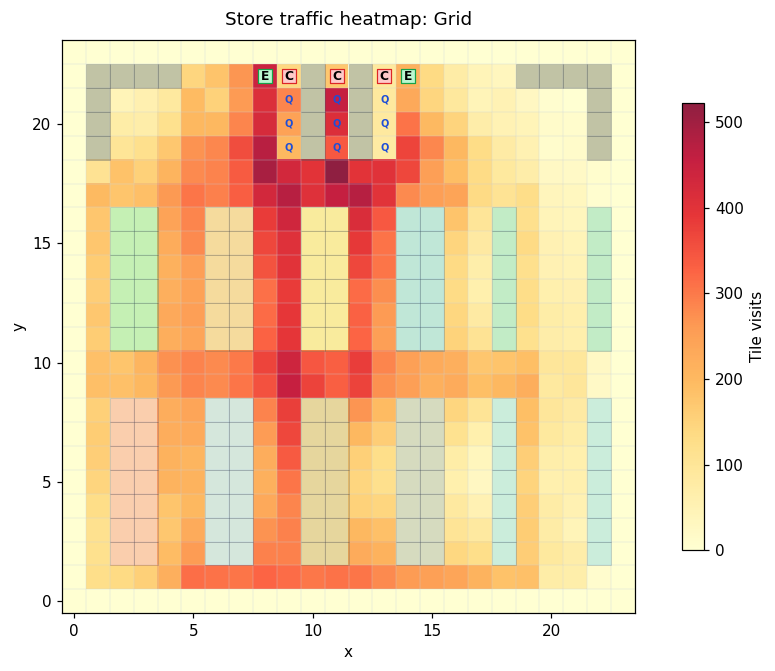
\includegraphics[width=\columnwidth]{heatmap_grid_overall.png}
\caption{Store traffic heatmap for the grid layout. Darker colors indicate higher tile visits across simulation movement paths.}
\Description{Grid-layout store traffic heatmap showing concentrated traffic along central aisles, bottom paths, and checkout-facing corridors.}
\label{fig:grid-traffic-heatmap}
\end{figure}

The shopper-type heatmap in Figure~\ref{fig:grid-shopper-heatmap} shows that mission-driven, loyal, bargain-hunter, and impulse-buyer agents still use the central route structure, while browser agents concentrate more heavily near upper browsing and checkout-adjacent areas. This supports the completion-time results: grid is efficient because it channels movement into direct paths, but it provides less broad product-zone exposure than the loop layout. The pattern is consistent with layout-optimization studies that connect in-store movement structure with operational performance \citep{hwangbo2017,pantano2021}.

\begin{figure}[t]
\centering
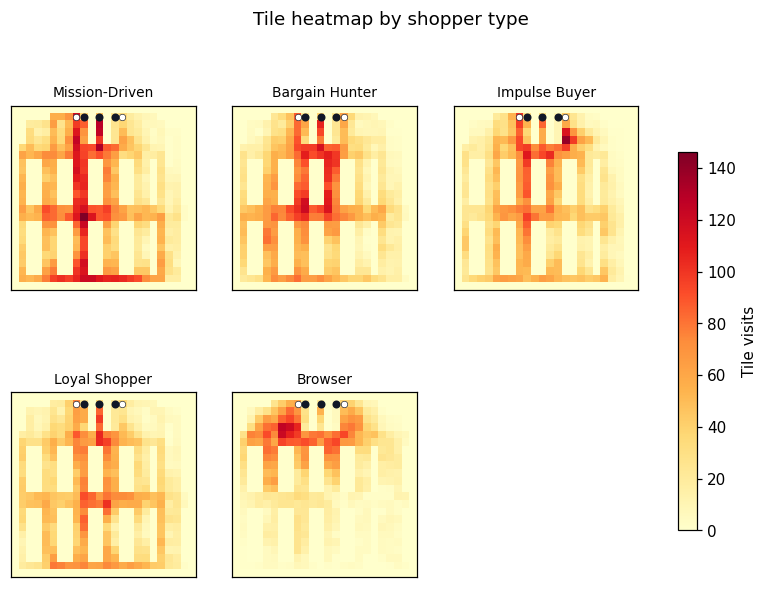
\includegraphics[width=\columnwidth]{heatmap_grid_shoppers.png}
\caption{Grid layout tile heatmaps by shopper type. The panels show how different shopper profiles distribute their movement within the same grid environment.}
\Description{Grid-layout shopper-type heatmaps for mission-driven, bargain-hunter, impulse-buyer, loyal-shopper, and browser agents.}
\label{fig:grid-shopper-heatmap}
\end{figure}

\subsection{Loop Layout Traffic Heatmaps}

The loop heatmaps show the clearest guided-circulation pattern. Figure~\ref{fig:loop-traffic-heatmap} concentrates visits along the perimeter route, with heavy traffic on the left, bottom, and right circulation paths. This supports the interpretation that loop layout increases exposure by pulling shoppers through a repeated route around the store rather than allowing them to move only through the shortest path to planned items.

\begin{figure}[t]
\centering
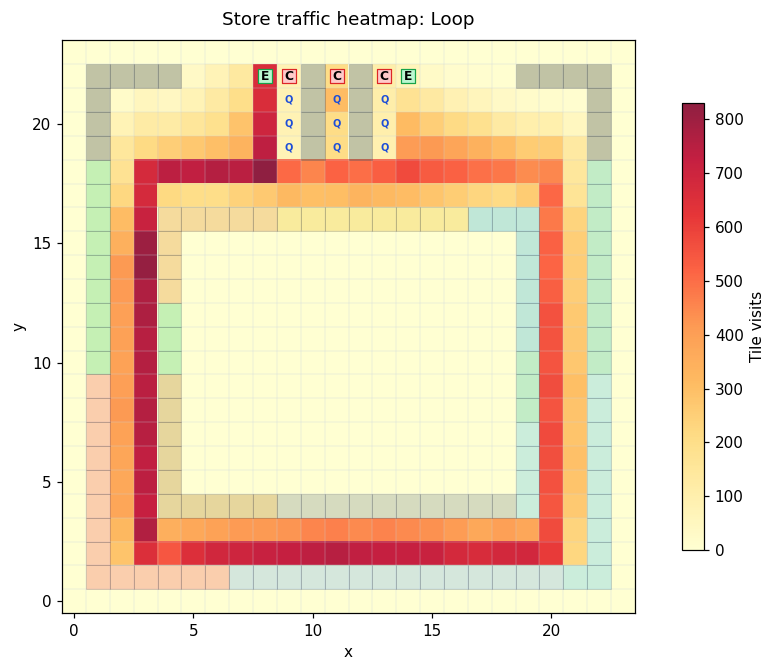
\includegraphics[width=\columnwidth]{heatmap_loop_overall.png}
\caption{Store traffic heatmap for the loop layout. Darker colors indicate stronger use of the racetrack-style circulation path.}
\Description{Loop-layout store traffic heatmap showing strong perimeter movement around the store.}
\label{fig:loop-traffic-heatmap}
\end{figure}

Figure~\ref{fig:loop-shopper-heatmap} shows that the loop path appears across all shopper types, although the intensity differs. Mission-driven and loyal shoppers still follow the guided route, while browsers use a less complete version of the same circulation structure. This explains why loop performs well for planned-list completion and unplanned purchases: the path improves product-zone coverage and repeated exposure. The same structure can also increase trip time and crowding, which is why the loop layout is not always the fastest layout. This interpretation is consistent with studies linking in-store travel distance and product exposure to unplanned spending \citep{hui2013,bellini2017,kacen2012}.

\begin{figure}[t]
\centering
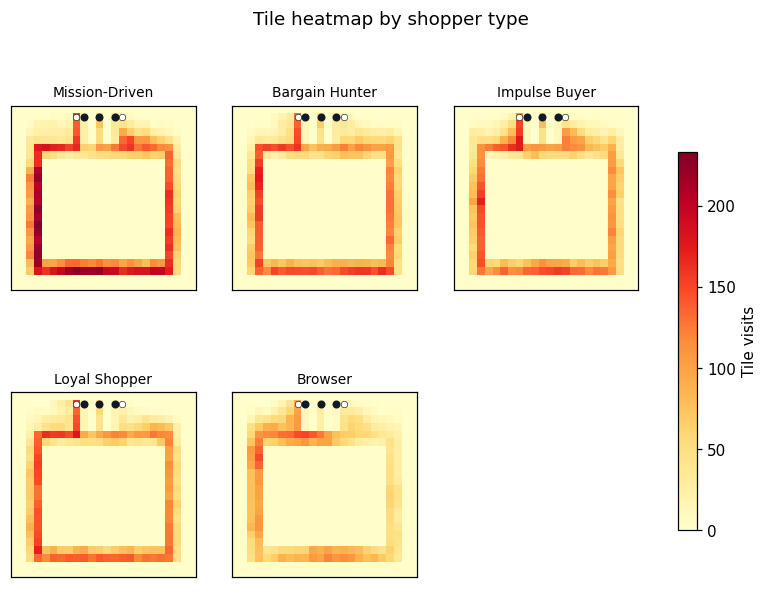
\includegraphics[width=\columnwidth]{heatmap_loop_shoppers.png}
\caption{Loop layout tile heatmaps by shopper type. The panels show how each shopper profile uses the guided racetrack route.}
\Description{Loop-layout shopper-type heatmaps for mission-driven, bargain-hunter, impulse-buyer, loyal-shopper, and browser agents.}
\label{fig:loop-shopper-heatmap}
\end{figure}

\subsection{Free-Flow Layout Traffic Heatmaps}

The free-flow heatmaps show a less regular movement pattern than grid or loop. In Figure~\ref{fig:freeflow-traffic-heatmap}, traffic is strongest near the upper store region and selected internal product islands, but the lower and outer areas receive less systematic coverage. This supports the result that free-flow can encourage exploration while still producing weaker planned-list completion and more items not found.

\begin{figure}[t]
\centering
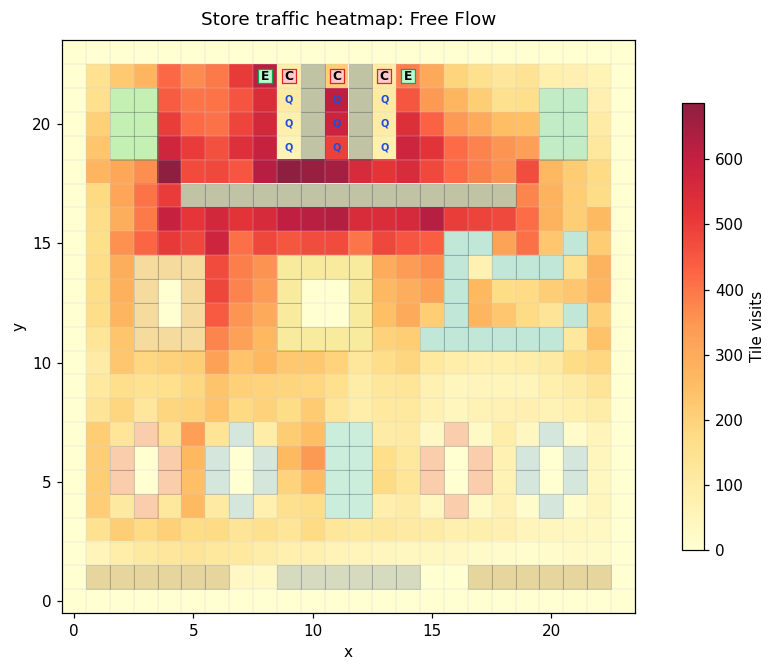
\includegraphics[width=\columnwidth]{heatmap_freeflow_overall.png}
\caption{Store traffic heatmap for the free-flow layout. Darker colors indicate high-traffic areas created by open circulation and product islands.}
\Description{Free-flow store traffic heatmap showing high visits near upper product areas and less systematic lower-store coverage.}
\label{fig:freeflow-traffic-heatmap}
\end{figure}

The shopper-type panels in Figure~\ref{fig:freeflow-shopper-heatmap} show that different profiles do not converge on one dominant route in the same way they do in the loop layout. Browsers concentrate strongly around selected browsing zones, while list-carrying shoppers show lighter and more fragmented coverage. This explains why free-flow generated some unplanned purchases but underperformed in search reliability: the layout offers freedom, but it does not guarantee systematic category exposure. The pattern is consistent with grocery product-arrangement research showing that shoppers rely on expected category relationships when searching for items \citep{seva2019,andrada2020}.

\begin{figure}[t]
\centering
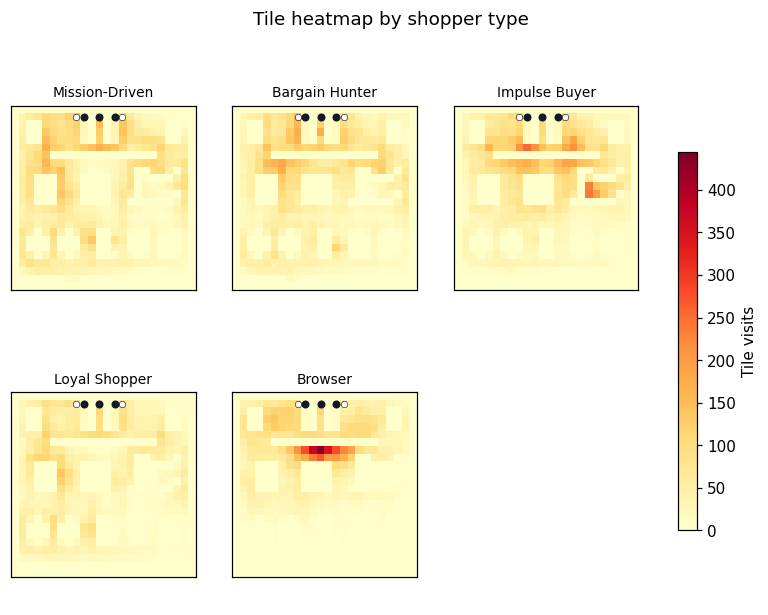
\includegraphics[width=\columnwidth]{heatmap_freeflow_shoppers.png}
\caption{Free-flow layout tile heatmaps by shopper type. The panels show more fragmented movement across shopper profiles compared with the grid and loop layouts.}
\Description{Free-flow shopper-type heatmaps for mission-driven, bargain-hunter, impulse-buyer, loyal-shopper, and browser agents.}
\label{fig:freeflow-shopper-heatmap}
\end{figure}

\subsection{Average Completion Time}

Average completion time measures shopping efficiency. At the highest density, the grid layout was fastest in five of the six shopper mixes: equal, bargain-hunter, impulse-buyer, loyal-shopper, and browser. For example, impulse-buyer trips averaged 202.8 minutes in grid, 238.7 minutes in loop, and 277.0 minutes in free-flow. Browser trips showed the largest search-time gap: 245.2 minutes in grid, 306.3 in loop, and 325.9 in free-flow. The mission-driven mix was the one exception, where loop was slightly fastest at 201.0 minutes, followed by grid at 202.8 and free-flow at 213.2.

\begin{figure}[t]
\centering
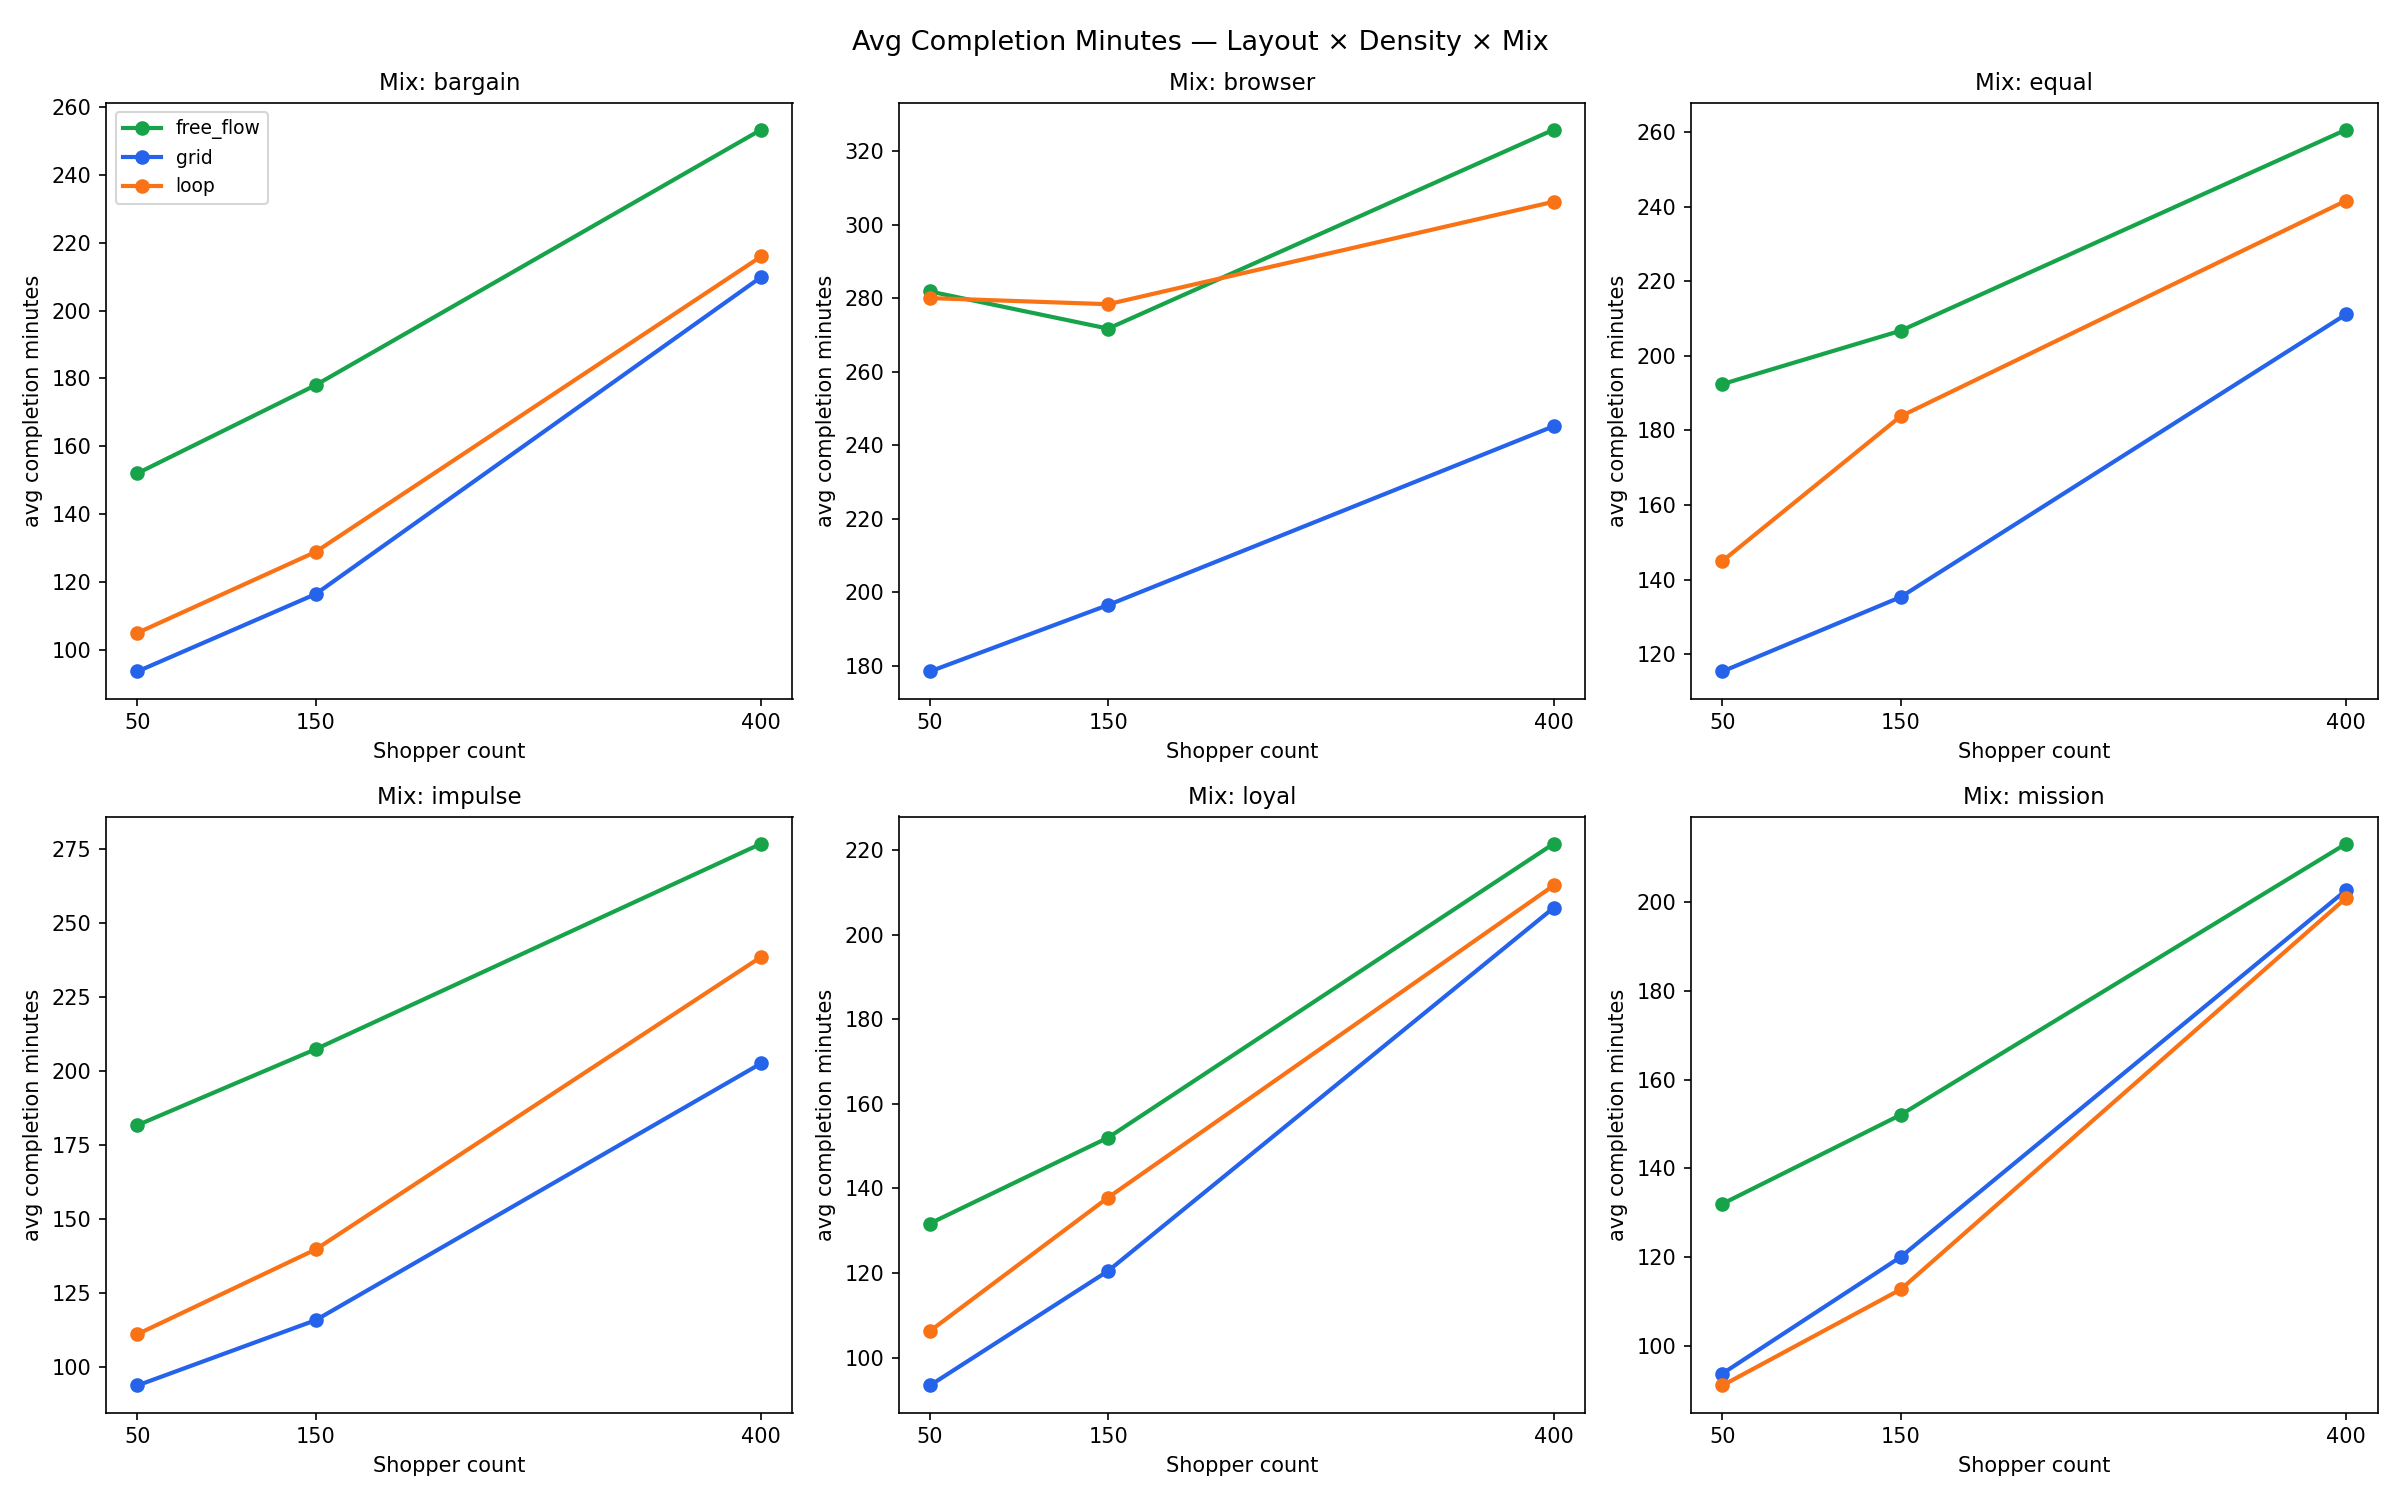
\includegraphics[width=\columnwidth]{linechart_avg_completion_minutes.png}
\vspace{0.12in}
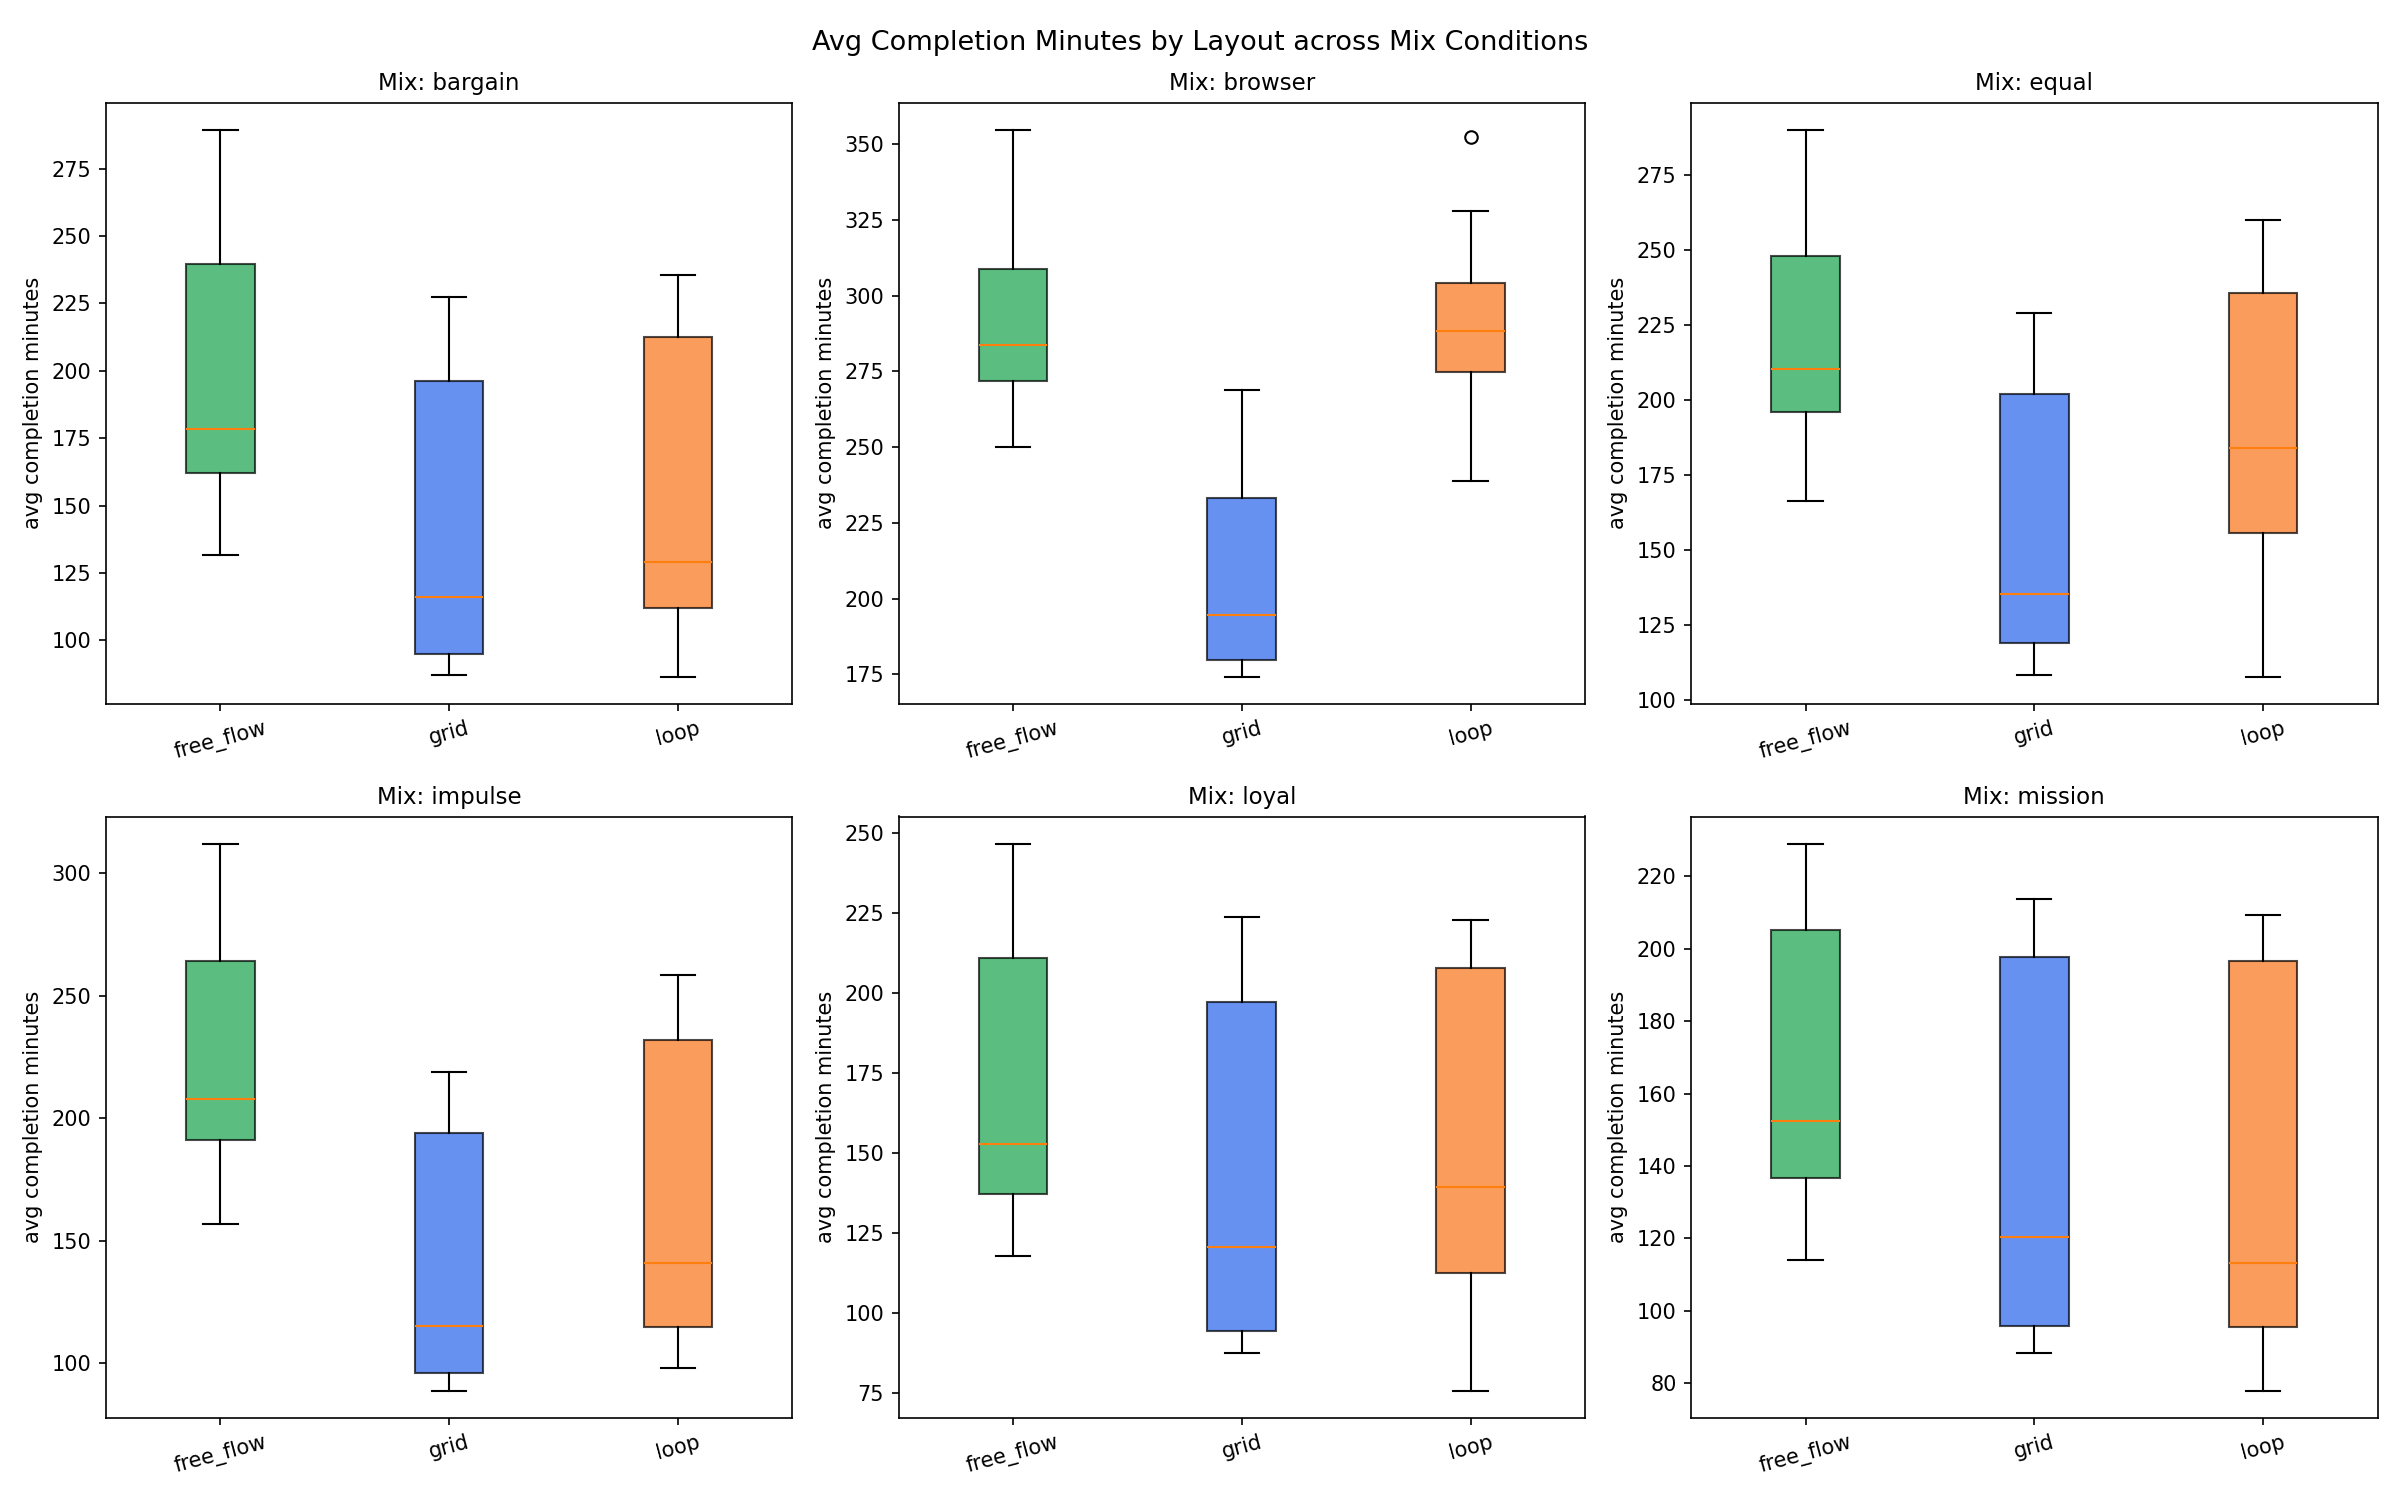
\includegraphics[width=0.82\columnwidth]{boxplot_avg_completion_minutes.png}
\caption{Average completion minutes by density, layout, and shopper mix. The line chart shows how completion time changes as density increases, while the boxplot summarizes the distribution of run-level completion times.}
\Description{Average completion minutes line chart and boxplot for grid, loop, and free-flow layouts across shopper mixes.}
\label{fig:completion-time}
\end{figure}

Figure~\ref{fig:completion-time} shows that completion time increases as density rises, but the grid layout keeps trip duration lower for most shopper populations. This supports the interpretation that structured aisles reduce movement uncertainty and keep routes more predictable under crowd pressure. Free-flow produces the slowest and most variable completion times because exploratory movement and irregular shelf placement increase search costs. The finding aligns with retail-layout and indoor-positioning research showing that movement data can guide layout optimization \citep{hwangbo2017,ozgormus2020}, and with agent-based store-density work showing that density changes layout performance \citep{pantano2021}.

\subsection{Planned-List Completion}

Planned-list completion measures how much of a shopper's intended list was successfully purchased. This outcome applies to the equal, mission-driven, bargain-hunter, impulse-buyer, and loyal-shopper mixes. Browsers have no planned list, so planned-completion values for the browser condition are not behaviorally meaningful.

At 400 shoppers, loop produced the strongest planned-list completion in all five list-carrying mixes. Planned completion was 0.886 for equal, 0.894 for mission-driven, 0.901 for bargain-hunter, 0.889 for impulse-buyer, and 0.938 for loyal-shopper mixes. This result shows that speed and complete list fulfillment are different outcomes: grid is usually faster, but loop gives shoppers more systematic exposure to product zones before checkout.

\begin{figure}[t]
\centering
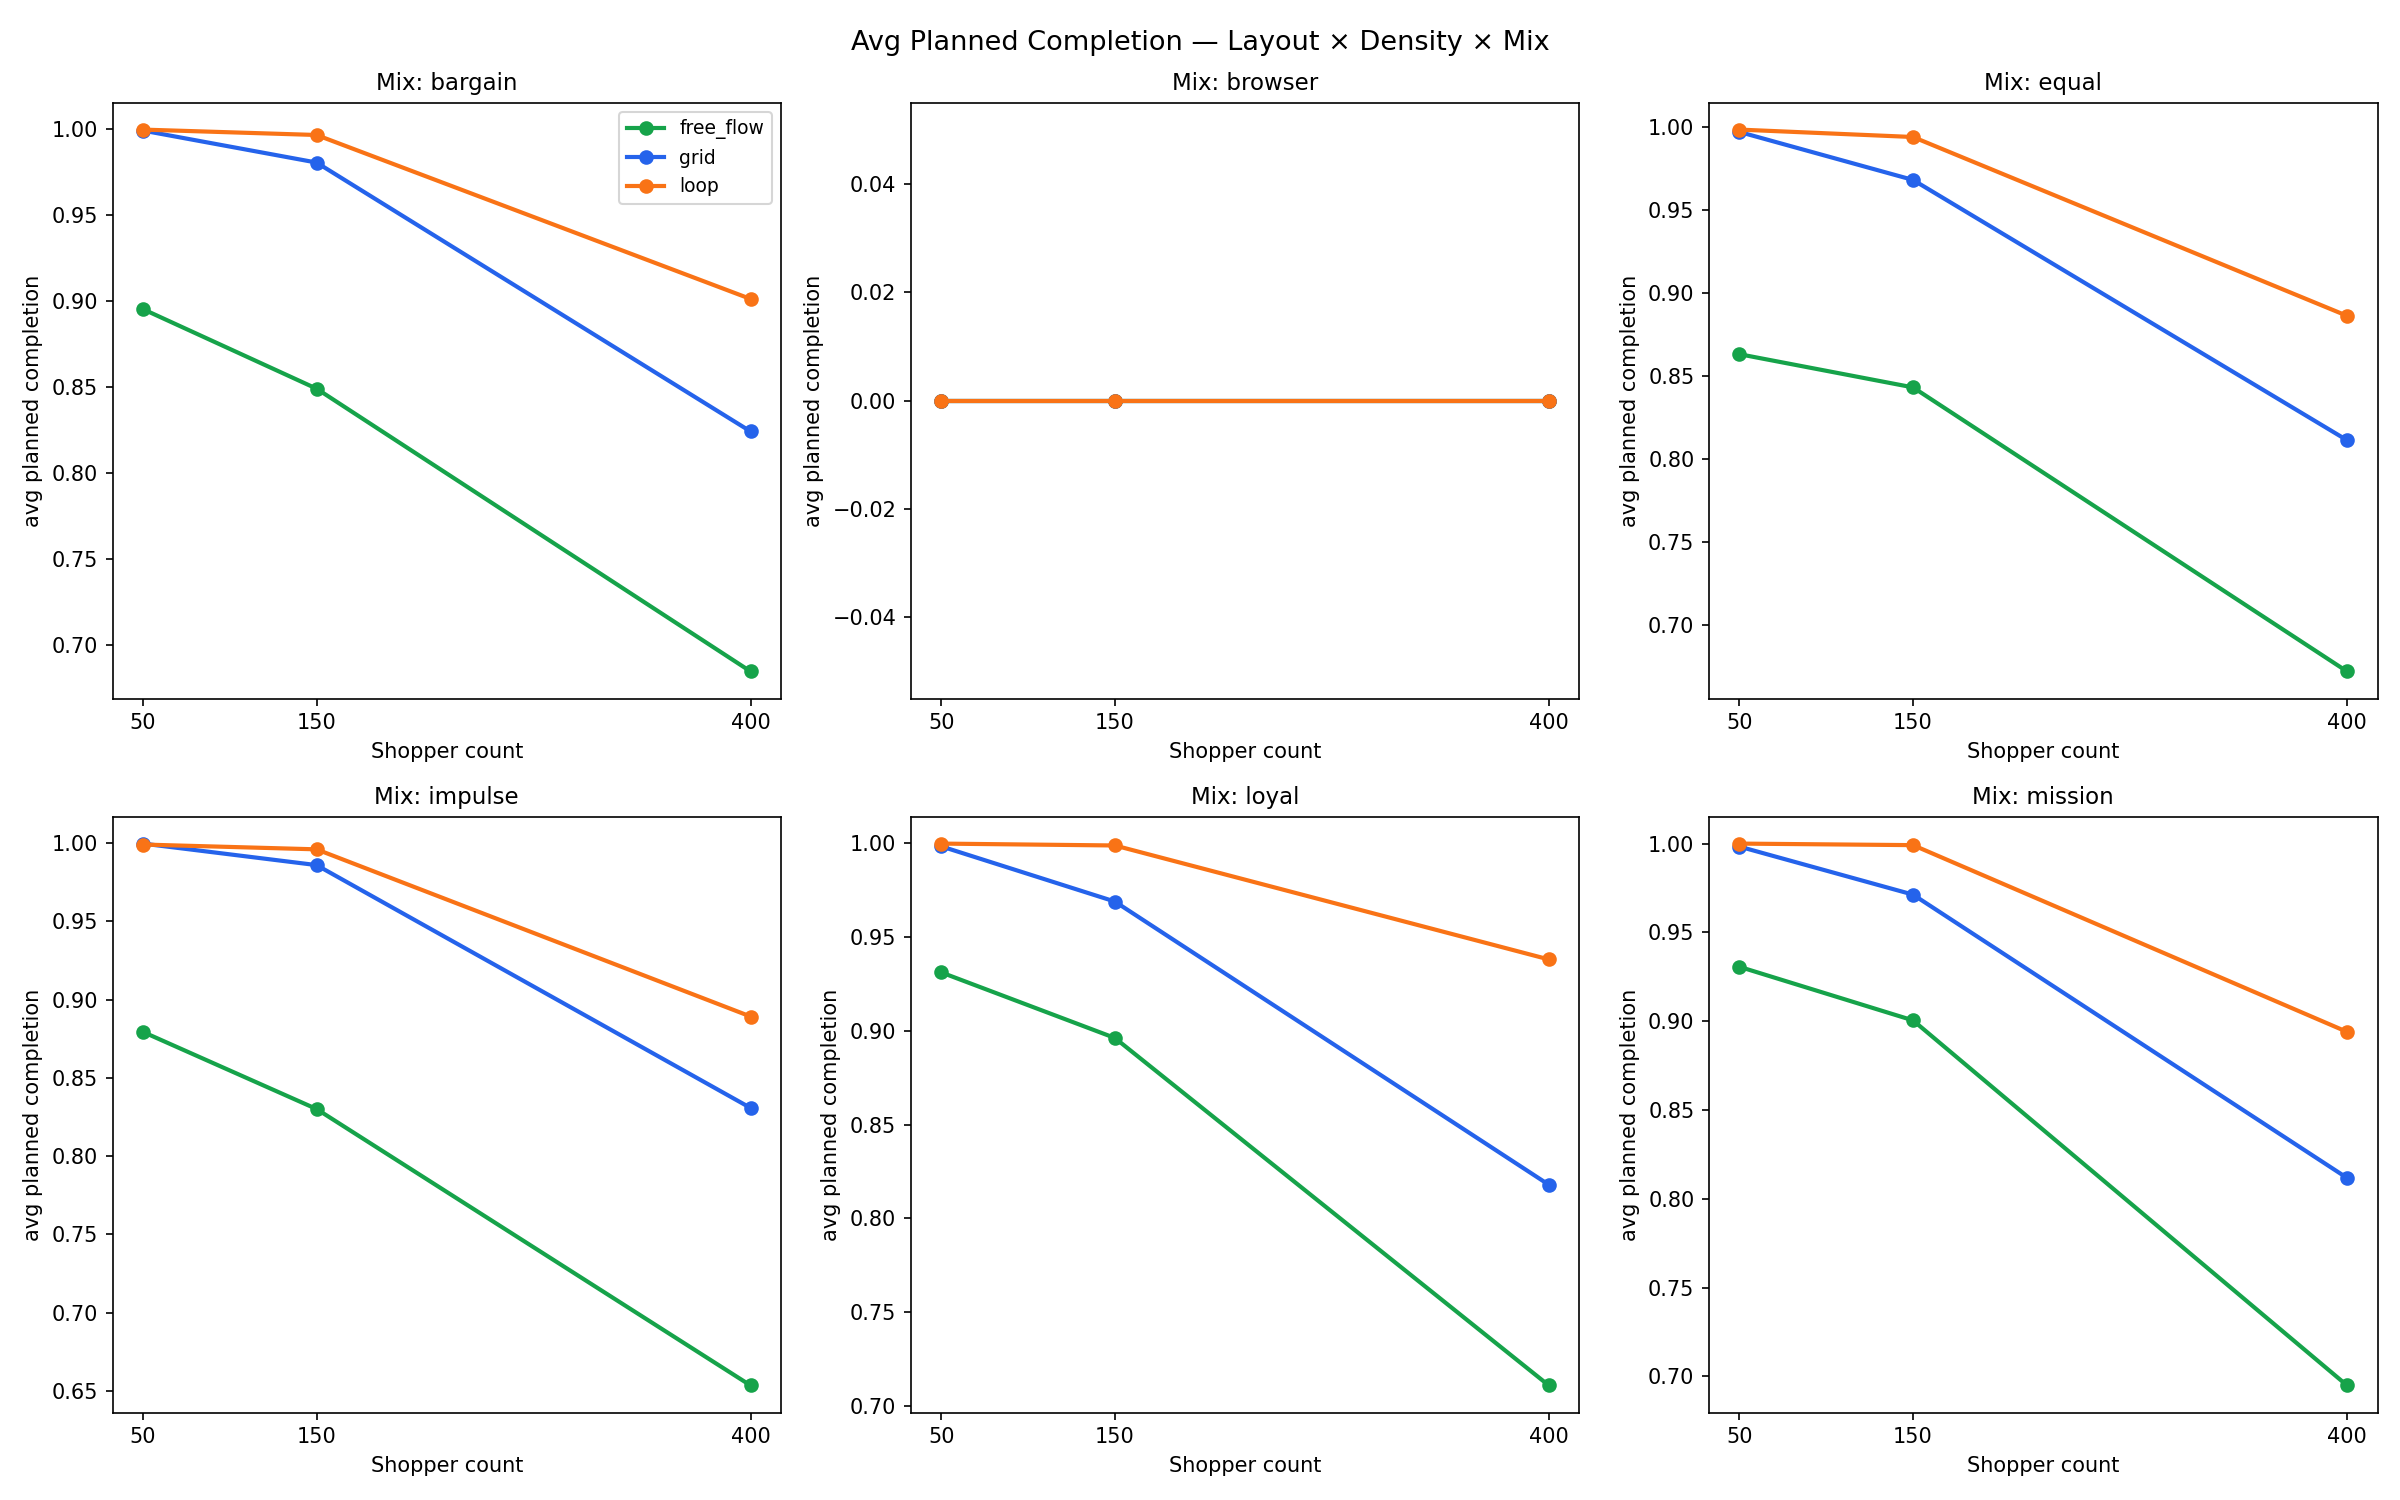
\includegraphics[width=\columnwidth]{linechart_avg_planned_completion.png}
\vspace{0.12in}
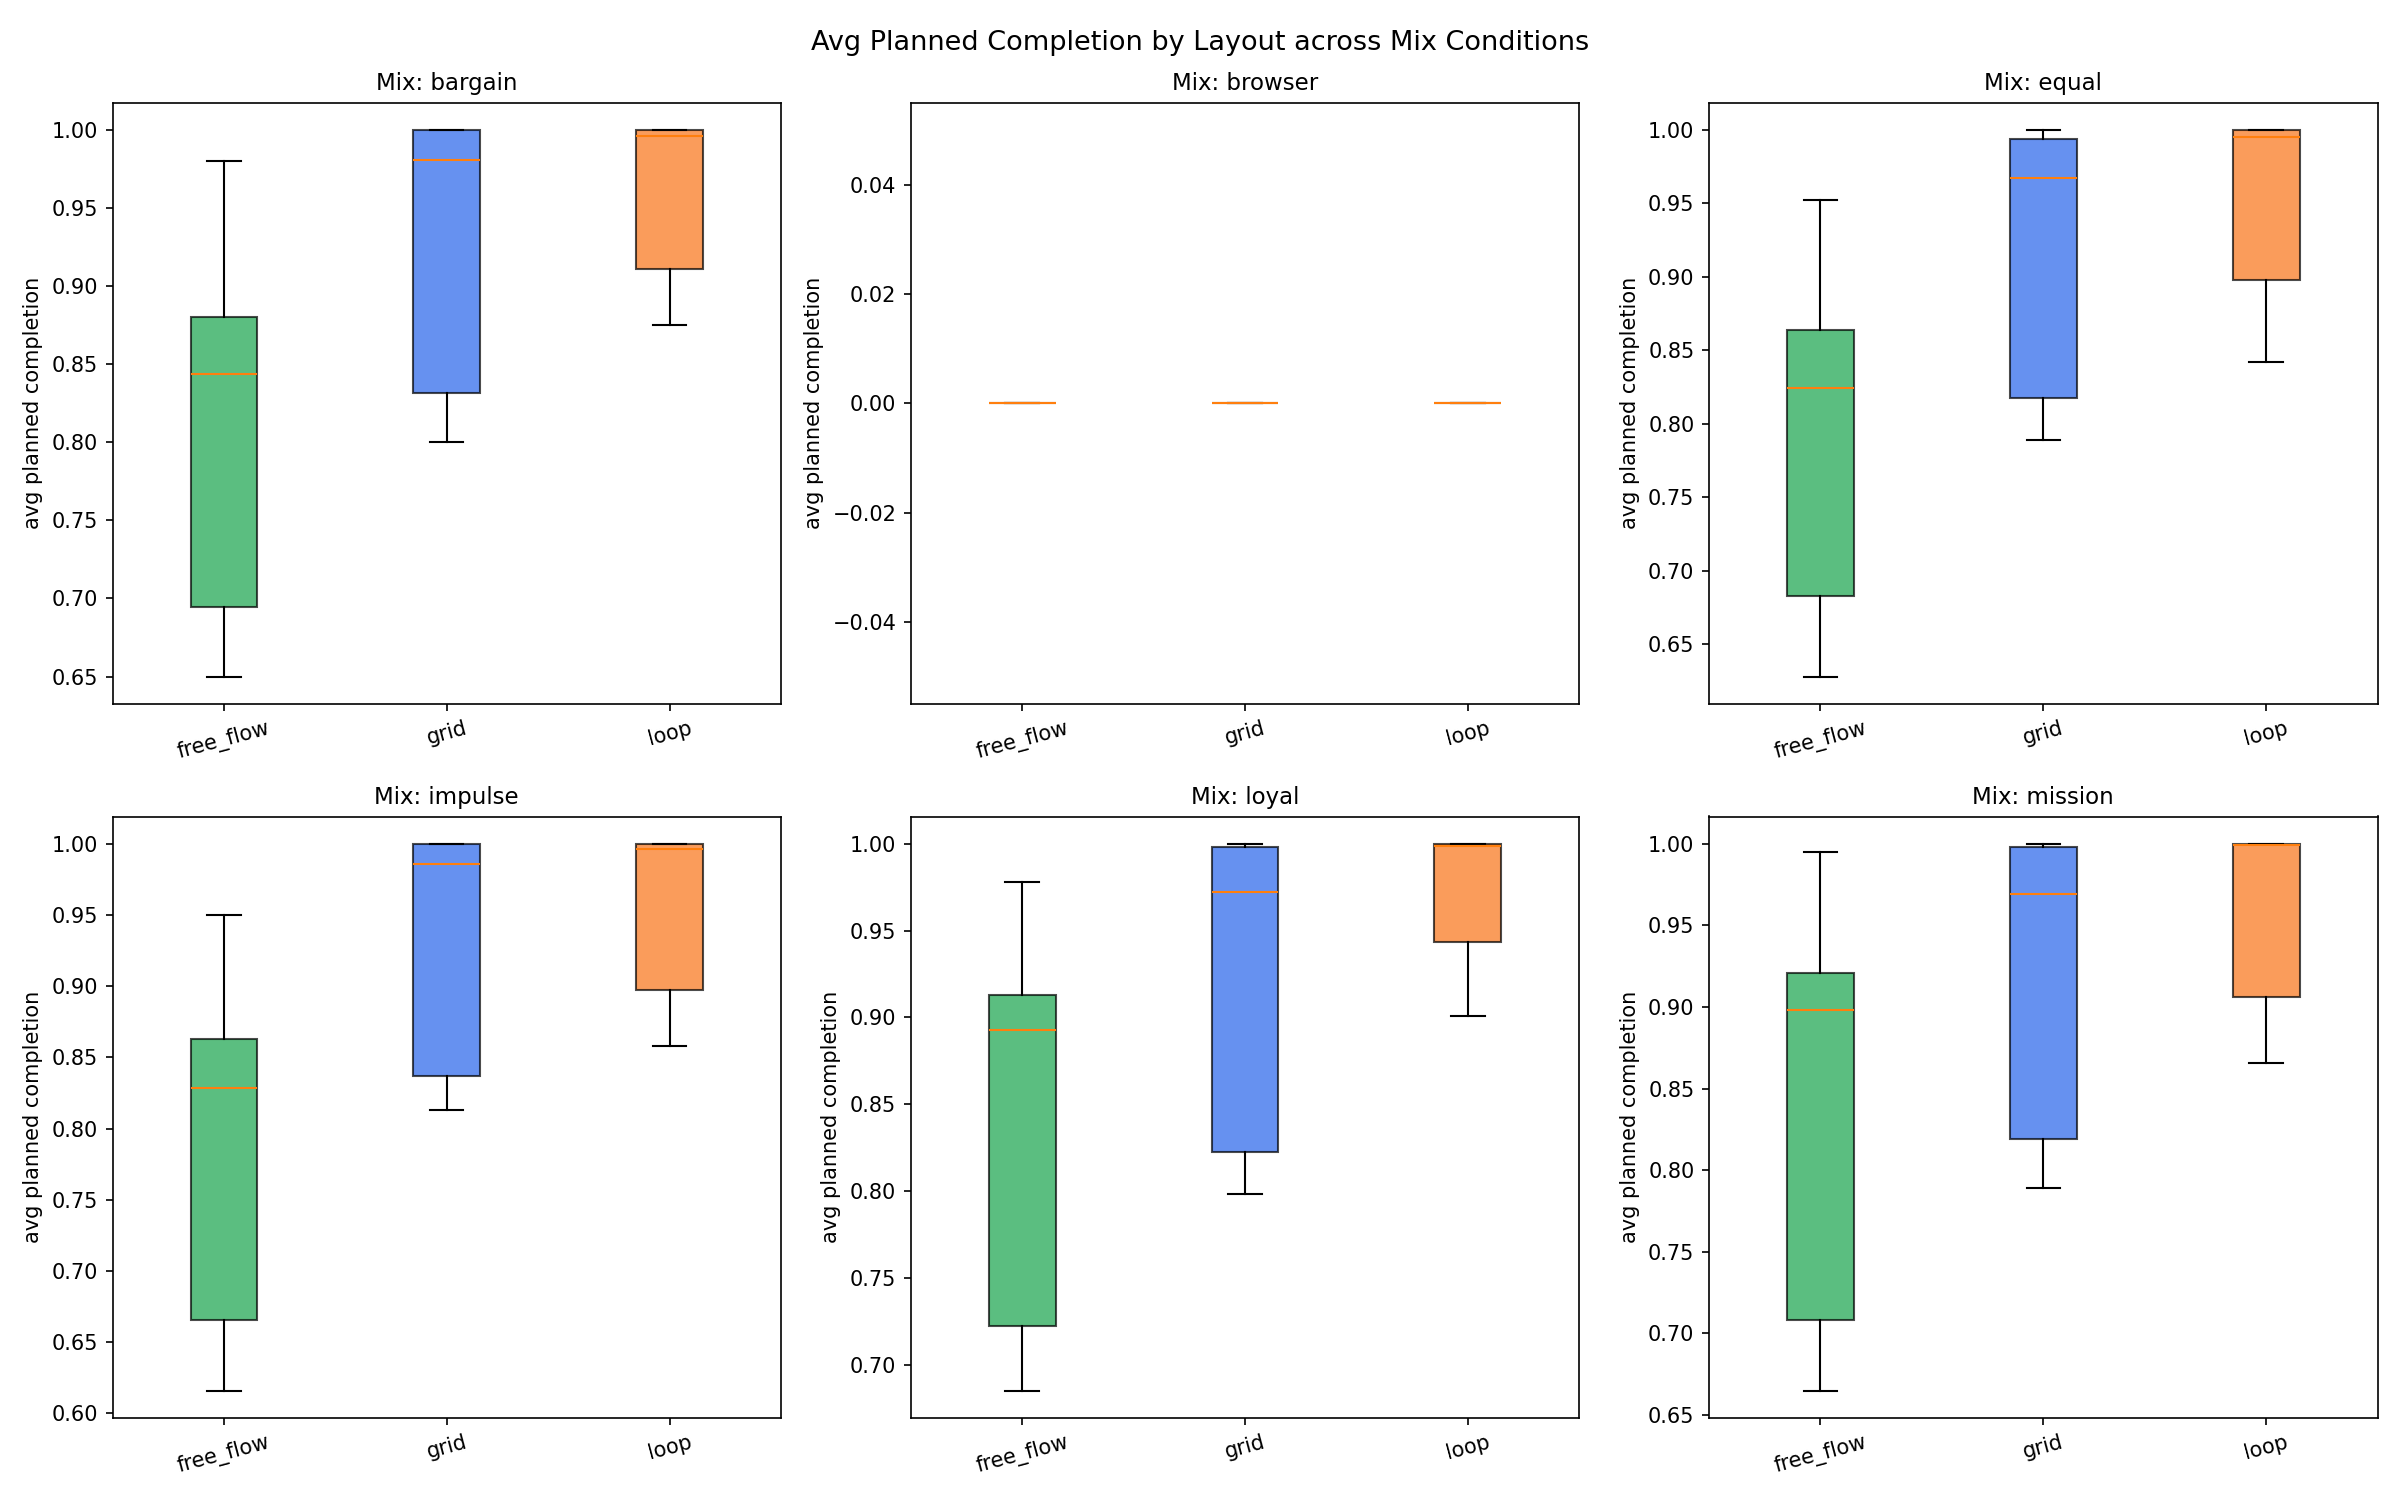
\includegraphics[width=0.82\columnwidth]{boxplot_avg_planned_completion.png}
\caption{Planned-list completion by density, layout, and shopper mix. The line chart shows list-completion trends across density, while the boxplot summarizes run-level planned-completion distributions.}
\Description{Planned-list completion line chart and boxplot for grid, loop, and free-flow layouts across shopper mixes.}
\label{fig:planned-completion}
\end{figure}

Figure~\ref{fig:planned-completion} shows that loop performs best for planned-list fulfillment among list-carrying shoppers, especially at high density. The guided route gives shoppers repeated opportunities to pass category zones, which helps them complete more of their lists even when trip times are not the shortest. This interpretation is consistent with product-arrangement research showing that grocery search depends on expected relationships among categories \citep{seva2019}, and with Philippine grocery-layout research identifying shelf organization, aisle space, and product availability as important layout variables \citep{andrada2020}.

\subsection{Items Not Found}

Items not found is the inverse search-failure measure behind planned-list completion. At 400 shoppers, loop produced the fewest missed items among list-carrying mixes: 260.7 for equal, 338.8 for mission-driven, 276.7 for bargain-hunter, 266.1 for impulse-buyer, and 198.2 for loyal-shopper mixes. Free-flow was the weakest layout for this metric, with missed items ranging from 763.0 in the equal mix to 976.3 in the mission-driven mix.

\begin{figure}[t]
\centering
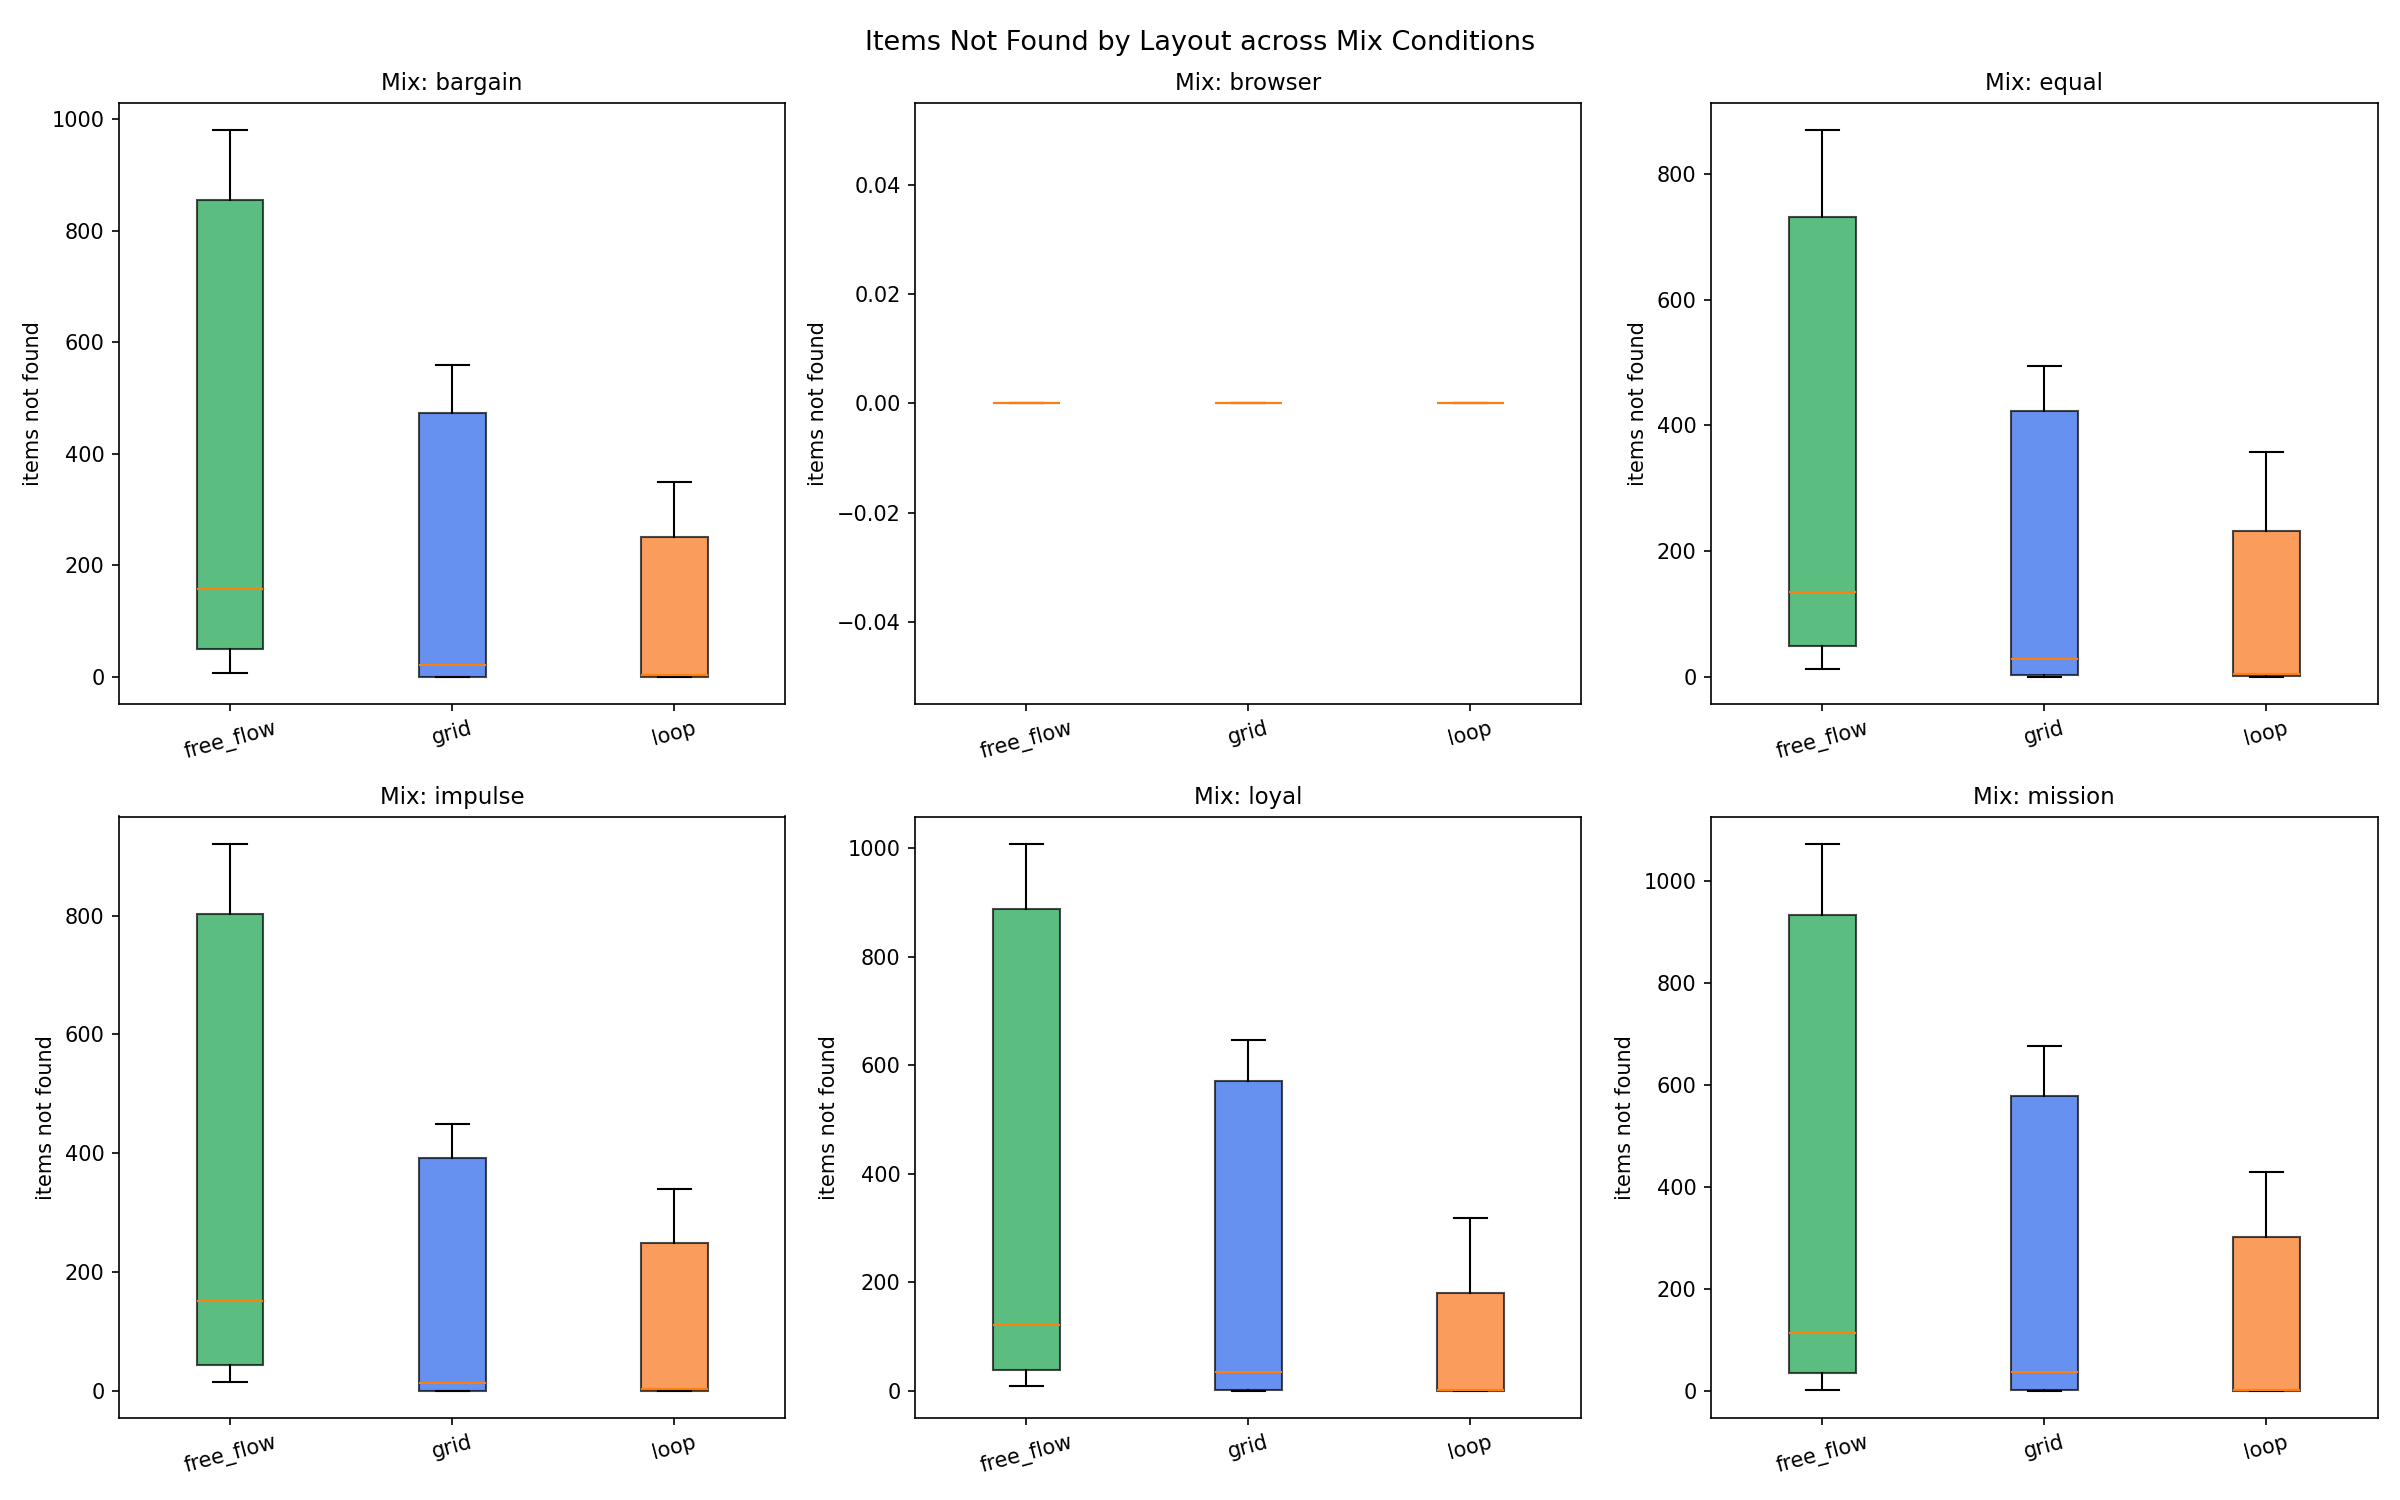
\includegraphics[width=0.90\columnwidth]{boxplot_items_not_found.png}
\caption{Items not found by layout and shopper mix. The boxplot shows how many planned items shoppers failed to locate across simulation runs.}
\Description{Boxplot of items not found for grid, loop, and free-flow layouts across shopper mixes.}
\label{fig:items-not-found}
\end{figure}

Figure~\ref{fig:items-not-found} shows that free-flow creates the highest search-failure burden. This does not mean free-flow prevents movement; rather, it gives shoppers less predictable category coverage. Loop performs better because it carries shoppers through more product zones, reducing the chance that planned items remain unseen. The result supports the importance of category organization and store-layout clarity in grocery shopping \citep{seva2019,andrada2020}.

\subsection{Unplanned Purchases}

Unplanned purchases measure exposure-driven buying beyond the original shopping list. The loop layout generated the most unplanned purchases in every final high-density mix. At 400 shoppers, loop produced 1,725.6 unplanned purchases in the equal mix, 401.6 in the mission-driven mix, 1,430.4 in the bargain-hunter mix, 3,615.0 in the impulse-buyer mix, 725.6 in the loyal-shopper mix, and 2,243.2 in the browser mix.

\begin{figure}[t]
\centering
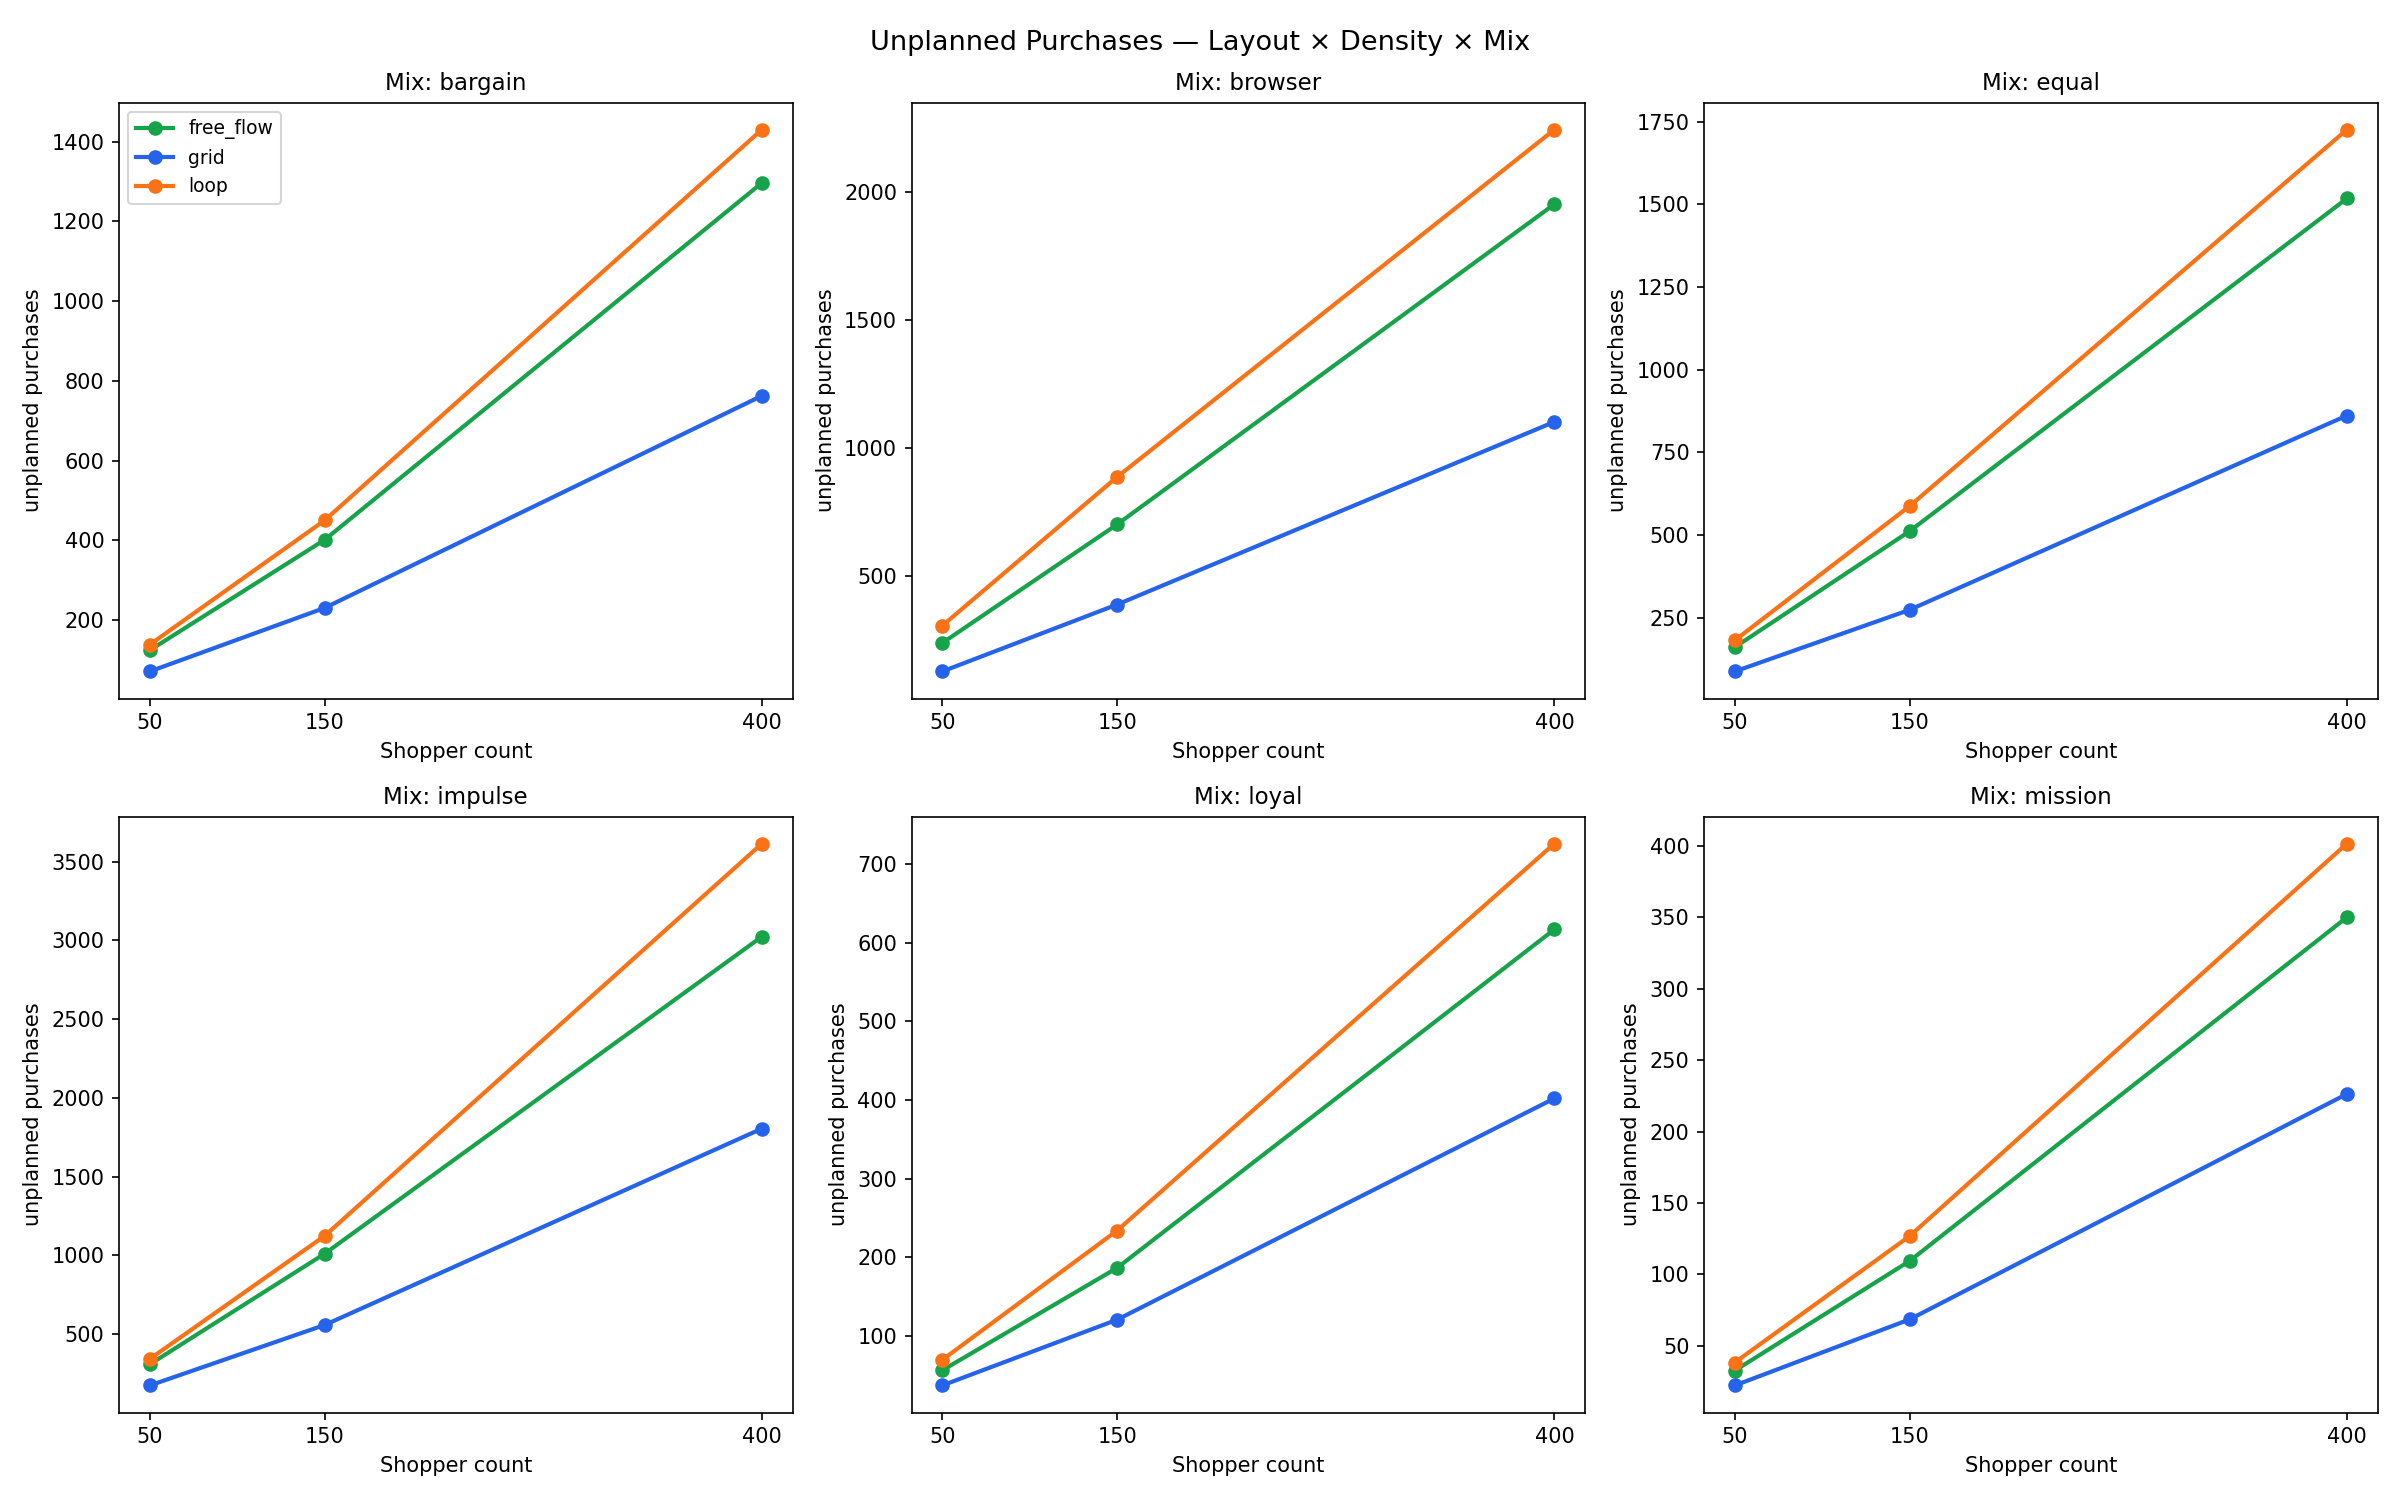
\includegraphics[width=\columnwidth]{linechart_unplanned_purchases.png}
\vspace{0.12in}
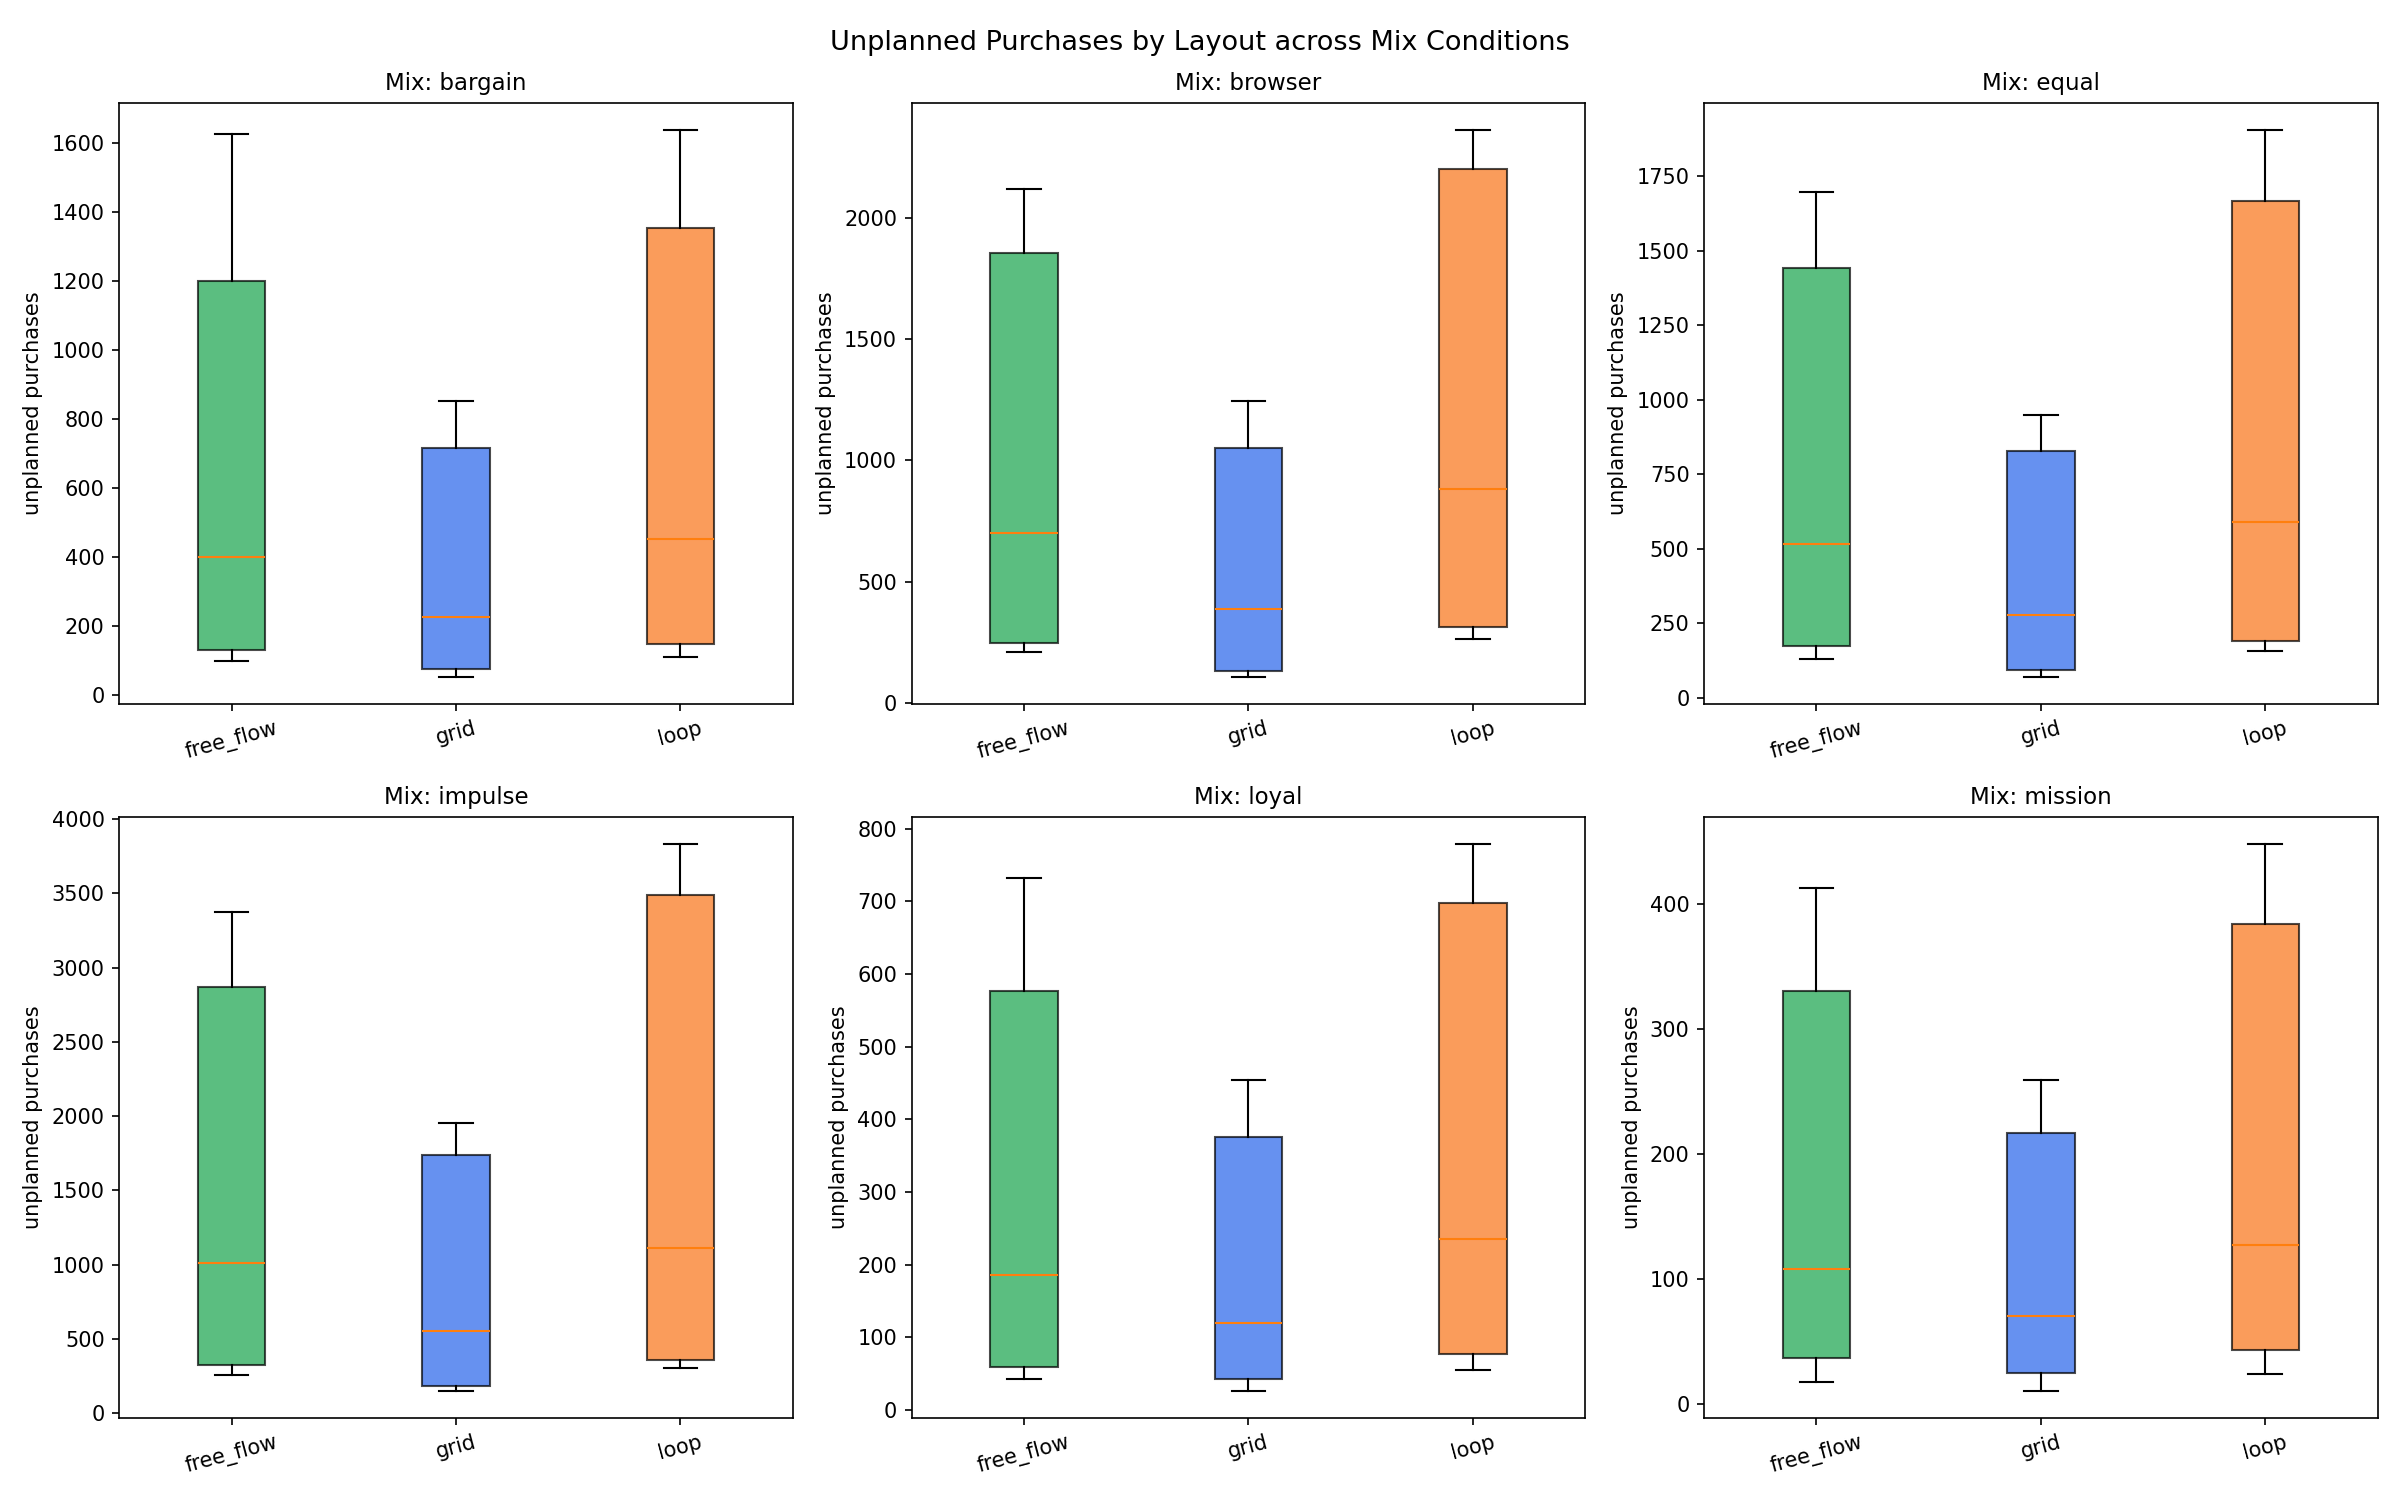
\includegraphics[width=0.82\columnwidth]{boxplot_unplanned_purchases.png}
\caption{Unplanned purchases by density, layout, and shopper mix. The line chart shows how unplanned purchases change as density rises, while the boxplot shows run-level variation.}
\Description{Unplanned-purchase line chart and boxplot for grid, loop, and free-flow layouts across shopper mixes.}
\label{fig:unplanned-purchases}
\end{figure}

Figure~\ref{fig:unplanned-purchases} shows that loop consistently produces the strongest unplanned-purchase pattern. The result supports the exposure mechanism built into the model: a loop path increases repeated product contact, and longer in-store travel has been linked to higher unplanned spending \citep{hui2013}. The pattern also fits impulse-buying research showing that exposure, retail stimuli, promotions, product characteristics, and shopper impulse tendency influence unplanned purchase likelihood \citep{bellini2017,kacen2012,stilley2010}.

\subsection{Completion Rate}

Completion rate measures the proportion of shoppers who successfully finished their trip instead of abandoning. The distribution is generally stable at lower densities, but layout differences become more visible at high density because congestion and queue stress increase. Grid tends to protect completion more effectively in crowd-sensitive mixes because it reduces trip time and lowers the chance that shoppers lose patience before checkout.

\begin{figure}[t]
\centering
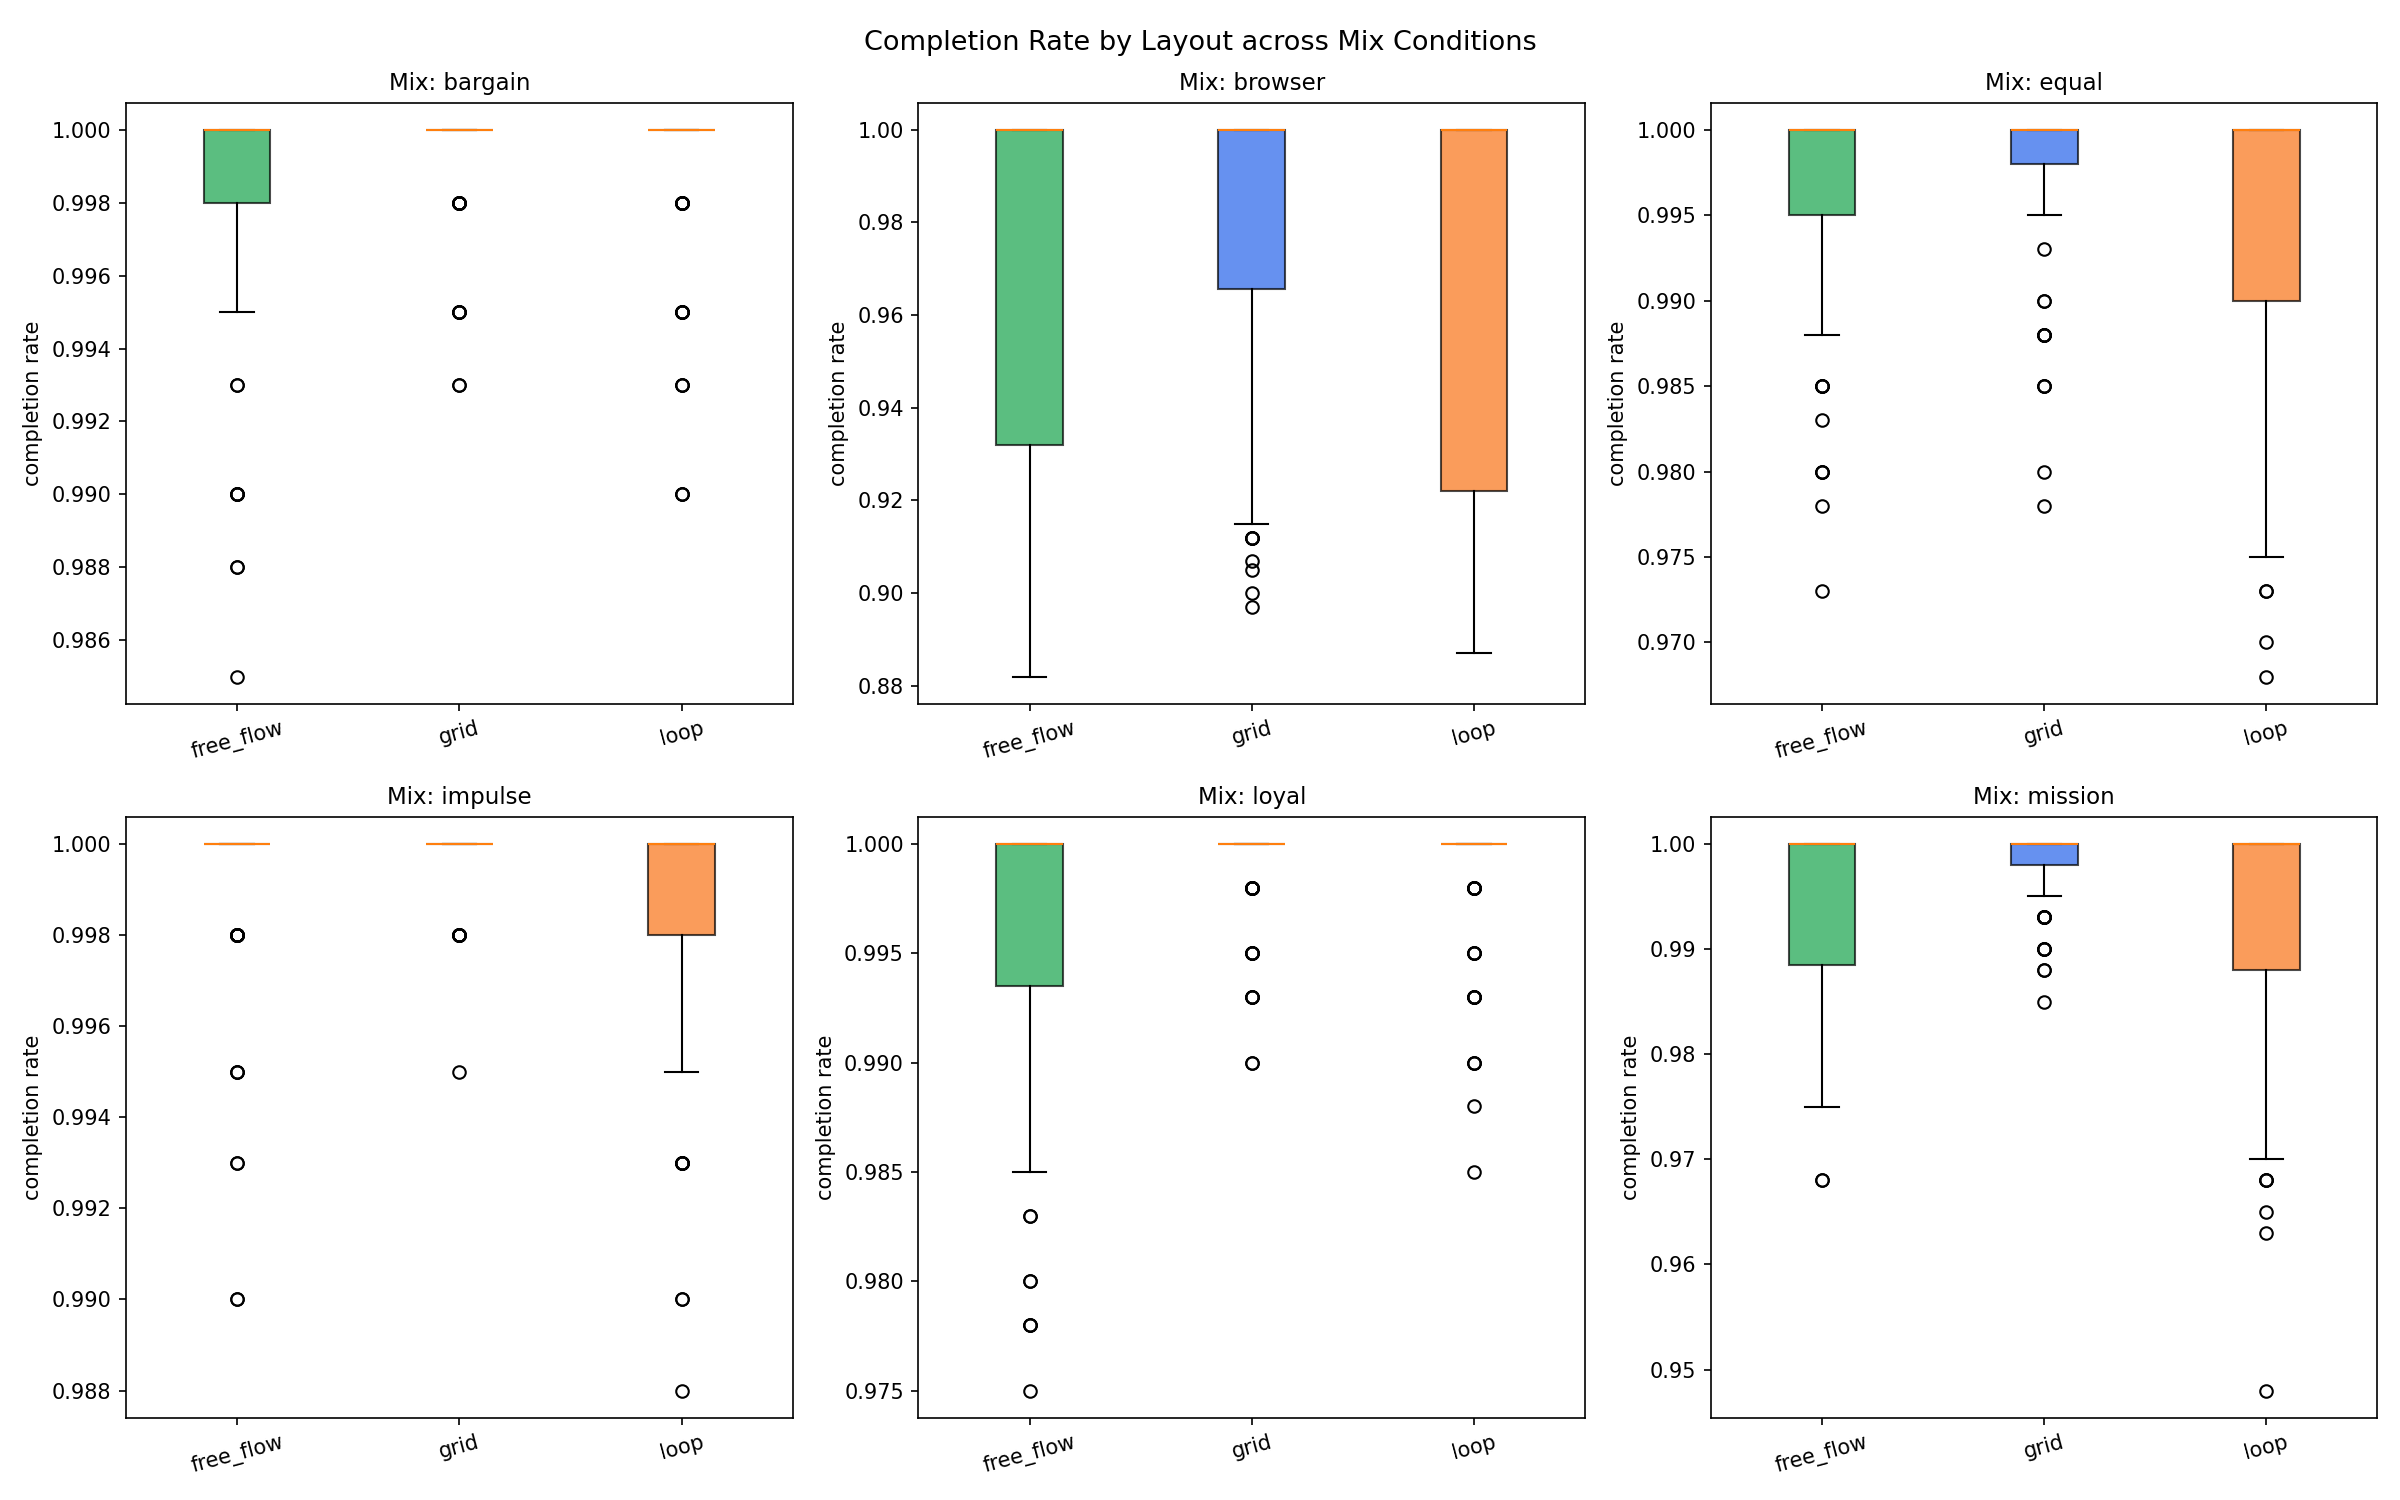
\includegraphics[width=0.90\columnwidth]{boxplot_completion_rate.png}
\caption{Completion rate by layout and shopper mix. The boxplot summarizes run-level completion-rate distributions across the final simulation runs.}
\Description{Boxplot of completion rate for grid, loop, and free-flow layouts across shopper mixes.}
\label{fig:completion-rate}
\end{figure}

Figure~\ref{fig:completion-rate} shows that completion rate is not only a checkout issue; it is also affected by the route and search experience before checkout. Layouts that reduce search time and crowding pressure are more likely to keep shoppers in the store until the trip is completed. This supports the broader interpretation that layout influences operational flow, not only purchasing exposure \citep{hwangbo2017,pantano2021}.

\subsection{Abandonment Rate}

Abandonment rate is the failure outcome corresponding to completion rate. Abandonment was small at lower densities but became important at 400 shoppers. Browser shoppers showed the highest abandonment pressure: 5.8\% in grid, 7.9\% in free-flow, and 8.6\% in loop. In contrast, abandonment was below 0.5\% for impulse and bargain-hunter shoppers at high density.

\begin{figure}[t]
\centering
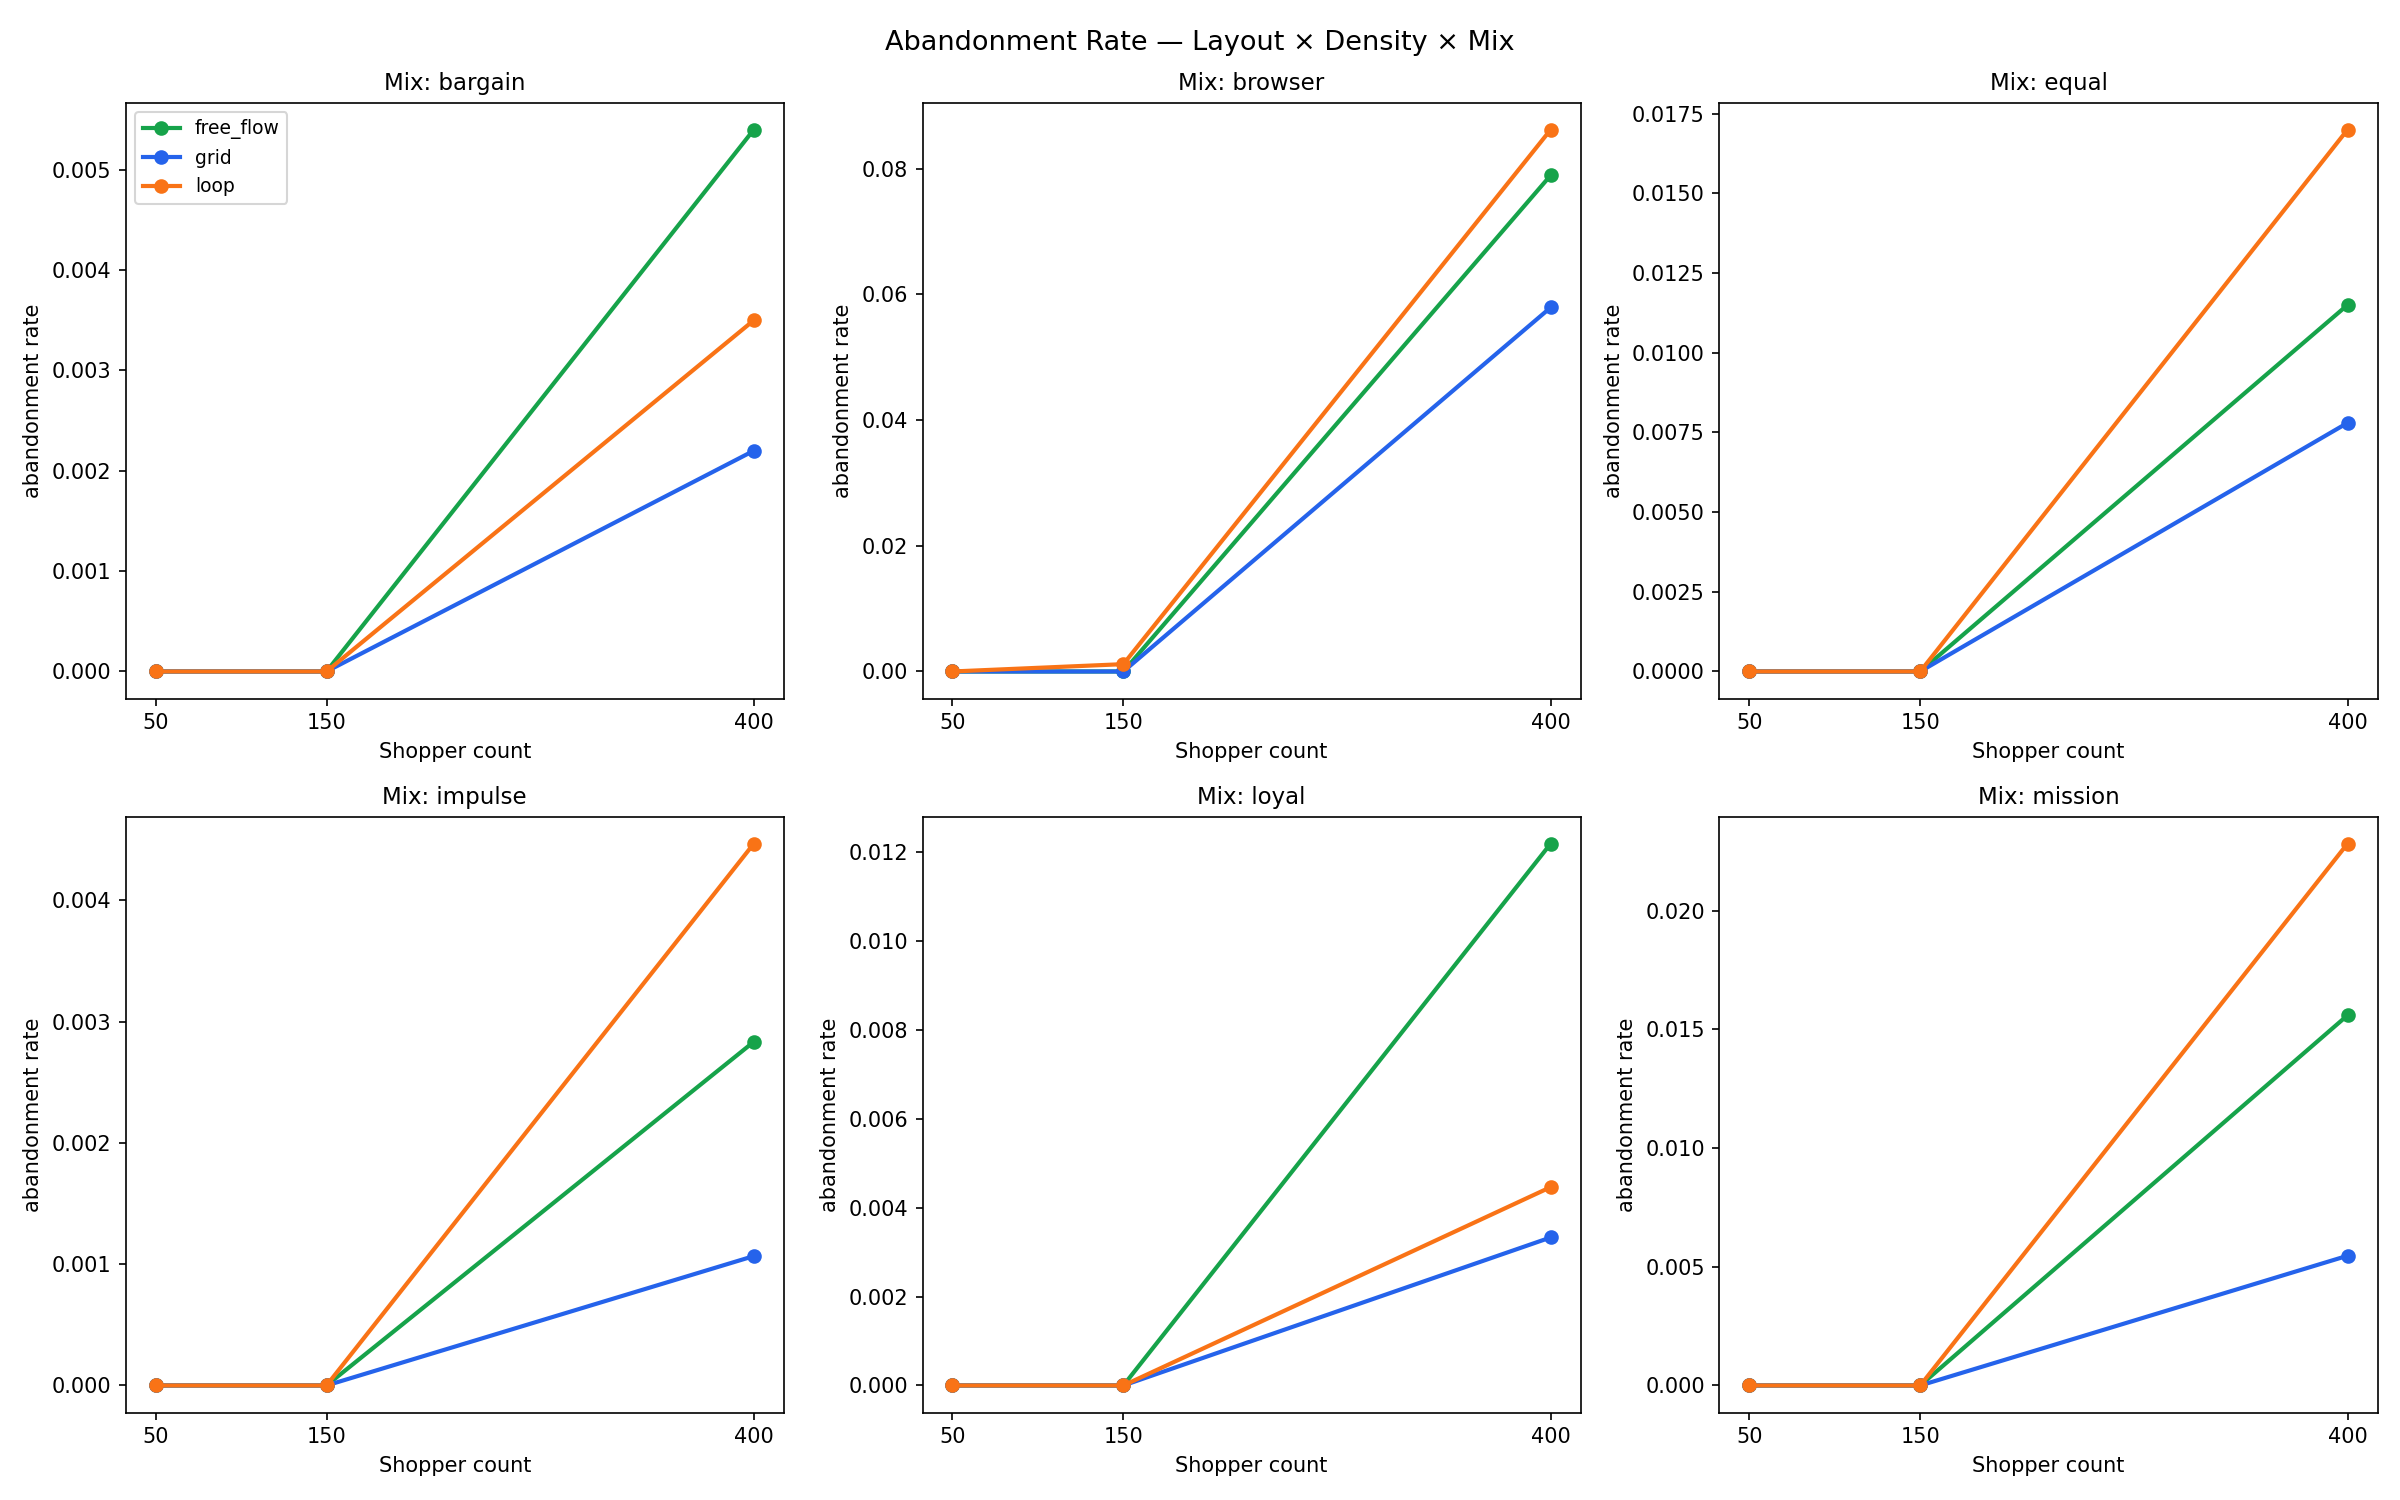
\includegraphics[width=\columnwidth]{linechart_abandonment_rate.png}
\vspace{0.12in}
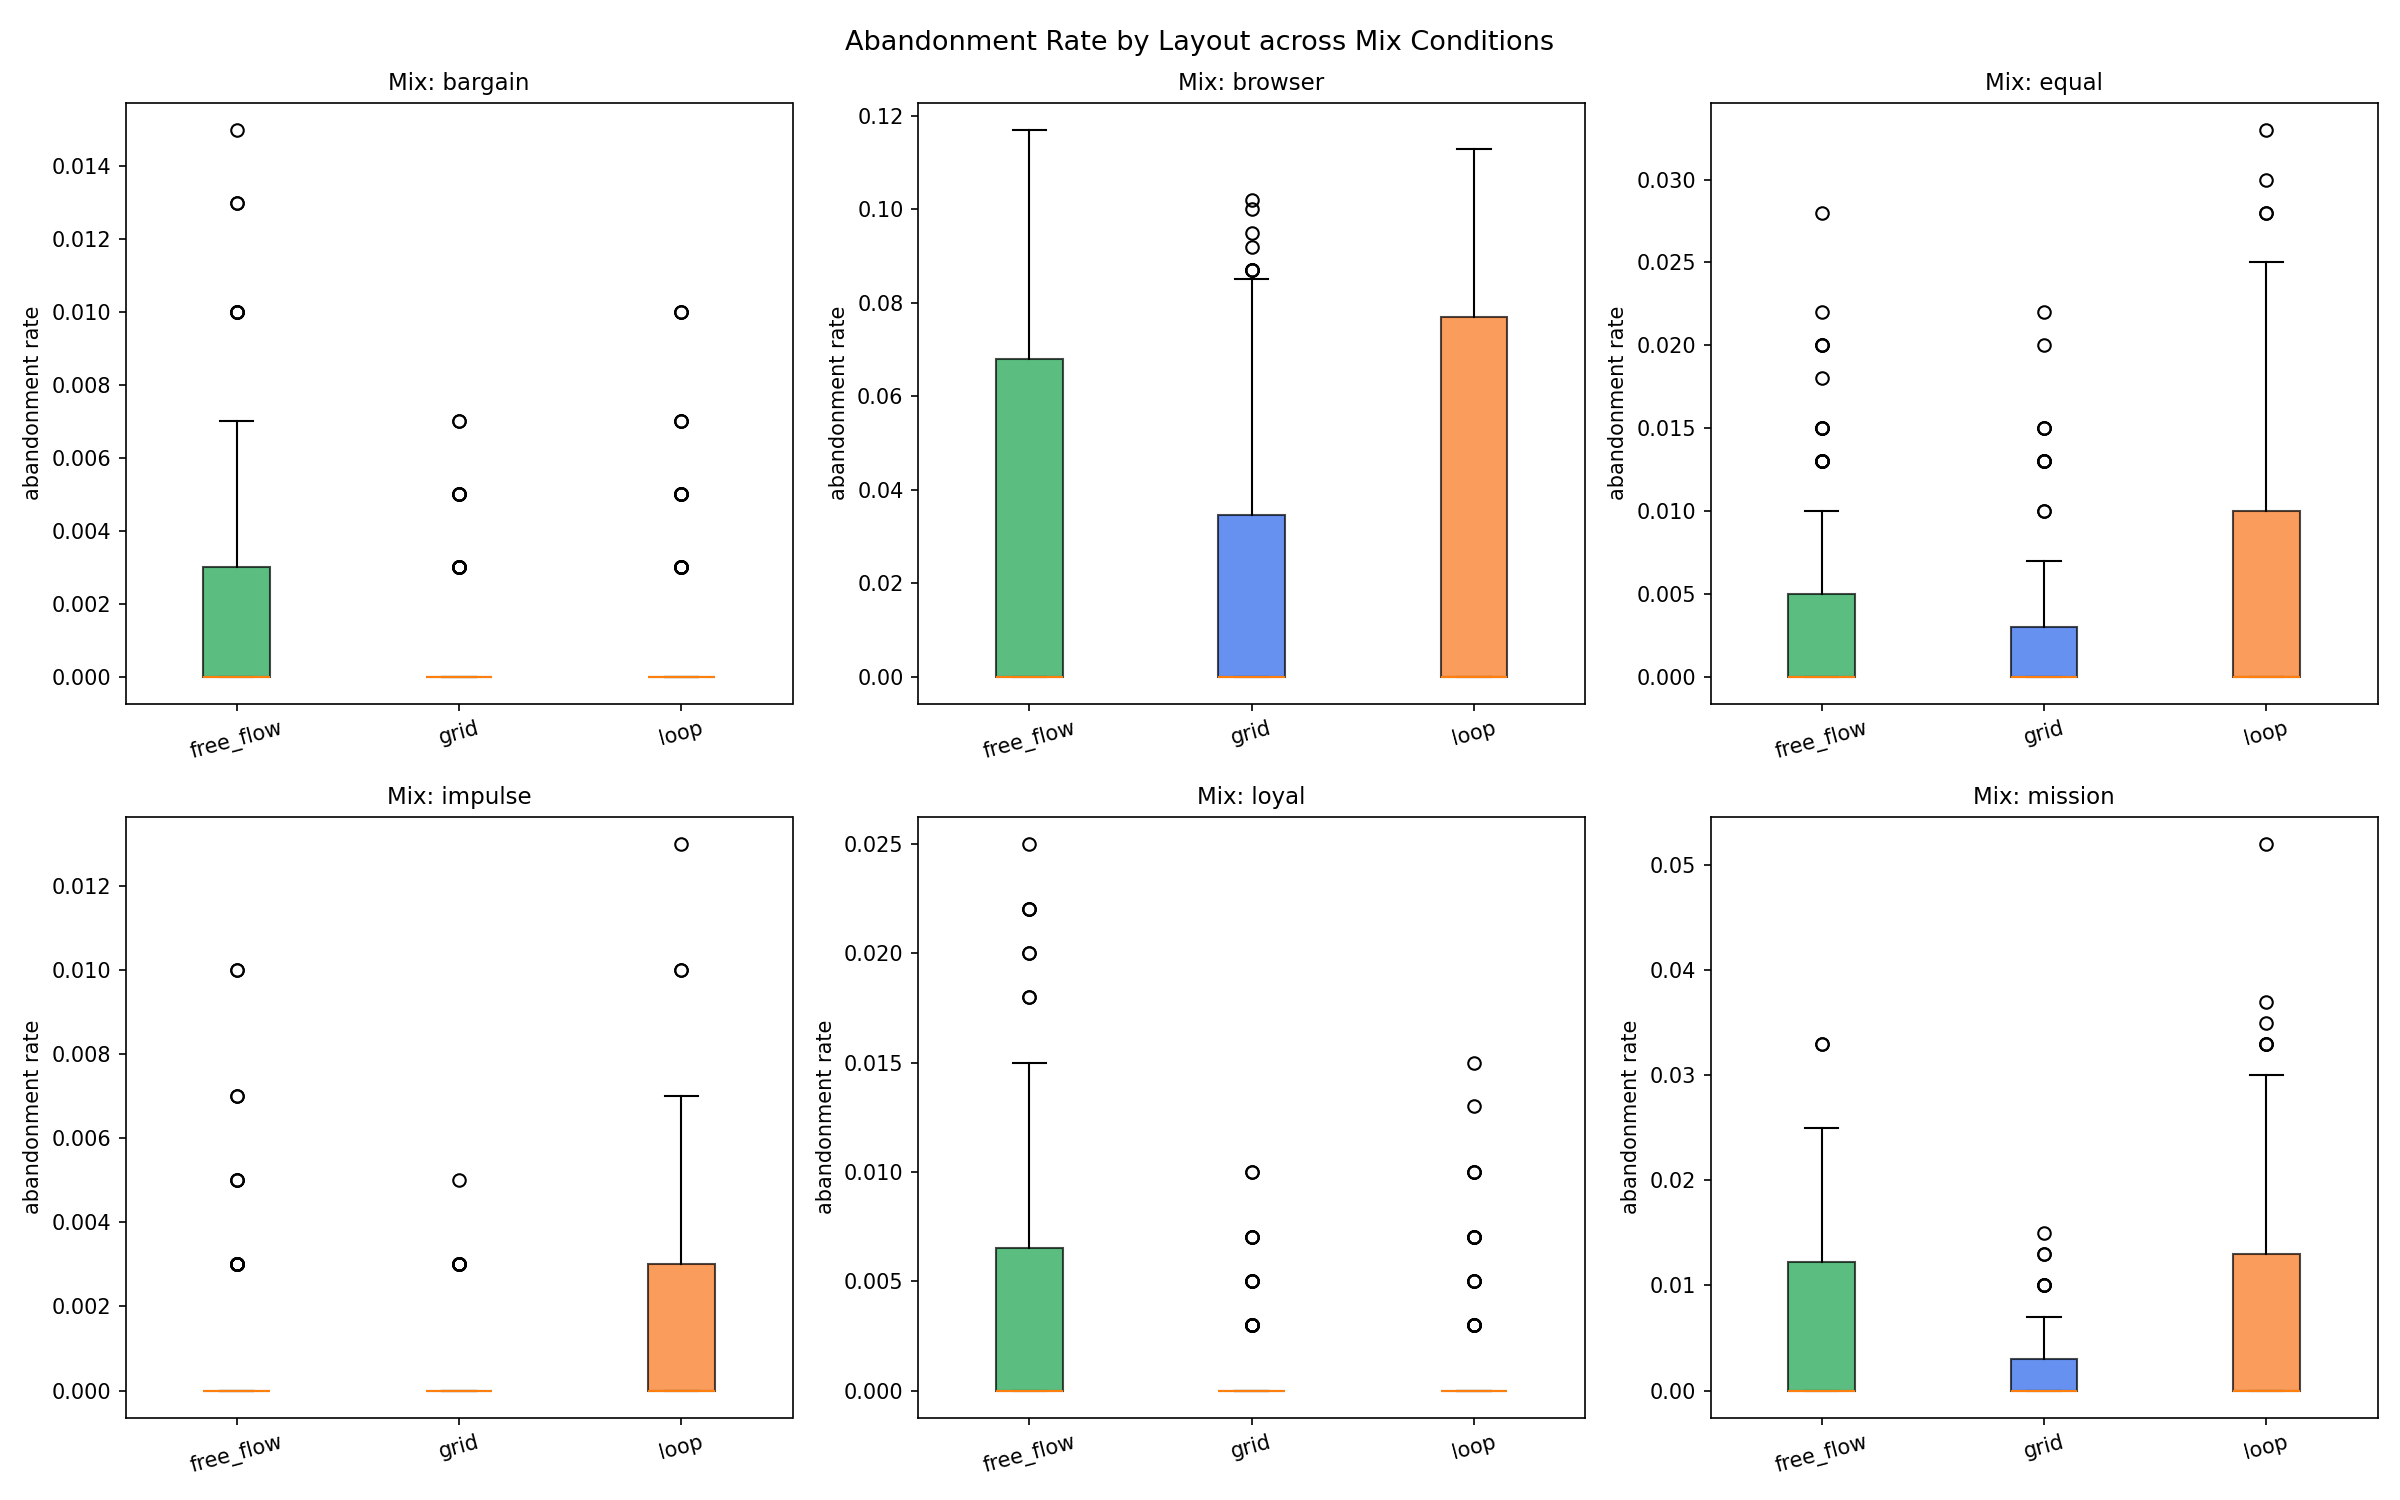
\includegraphics[width=0.82\columnwidth]{boxplot_abandonment_rate.png}
\caption{Abandonment rate by density, layout, and shopper mix. The line chart shows the density trend, while the boxplot summarizes run-level abandonment variation.}
\Description{Abandonment-rate line chart and boxplot for grid, loop, and free-flow layouts across shopper mixes.}
\label{fig:abandonment-rate}
\end{figure}

Figure~\ref{fig:abandonment-rate} shows that abandonment is primarily a high-density stress outcome. Browsers are most affected because they spend longer exploring, which exposes them to more crowding and checkout delay. This pattern is consistent with queueing research that treats abandonment as a consequence of waiting and impatience \citep{dai2013}, and with supermarket queue studies showing that checkout service and queue length are operationally meaningful \citep{mohamad2022,chandra2023}.

\subsection{Average Patience Drop}

Average patience drop measures how much frustration accumulated during the shopping trip. Grid produced the lowest patience drop in all six high-density mixes. The lowest grid patience drop was in the mission-driven mix at 53.9 minutes, while the highest was in the browser mix at 95.0 minutes. In the browser mix, patience drop reached 121.2 minutes in loop and 125.1 in free-flow.

\begin{figure}[t]
\centering
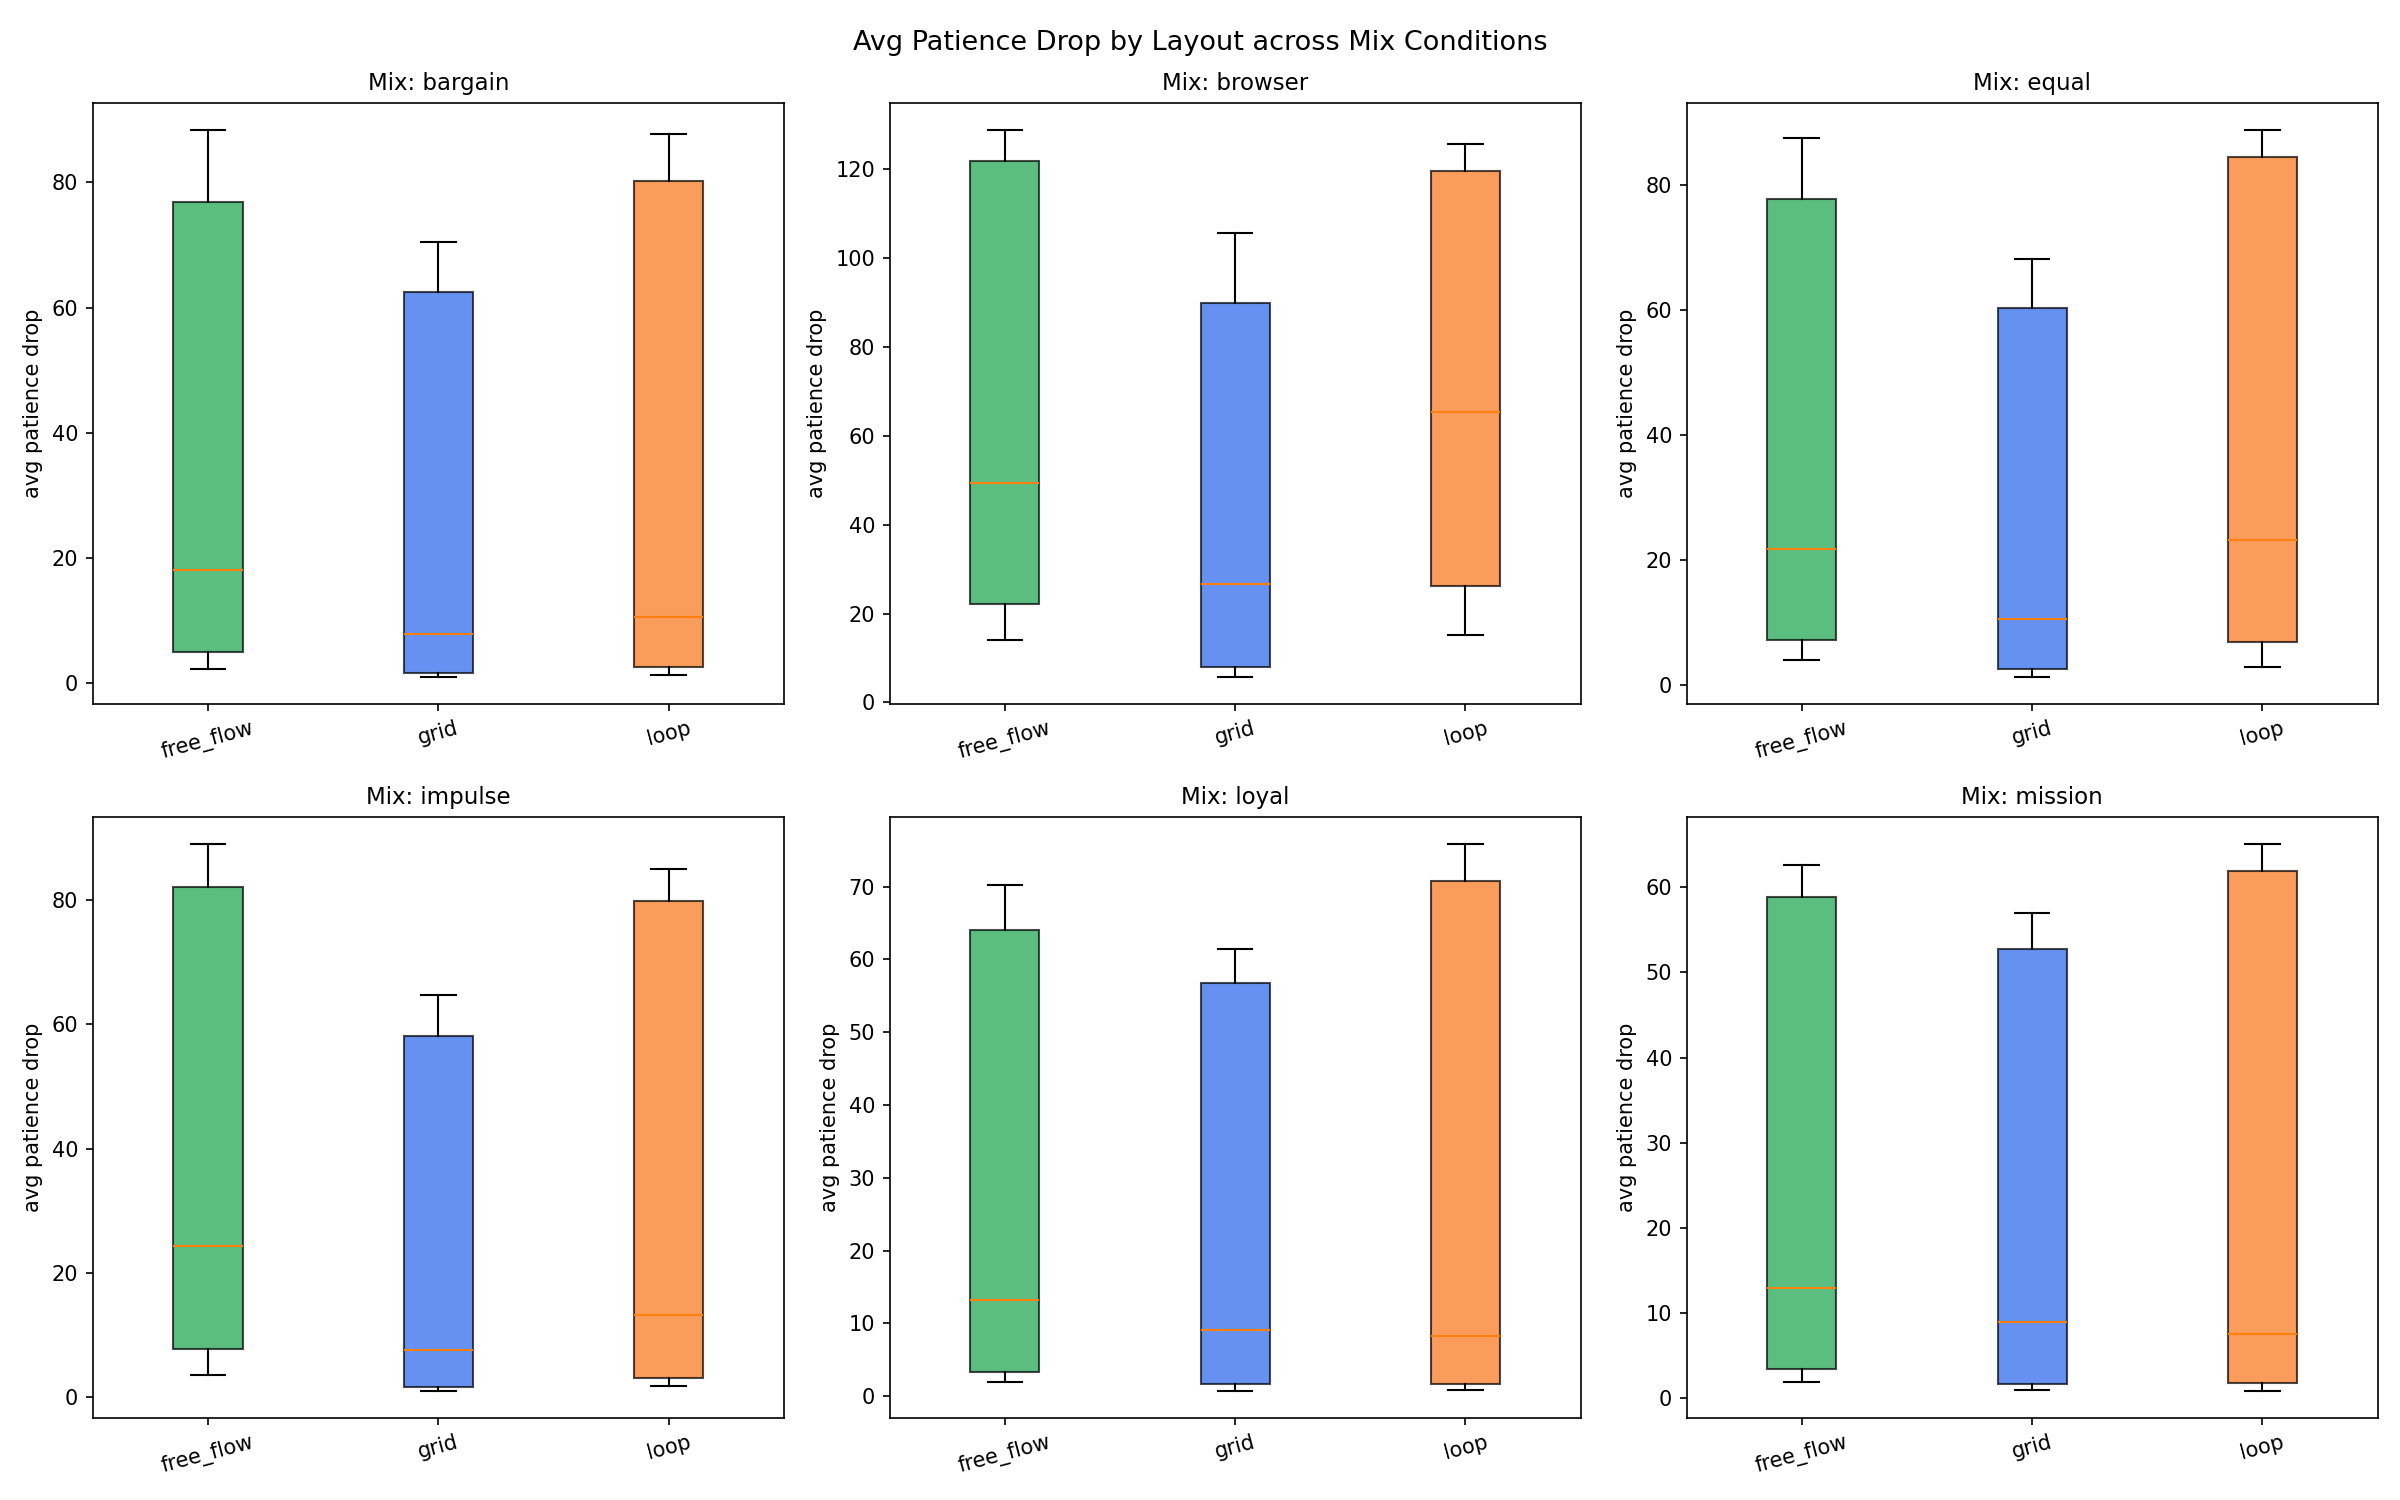
\includegraphics[width=0.90\columnwidth]{boxplot_avg_patience_drop.png}
\caption{Average patience drop by layout and shopper mix. The boxplot shows how much patience shoppers lost across simulation runs.}
\Description{Boxplot of average patience drop for grid, loop, and free-flow layouts across shopper mixes.}
\label{fig:patience-drop}
\end{figure}

Figure~\ref{fig:patience-drop} shows that patience loss is lowest in grid and higher in loop and free-flow. Loop increases exposure and list coverage, but that benefit comes with longer movement and more crowd encounters. Free-flow performs poorly because its exploratory paths increase uncertainty. These findings are consistent with retail-crowding research showing that crowding affects customer outcomes and perceived control \citep{blut2020}, basket composition \citep{aydinli2021}, and behavior near supermarket shelves \citep{luck2015}.

\subsection{Congestion Block Frequency}

Congestion block frequency measures how often shoppers were prevented from moving because local space was occupied. This metric is important because it connects layout geometry to behavioral outcomes. A layout can be attractive or exposure-rich, but if its paths create repeated blocking, shoppers lose patience and may leave before completing the trip.

\begin{figure}[t]
\centering
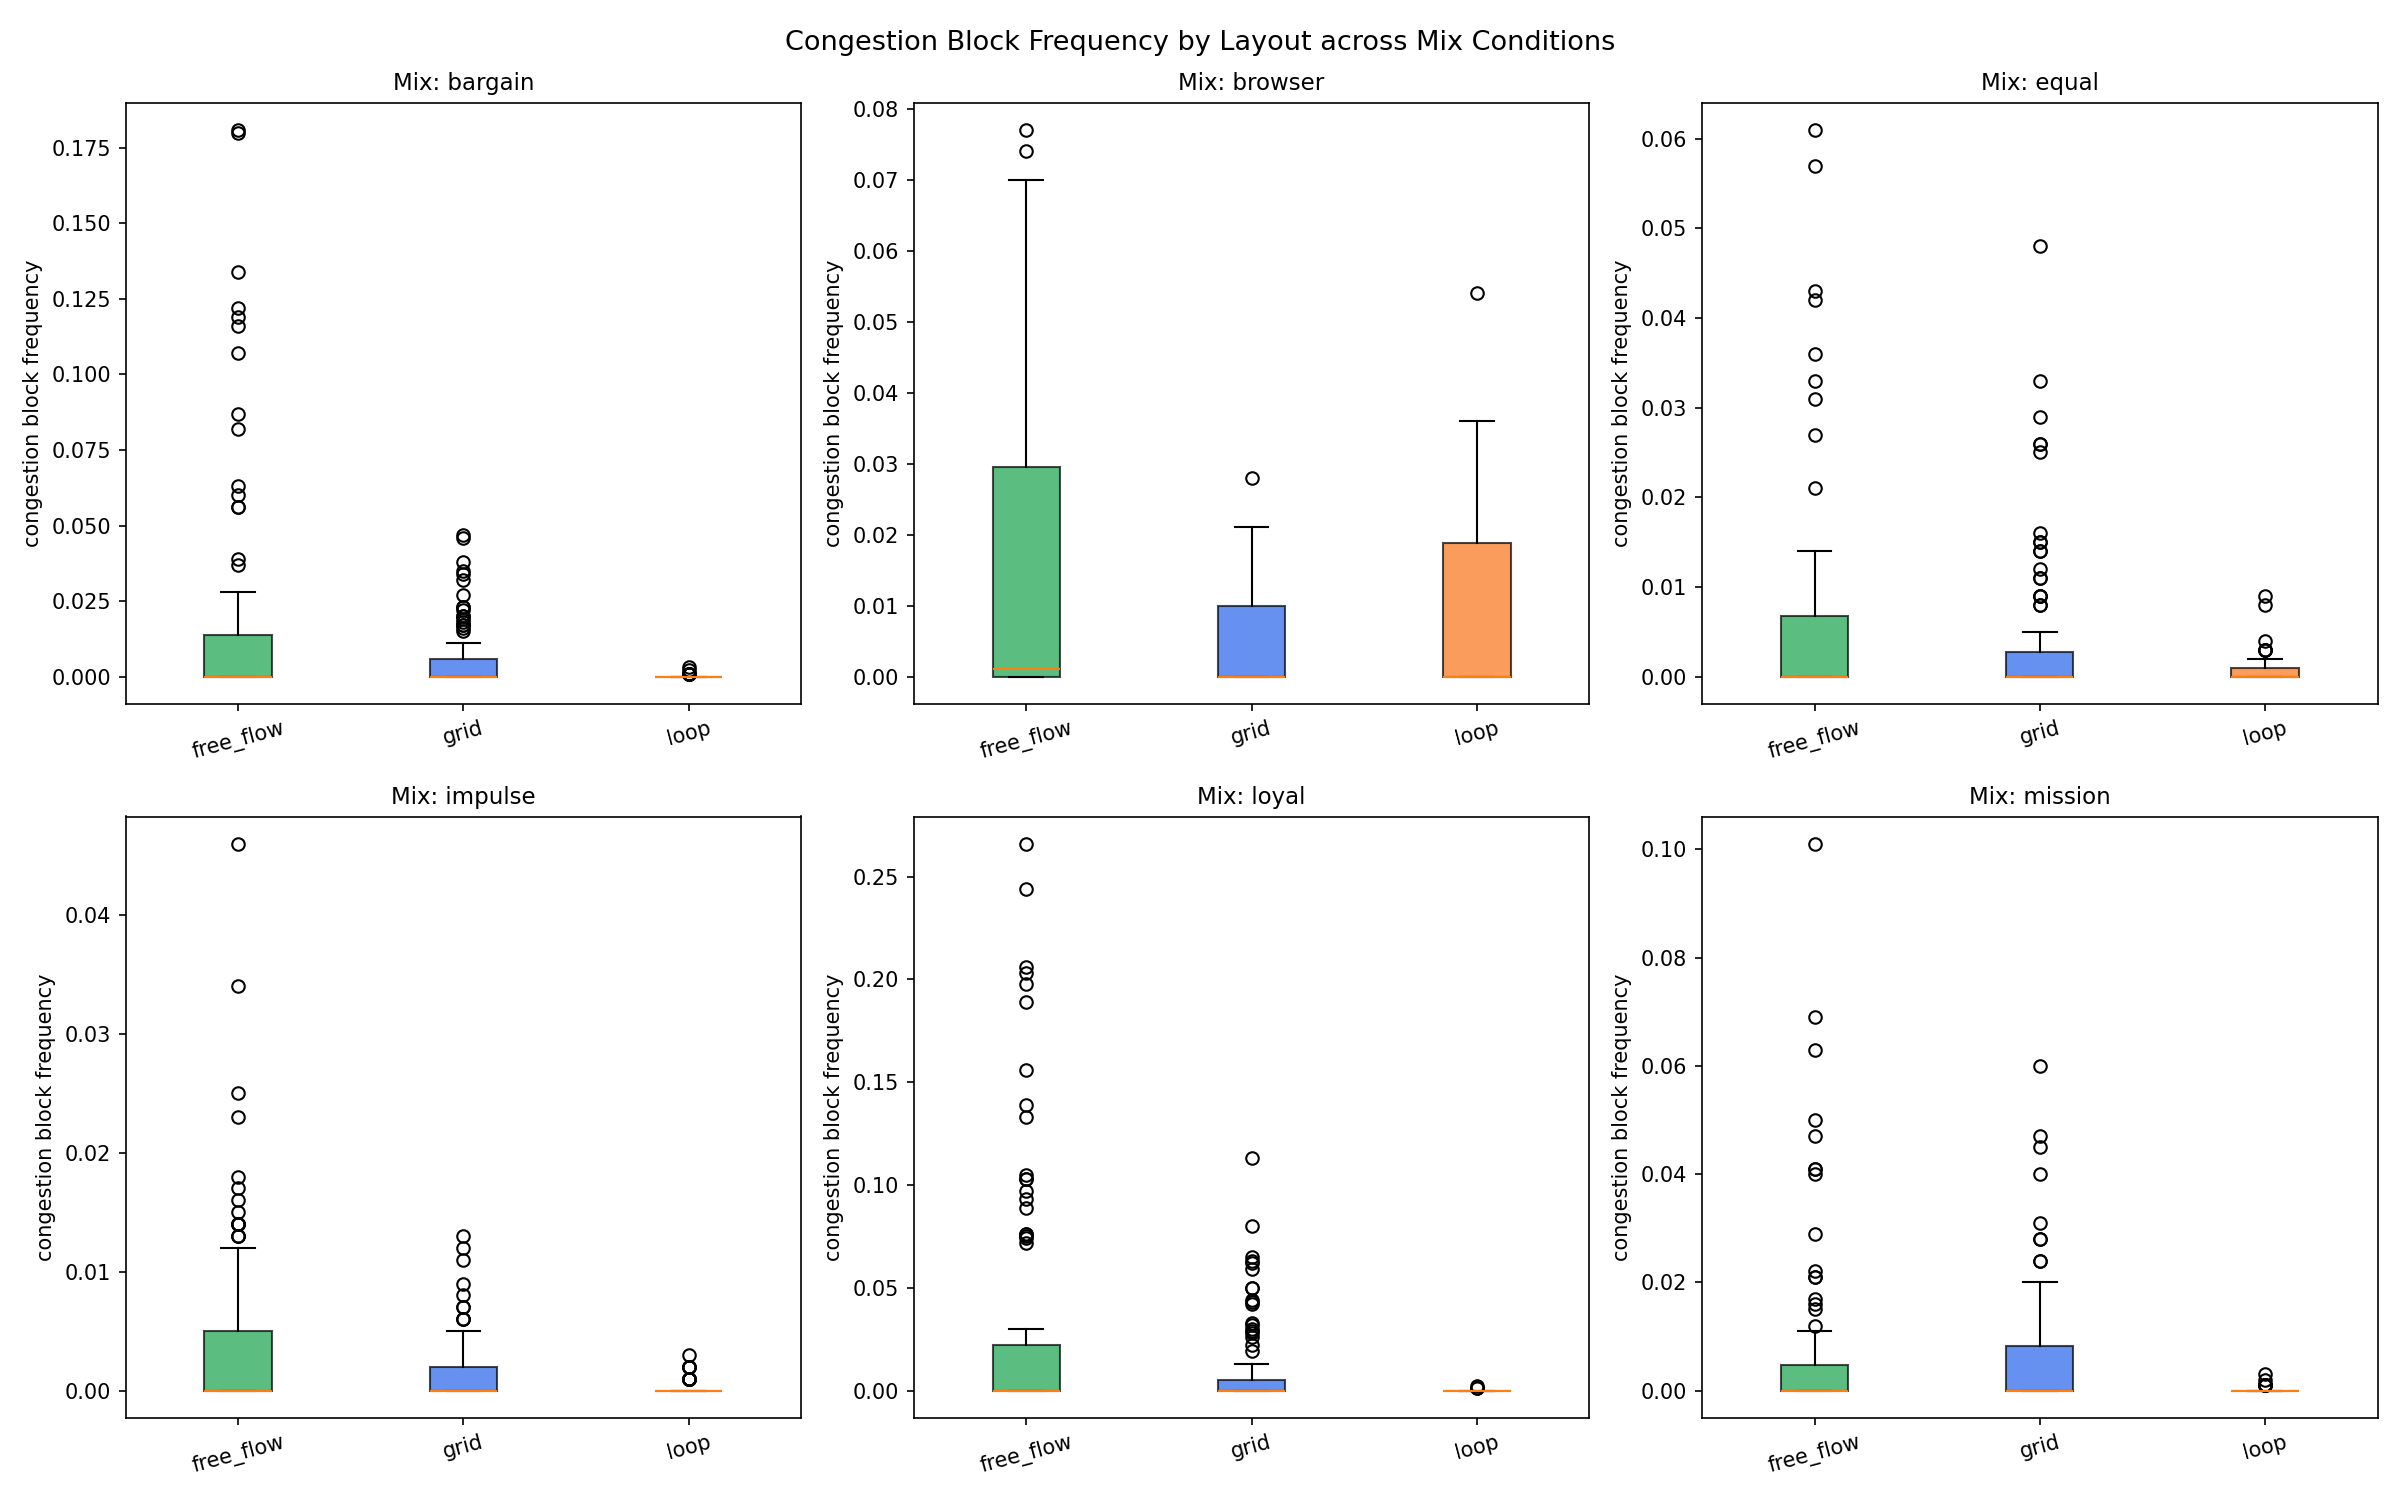
\includegraphics[width=0.90\columnwidth]{boxplot_congestion_block_frequency.png}
\caption{Congestion block frequency by layout and shopper mix. The boxplot summarizes how often shoppers experienced blocked movement during simulation runs.}
\Description{Boxplot of congestion block frequency for grid, loop, and free-flow layouts across shopper mixes.}
\label{fig:congestion-frequency}
\end{figure}

Figure~\ref{fig:congestion-frequency} shows that congestion is not evenly distributed across layouts. Grid reduces blocking because its structured aisles create clearer movement channels. Loop and free-flow expose shoppers to more shared-path conflict, especially under high density. This supports the model's treatment of congestion as a mechanism linking store layout to patience loss, completion, and abandonment \citep{blut2020,pantano2021}.

\subsection{Completed-versus-Abandoned Chi-Square Tests}

The chi-square tests evaluate whether the distribution of completed and abandoned trips differs by layout. These tests were significant for all six shopper mixes, including the high-density condition. This provides categorical evidence that layout changes trip outcomes, not only average trip time or average purchasing totals.

\begin{figure}[t]
\centering
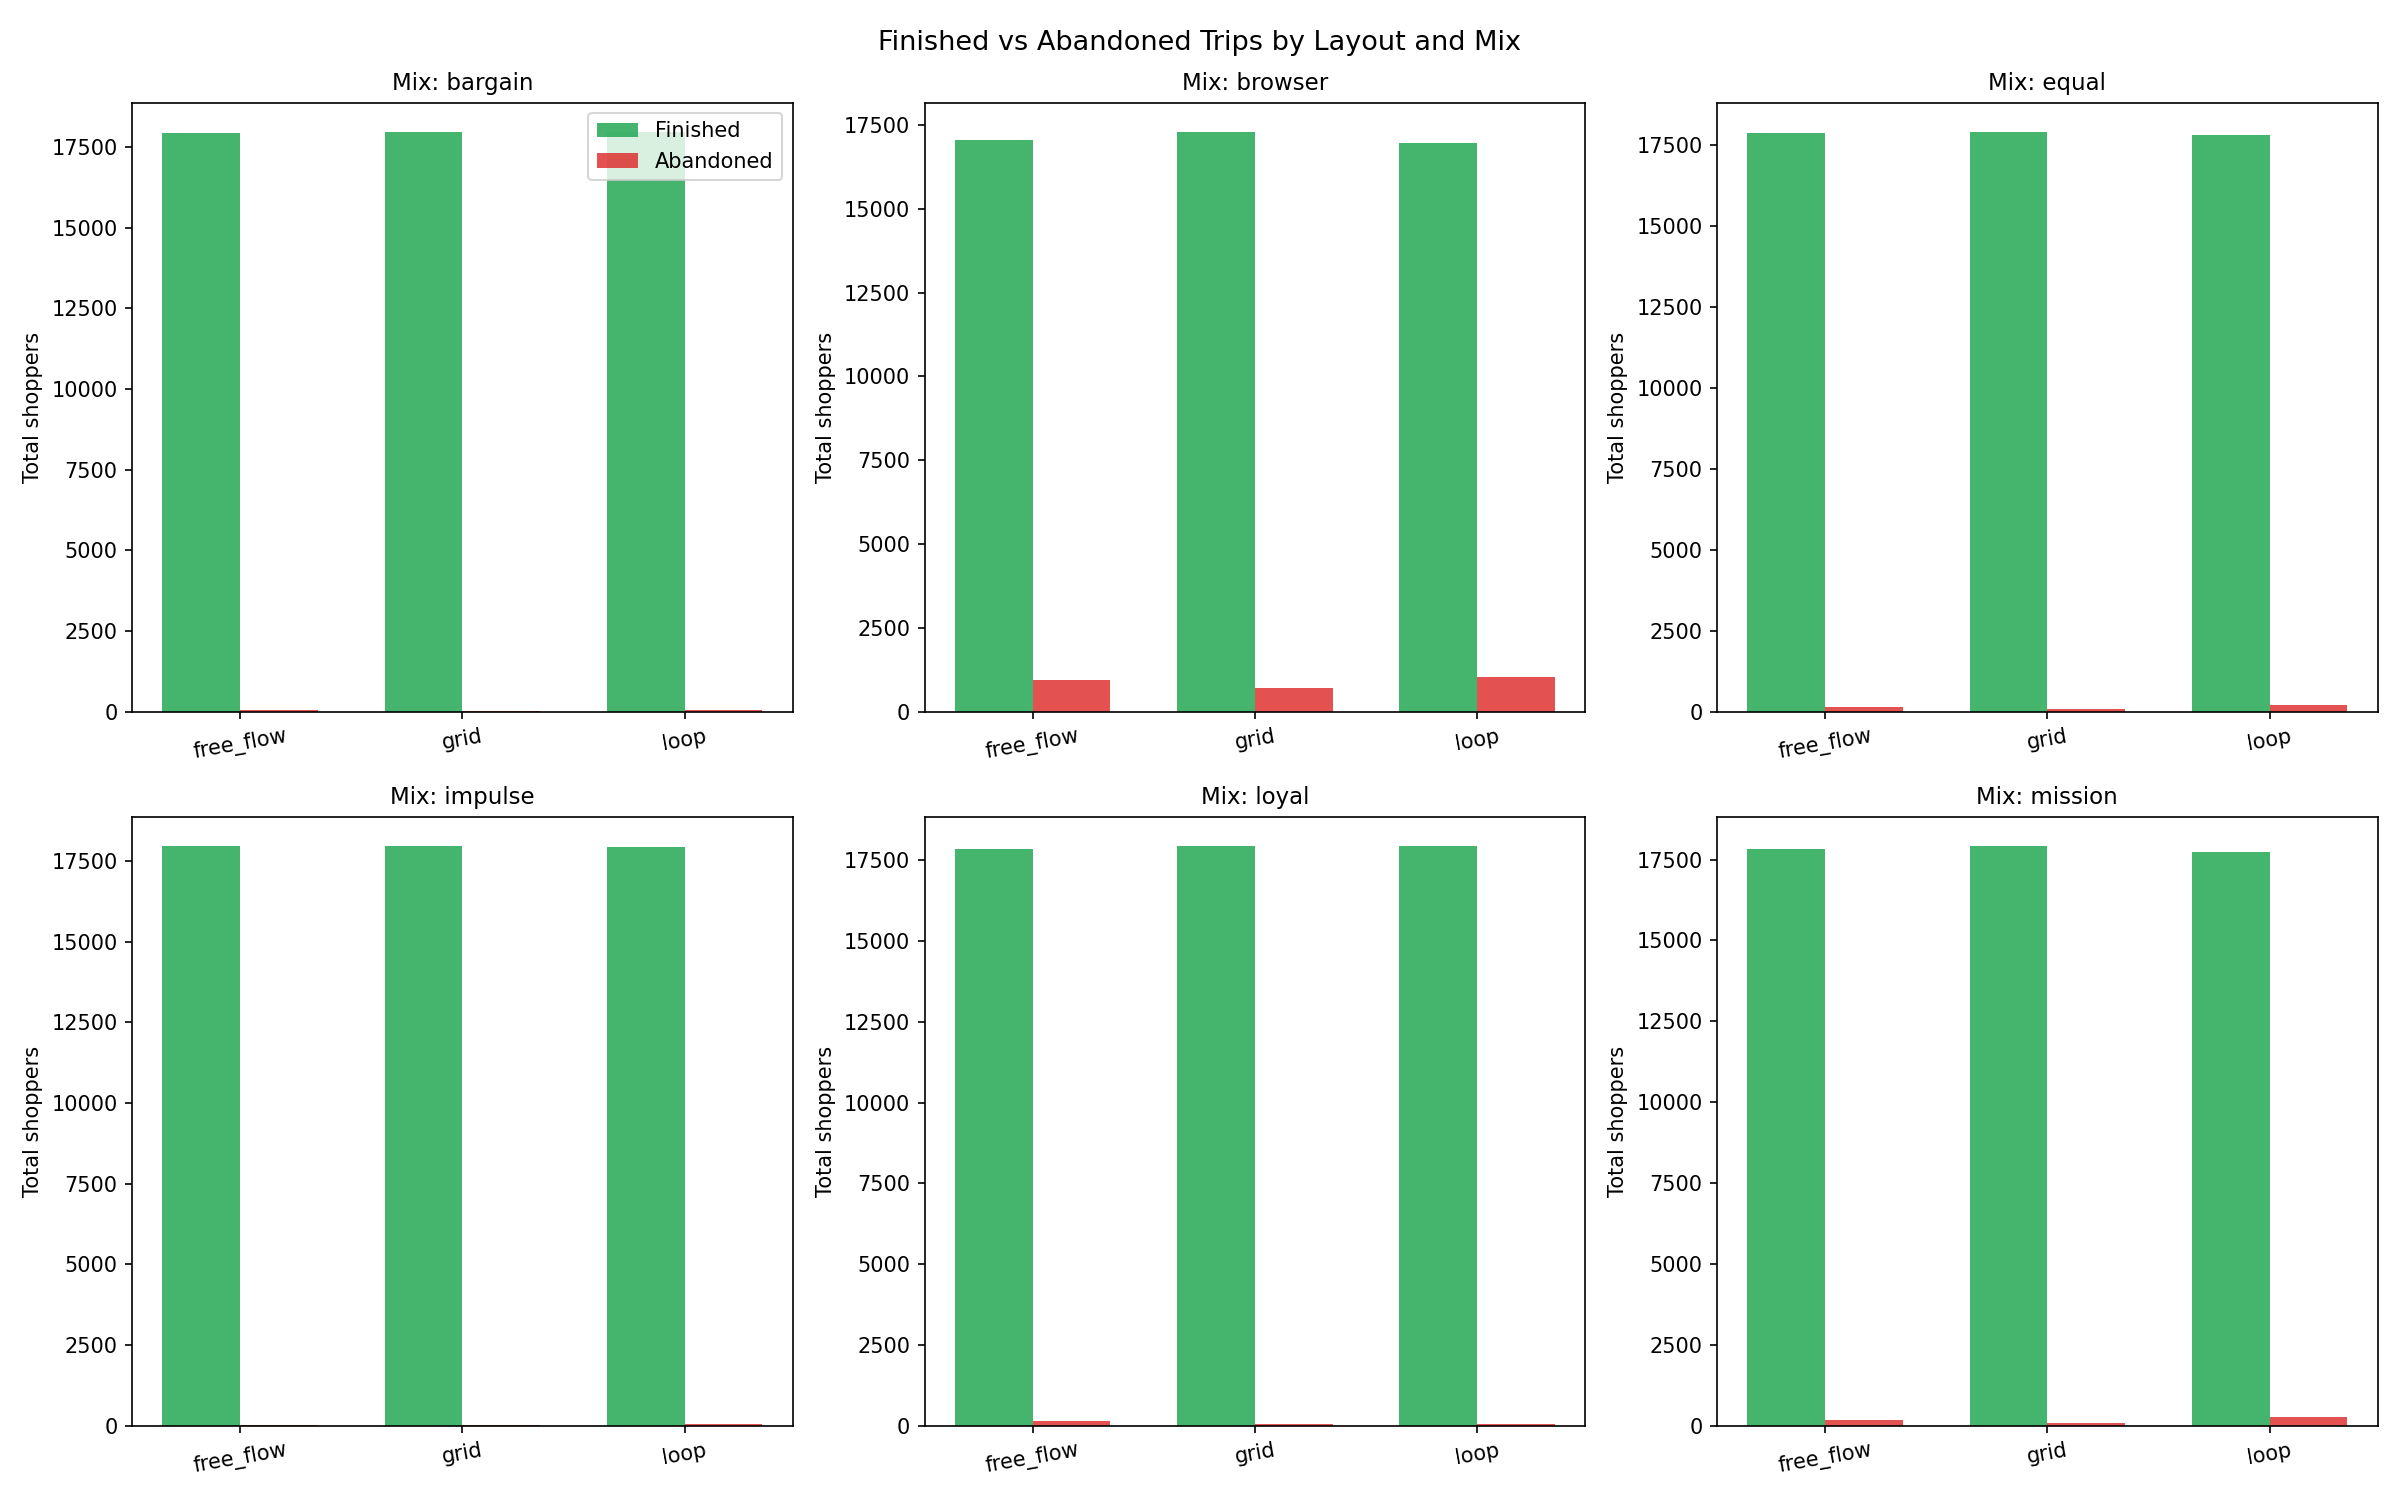
\includegraphics[width=0.95\columnwidth]{chisquare_bar.png}
\vspace{0.12in}
\begin{minipage}{0.48\columnwidth}
    \centering
    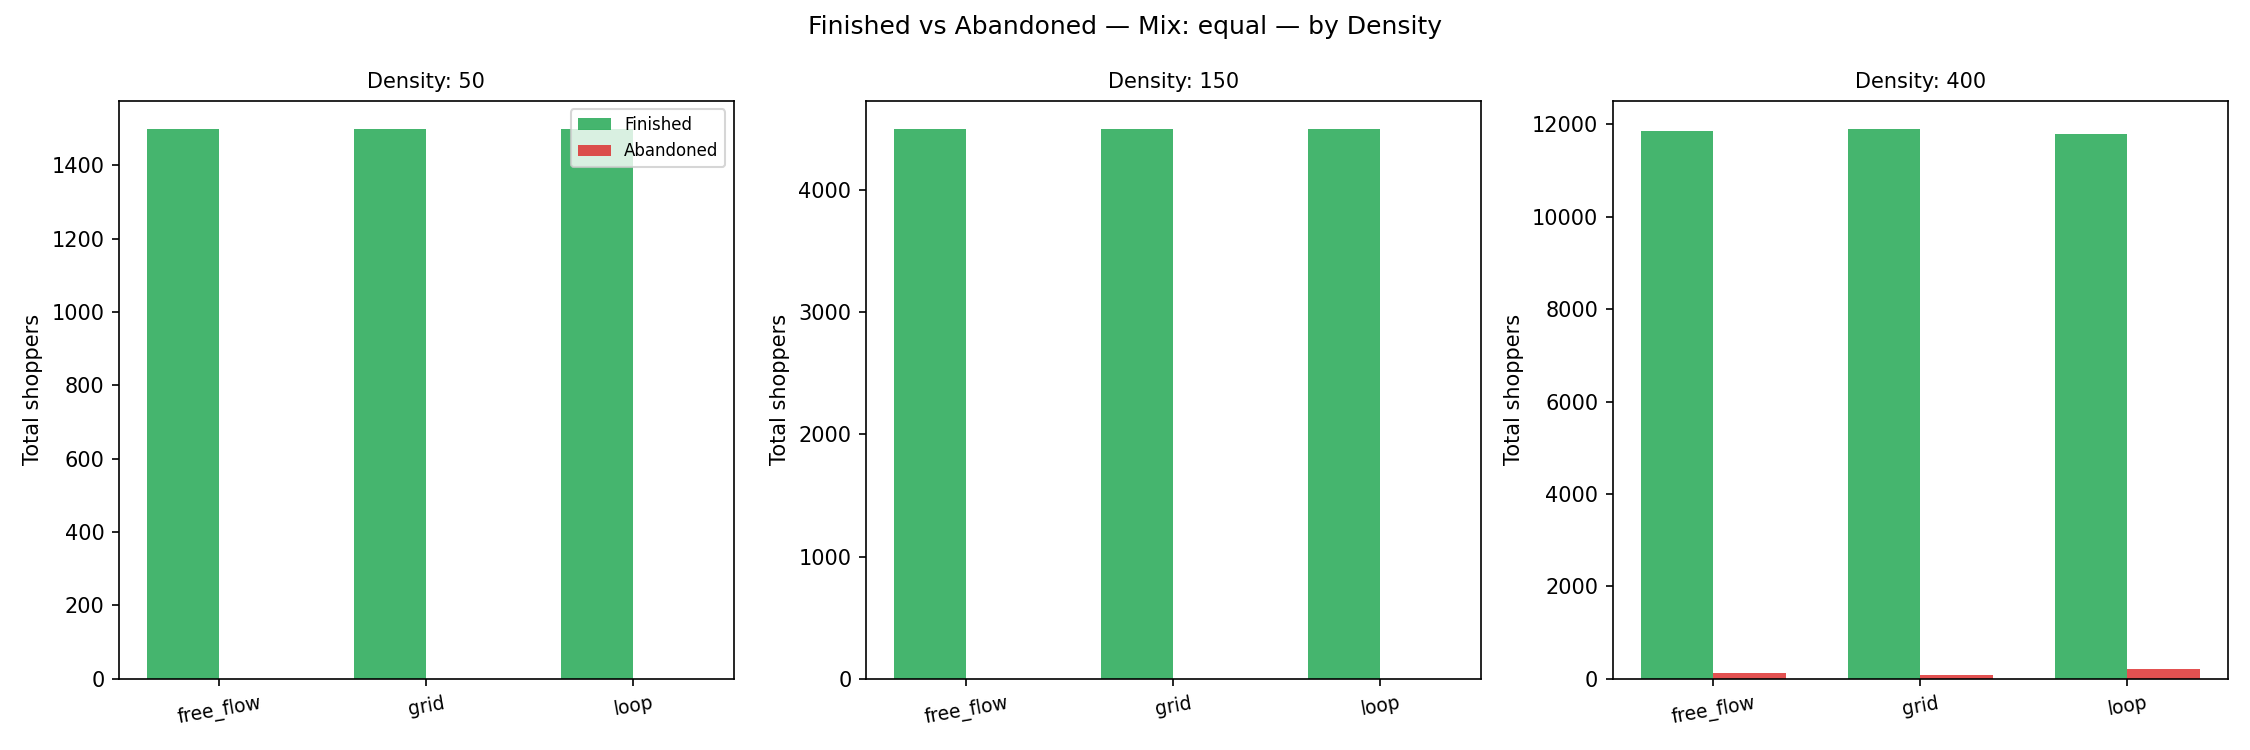
\includegraphics[width=\linewidth]{chisquare_density_equal.png}
\end{minipage}
\hfill
\begin{minipage}{0.48\columnwidth}
    \centering
    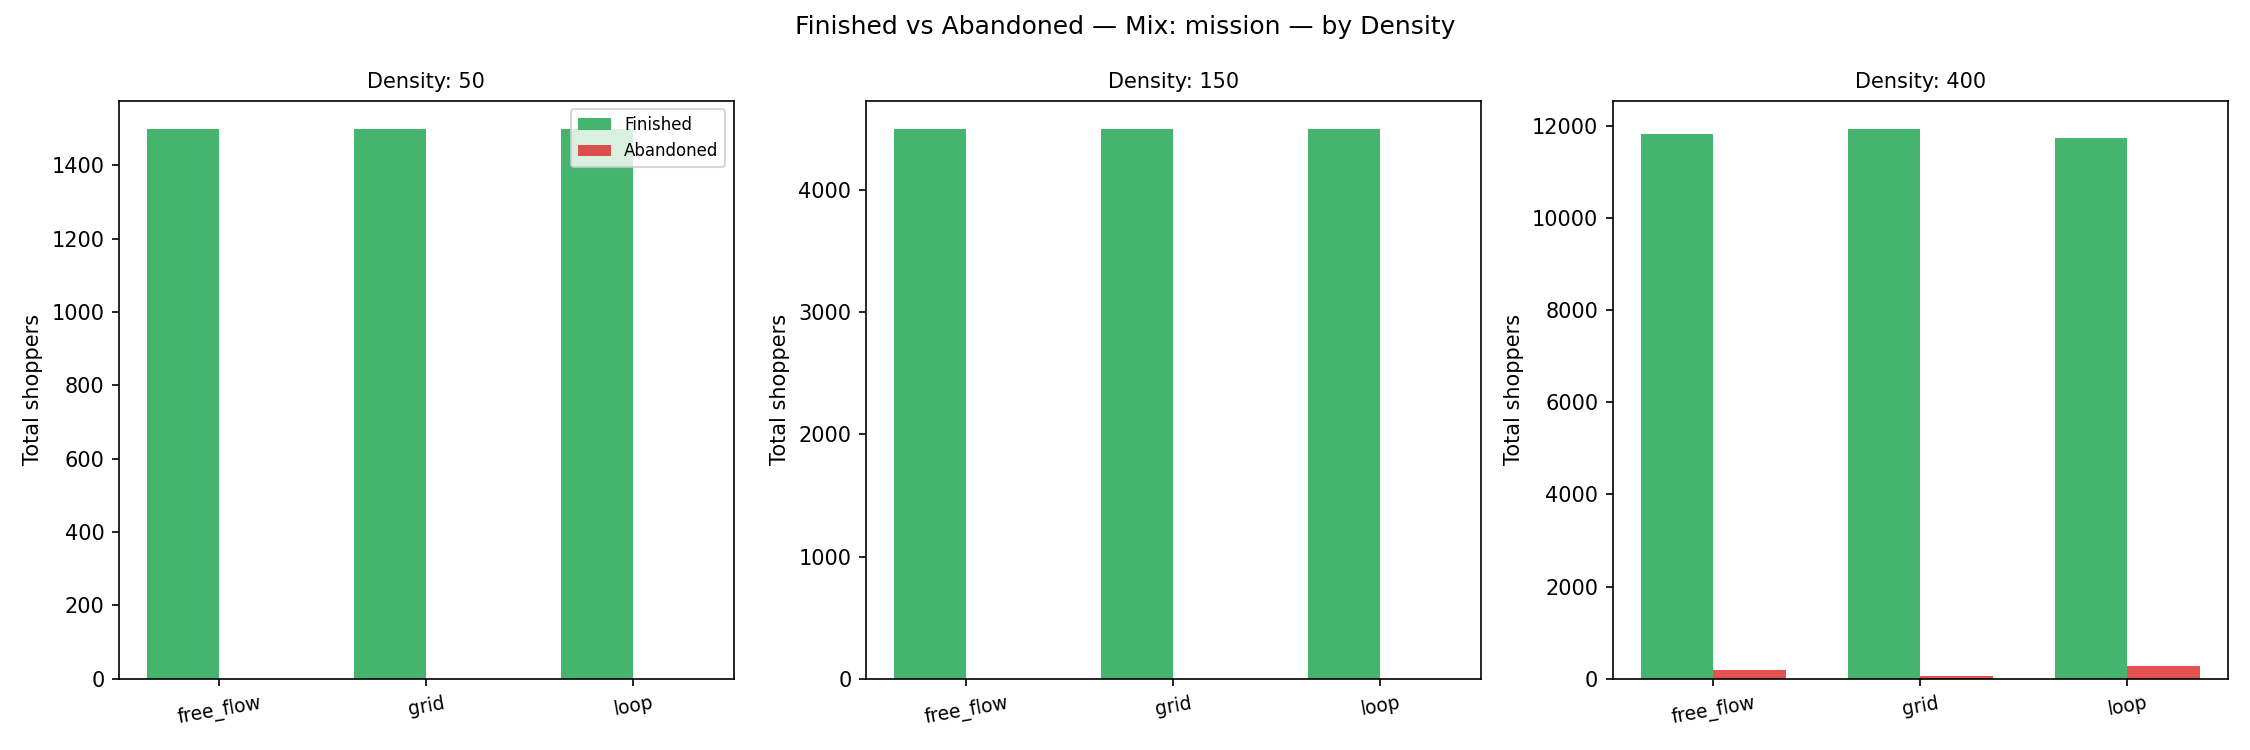
\includegraphics[width=\linewidth]{chisquare_density_mission.png}
\end{minipage}
\vspace{0.08in}
\begin{minipage}{0.48\columnwidth}
    \centering
    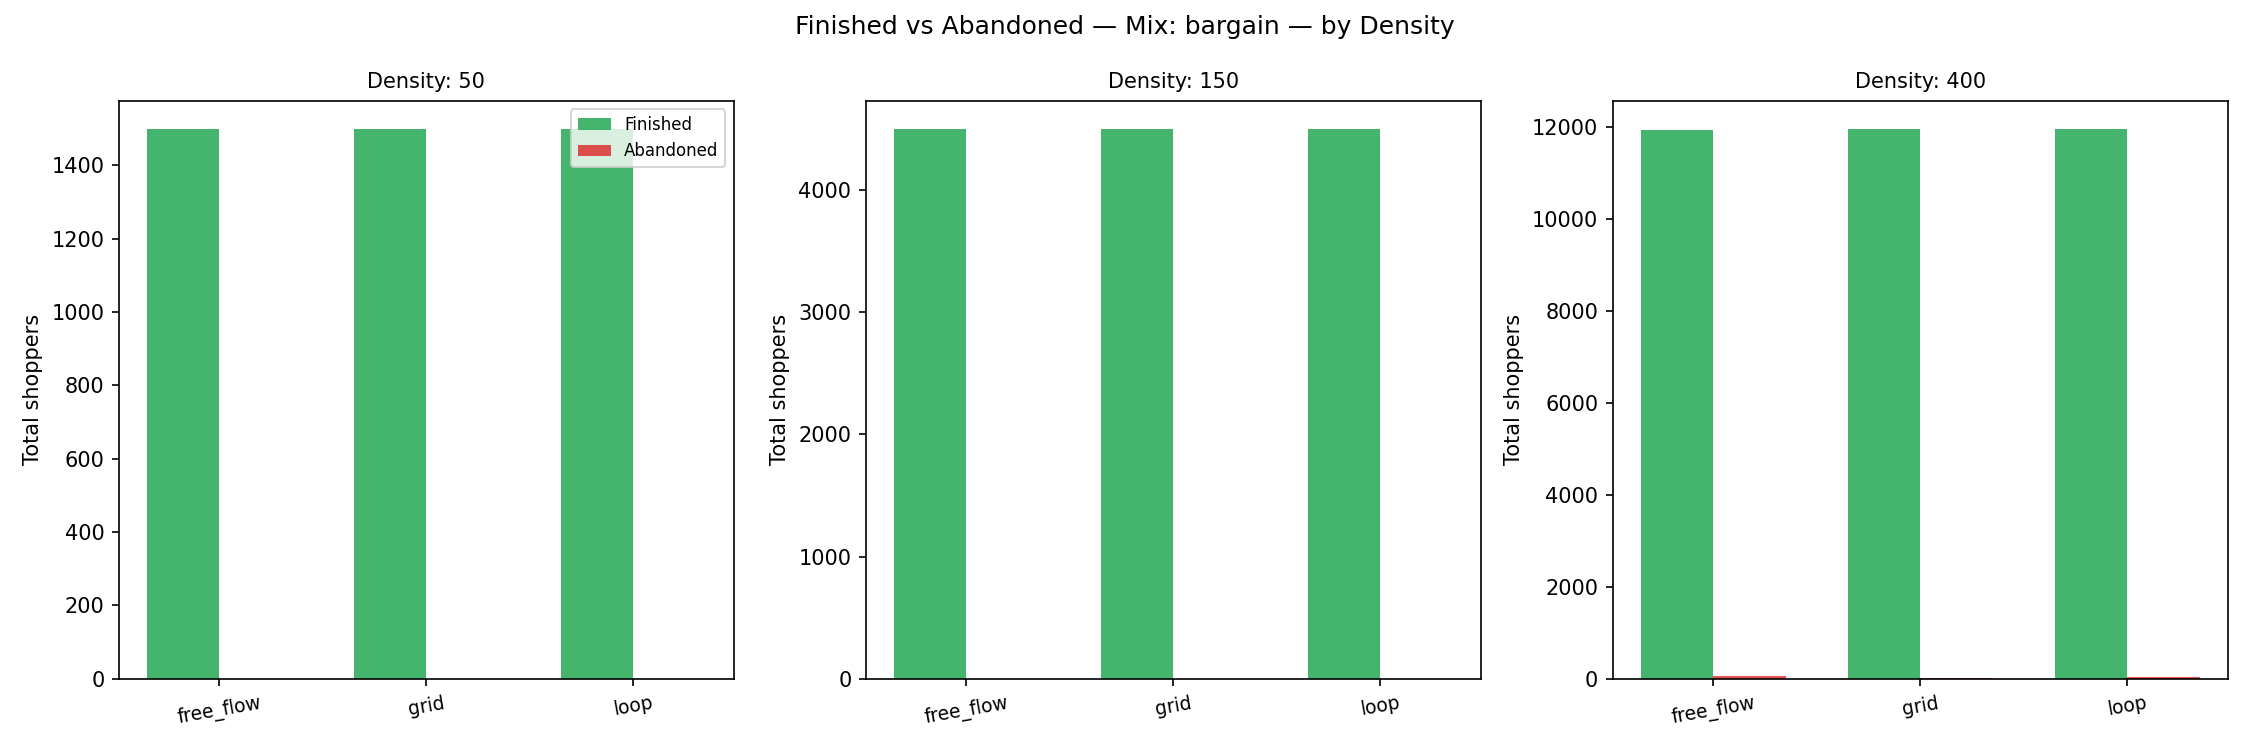
\includegraphics[width=\linewidth]{chisquare_density_bargain.png}
\end{minipage}
\hfill
\begin{minipage}{0.48\columnwidth}
    \centering
    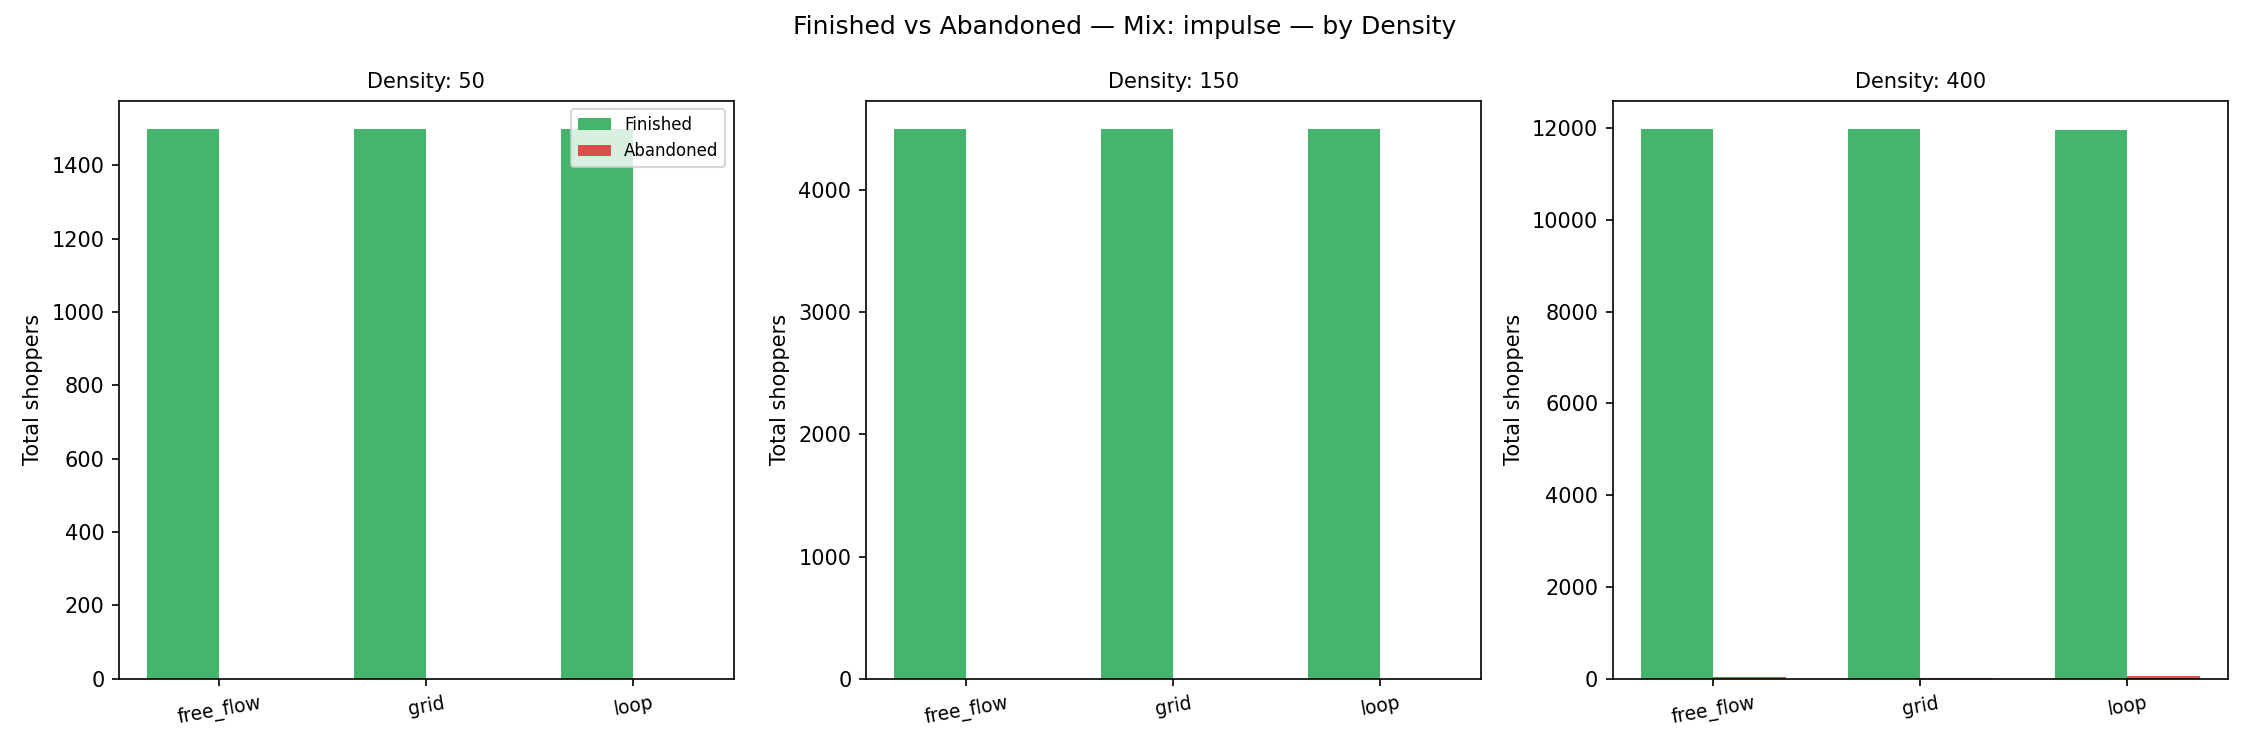
\includegraphics[width=\linewidth]{chisquare_density_impulse.png}
\end{minipage}
\vspace{0.08in}
\begin{minipage}{0.48\columnwidth}
    \centering
    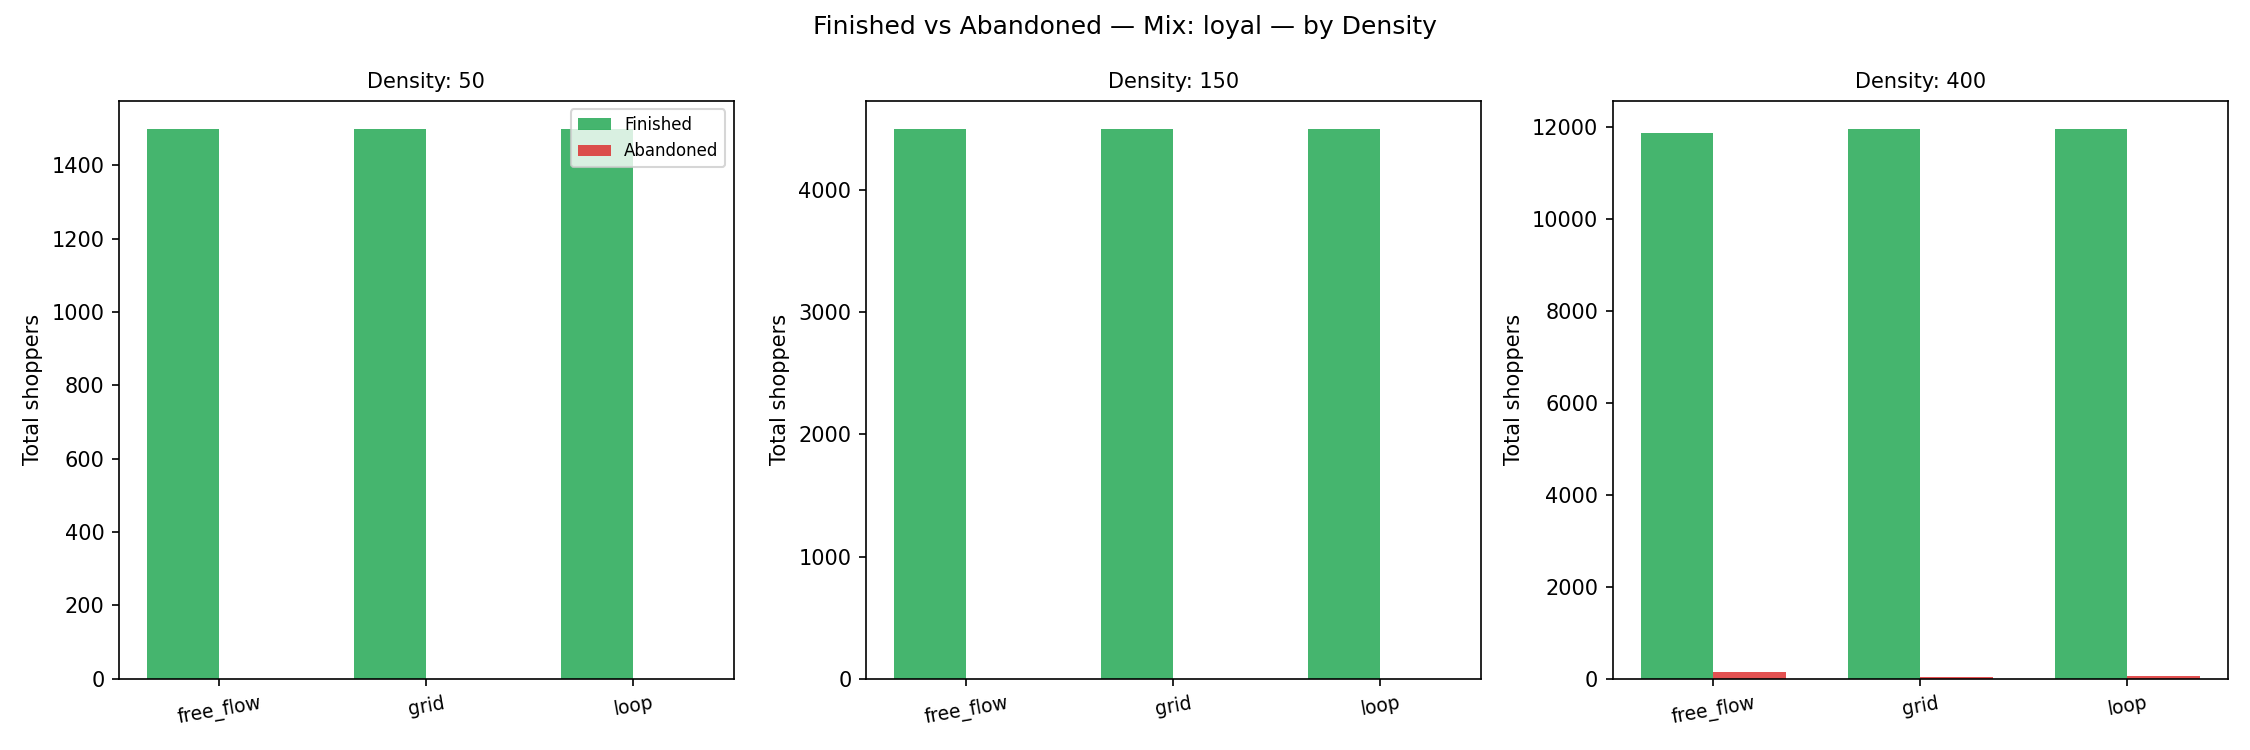
\includegraphics[width=\linewidth]{chisquare_density_loyal.png}
\end{minipage}
\hfill
\begin{minipage}{0.48\columnwidth}
    \centering
    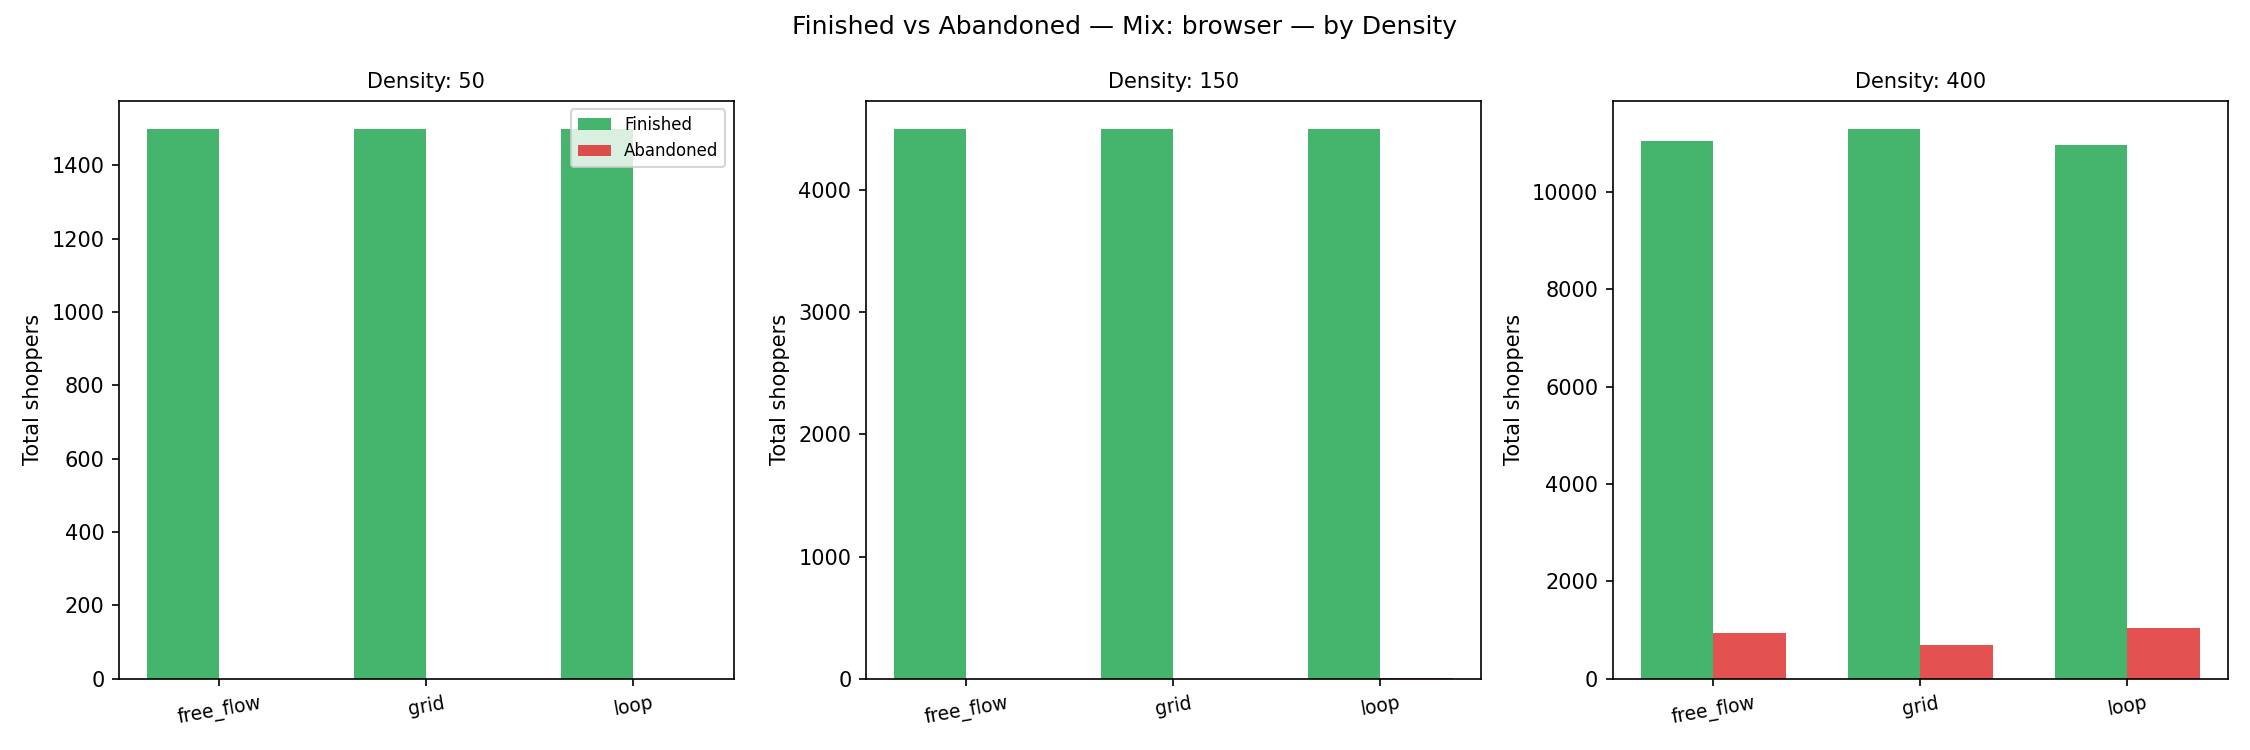
\includegraphics[width=\linewidth]{chisquare_density_browser.png}
\end{minipage}
\caption{Chi-square results for completed versus abandoned trips. The top panel summarizes overall chi-square evidence by shopper mix, while the lower six panels show density-stratified chi-square results for each mix.}
\Description{Overall and density-stratified chi-square plots for completed versus abandoned trips across six shopper mixes.}
\label{fig:chisquare-tests}
\end{figure}

Figure~\ref{fig:chisquare-tests} supports the rejection of the null hypothesis for trip completion outcomes. The density-stratified panels show that the completed-versus-abandoned difference becomes most important at high density, where shoppers compete for aisle and checkout space. This aligns with queueing theory, where abandonment is a standard result of delay and impatience \citep{dai2013}, and with supermarket queue studies that treat queue length and service rate as important operational concerns \citep{mohamad2022,chandra2023}.

\subsection{Spearman Correlation Heatmap}

The Spearman heatmap shows how the simulation outcomes relate to each other across the final result set. Congestion block frequency was strongly associated with patience drop ($r_s=0.704$) and moderately associated with items not found ($r_s=0.466$). Patience drop was also strongly associated with abandonment rate ($r_s=0.727$).

\begin{figure}[t]
\centering
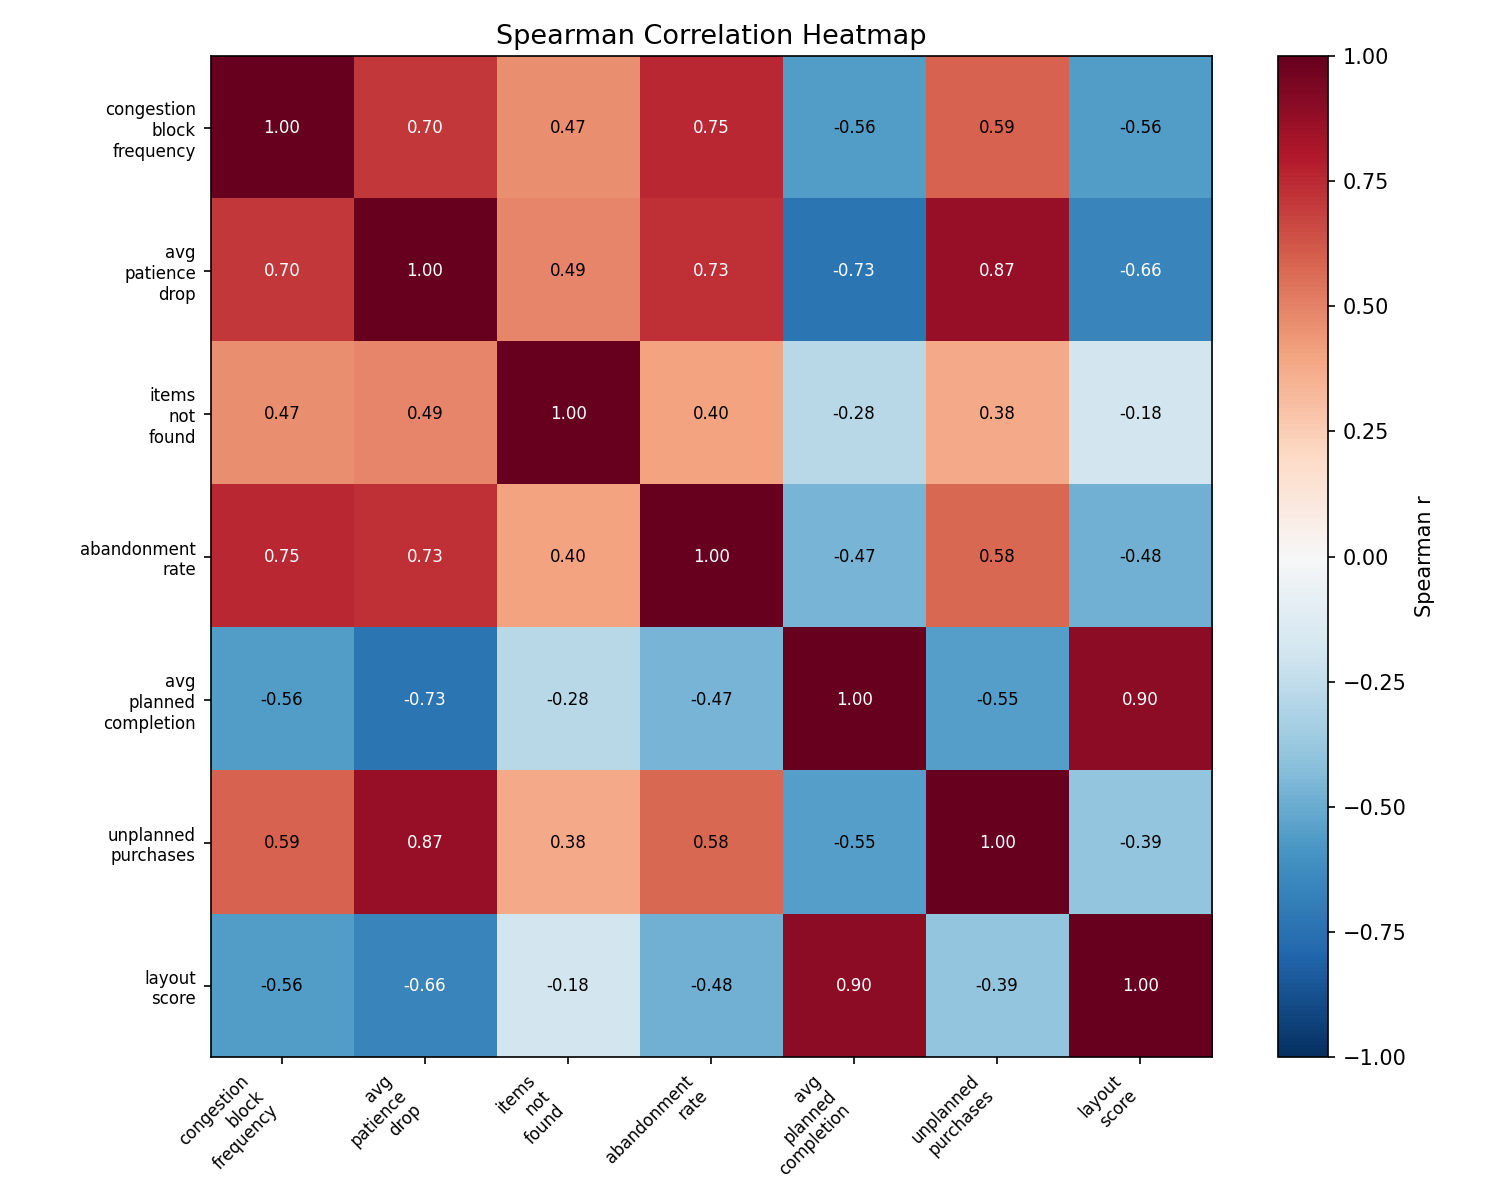
\includegraphics[width=\columnwidth]{correlation_heatmap.png}
\caption{Spearman correlation heatmap for final simulation outcomes. The heatmap shows relationships among congestion, patience drop, abandonment, list completion, missed items, purchasing, and layout score.}
\Description{Correlation heatmap linking congestion, patience loss, abandonment, planned completion, items not found, unplanned purchases, and layout score.}
\label{fig:correlation-heatmap}
\end{figure}

Figure~\ref{fig:correlation-heatmap} supports the causal interpretation used in the discussion: layout affects movement and congestion, congestion affects patience, and patience loss is associated with abandonment. The heatmap does not prove causality by itself, but it is consistent with retail-crowding literature showing that crowded store conditions affect customer experience and behavior \citep{blut2020,aydinli2021,luck2015}.

\subsection{Overall Layout Score}

Layout score is the weighted composite of planned completion, completed trips, unplanned purchases, abandonment, satisfaction, and congestion. Loop produced the highest layout score in five high-density mixes: equal, mission-driven, bargain-hunter, impulse-buyer, and loyal-shopper. The strongest high-density loop score was in the loyal-shopper mix at 93.9, followed by bargain-hunter at 92.9, impulse-buyer at 91.7, equal at 91.1, and mission-driven at 90.8. Browser was the exception: grid scored highest at 55.1, compared with 53.9 for free-flow and 53.4 for loop.

\begin{figure}[t]
\centering
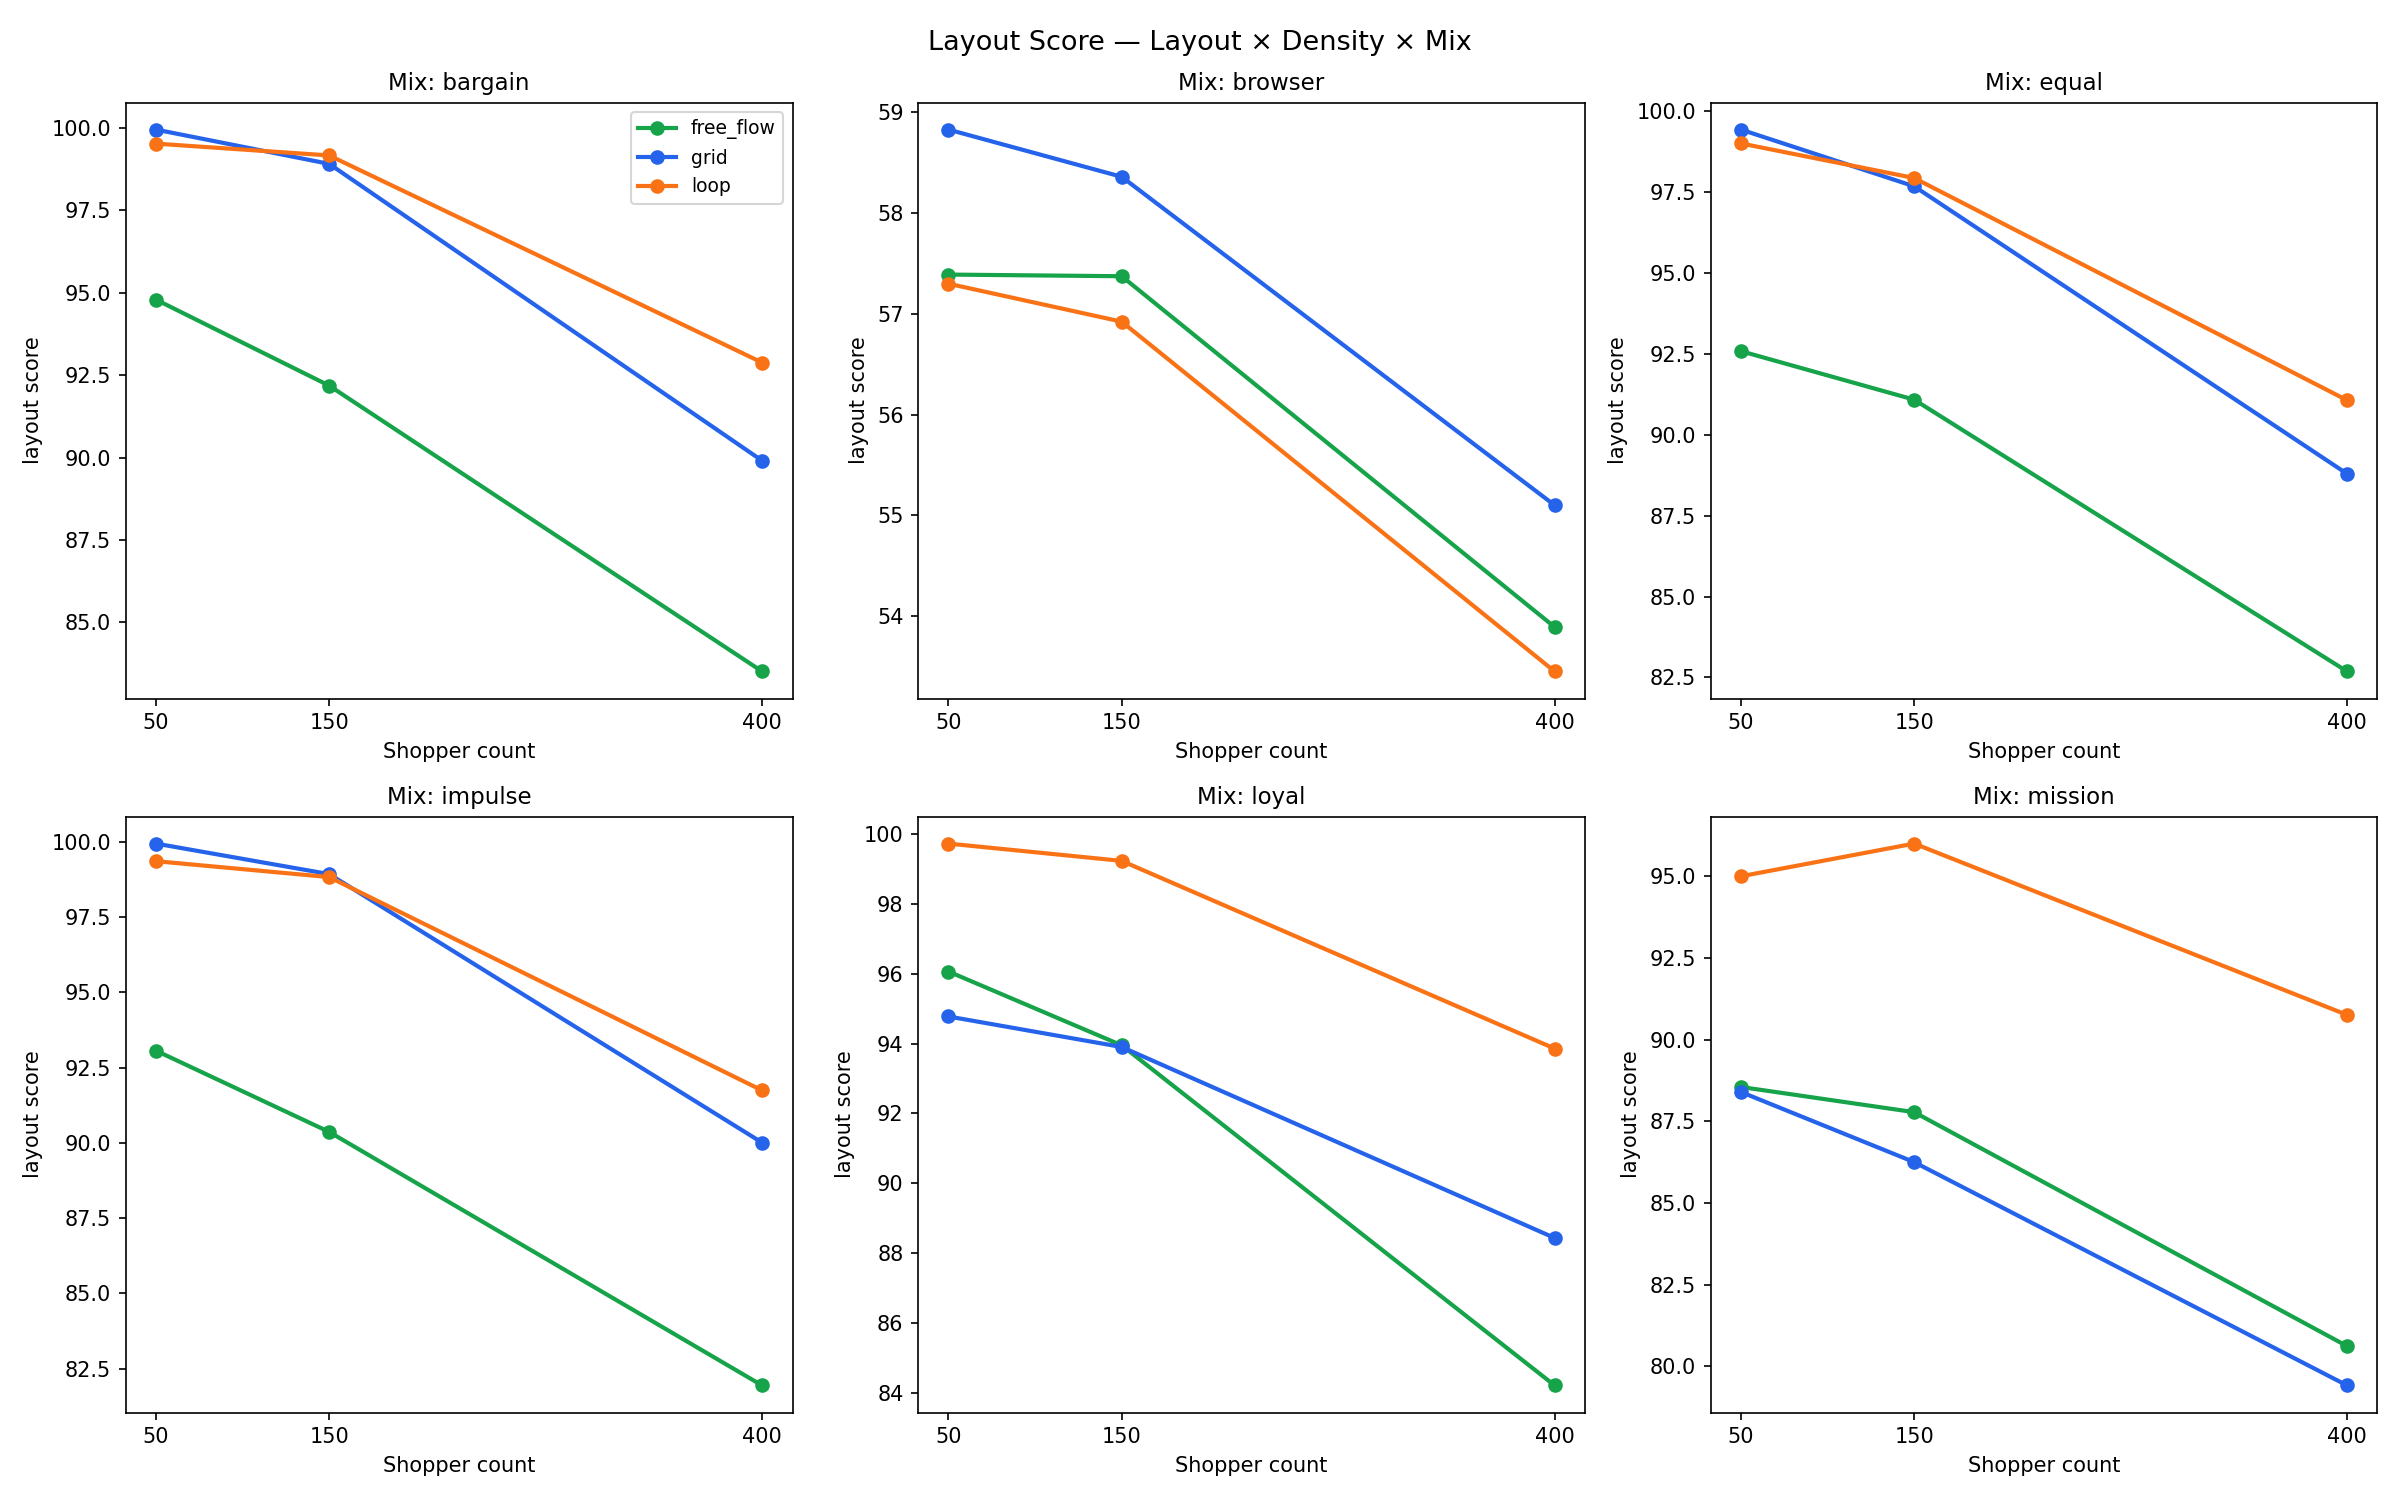
\includegraphics[width=\columnwidth]{linechart_layout_score.png}
\vspace{0.12in}
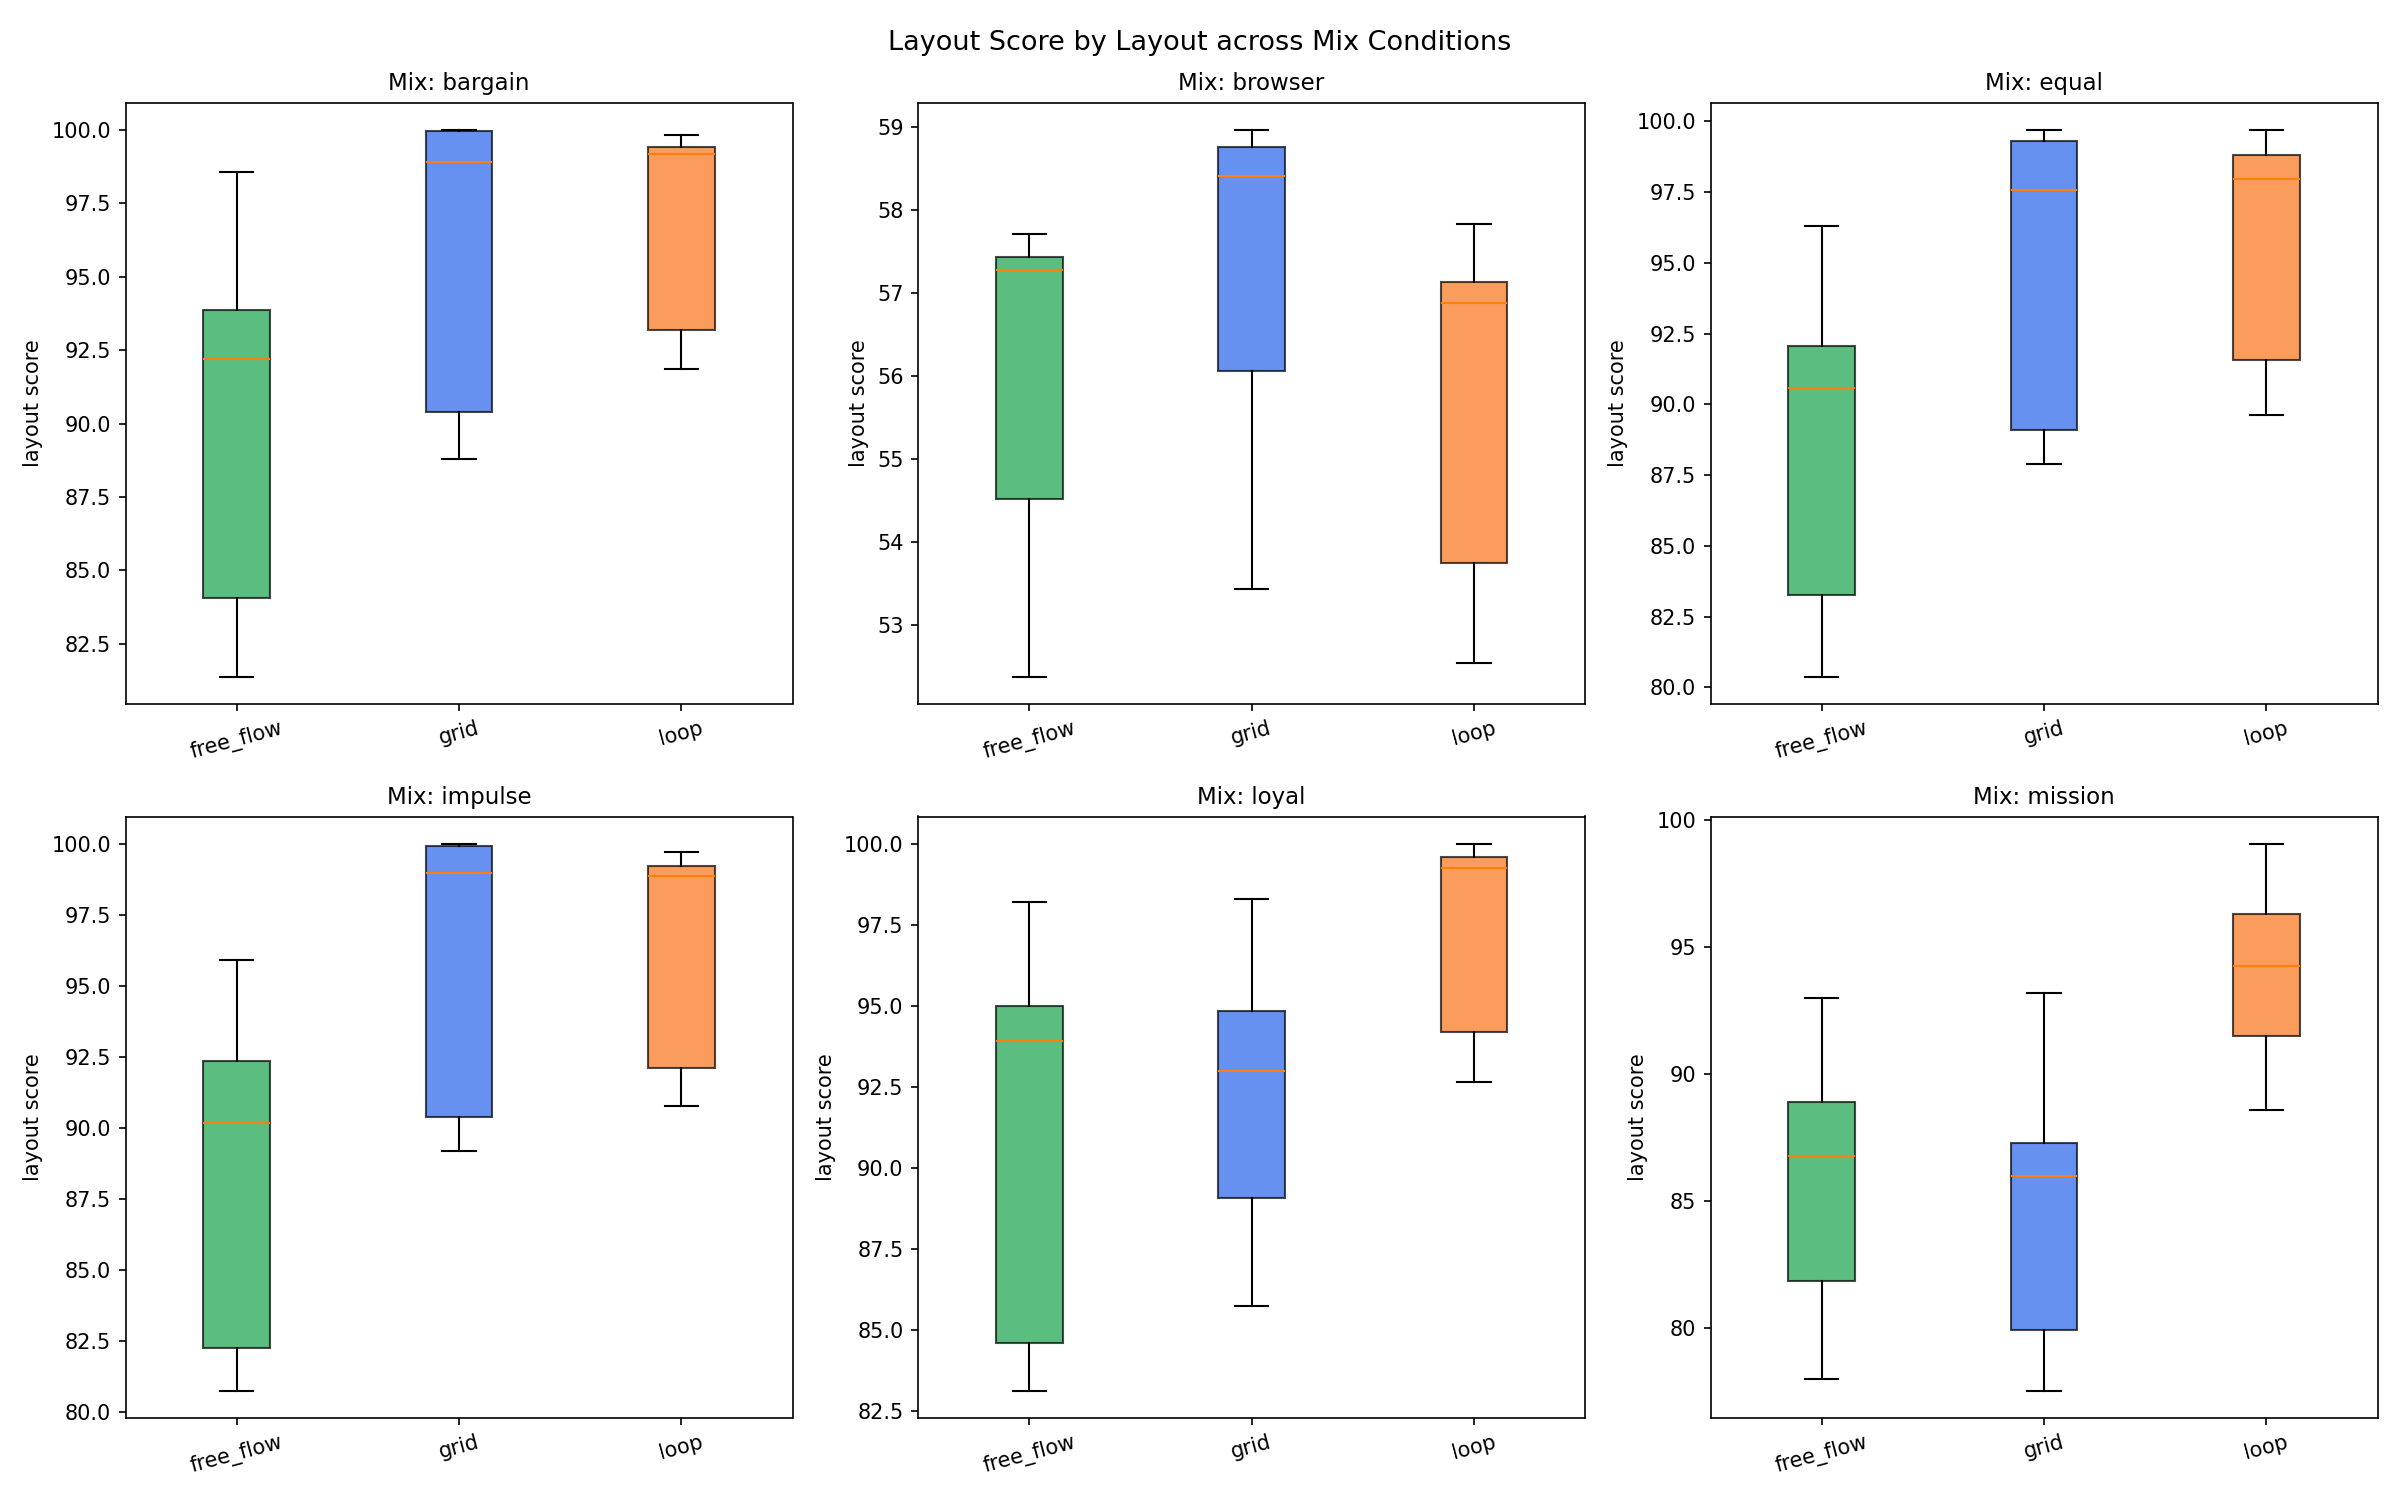
\includegraphics[width=0.82\columnwidth]{boxplot_layout_score.png}
\caption{Overall layout score by density, layout, and shopper mix. The line chart shows density trends, while the boxplot summarizes run-level score distributions.}
\Description{Layout-score line chart and boxplot for grid, loop, and free-flow layouts across shopper mixes.}
\label{fig:layout-score}
\end{figure}

Figure~\ref{fig:layout-score} shows that loop is the best balanced layout for most list-carrying shopper populations because it combines strong planned completion with high unplanned purchasing. Grid leads browsers because browsers receive no planned-completion benefit from loop, so the faster and less frustrating grid layout becomes more favorable. The mixed score pattern is consistent with servicescape and atmospherics research: the same physical environment can support some customer goals while hindering others \citep{mari2013,spence2014}.

\subsection{Density-Stratified Layout Score}

The density-stratified layout-score boxplots isolate how each shopper mix responds to layout at 50, 150, and 400 shoppers. This is important because the two-way ANOVA summaries showed that layout effects interact with density. In practical terms, a layout that performs adequately when the store is lightly occupied may perform very differently when shopper density rises.

\begin{figure}[t]
\centering
\begin{minipage}{0.48\columnwidth}
    \centering
    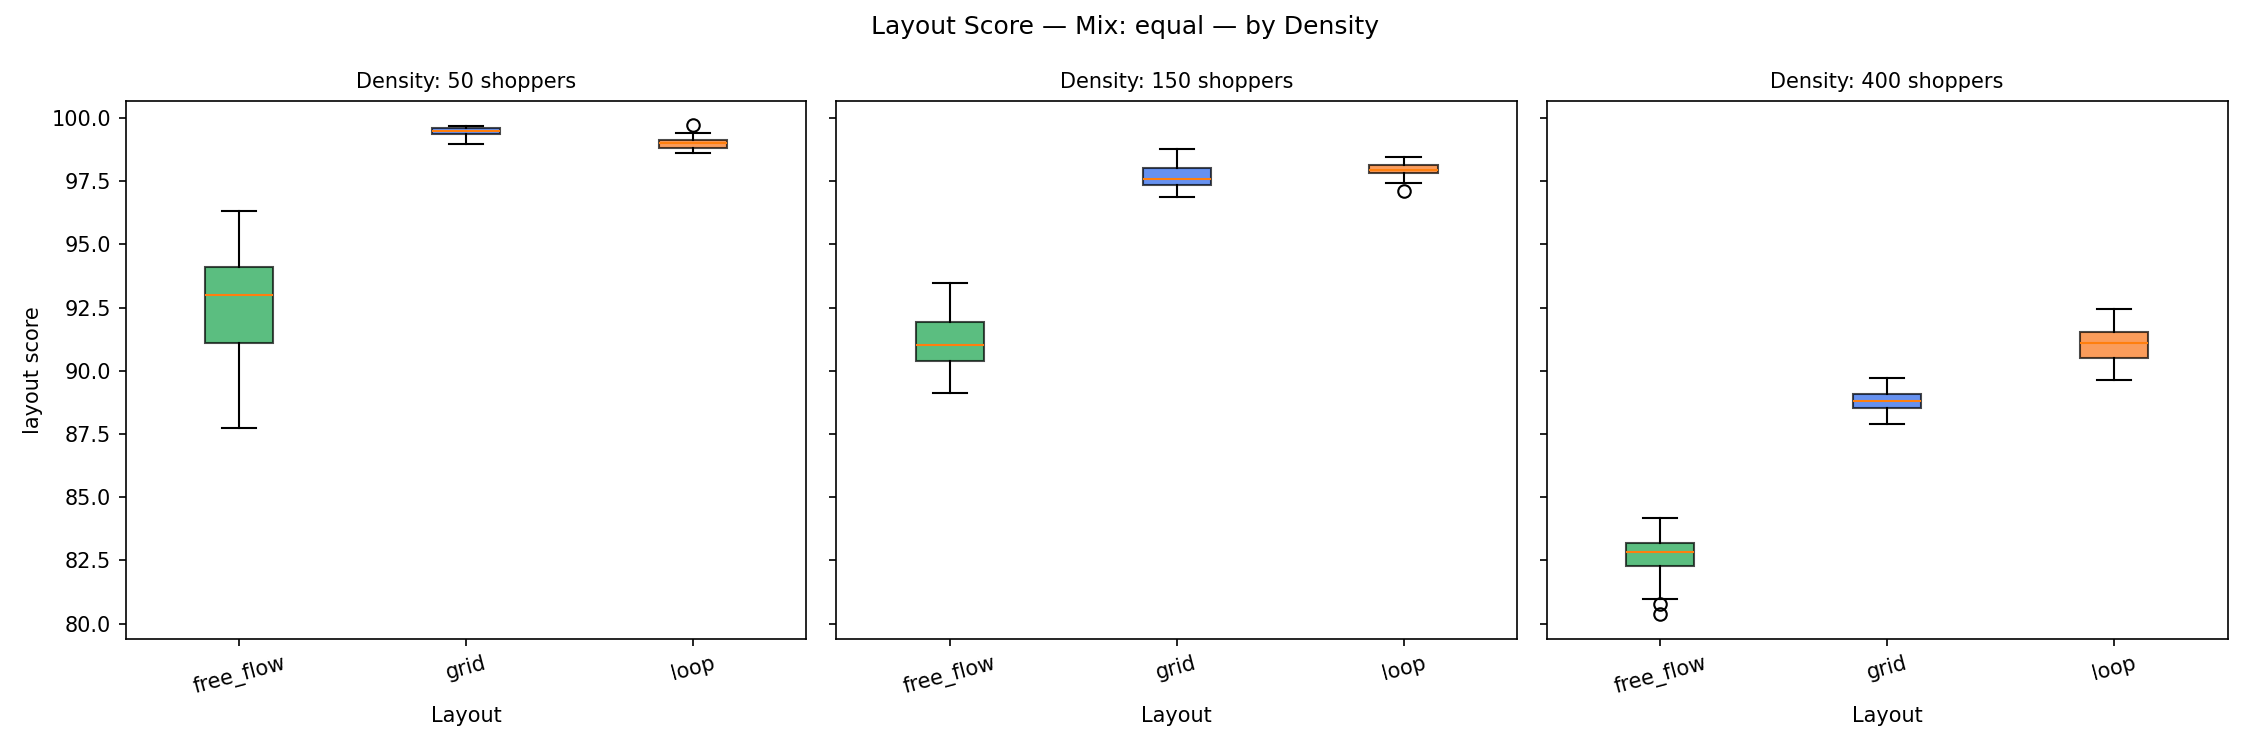
\includegraphics[width=\linewidth]{boxplot_density_layout_score_equal.png}
\end{minipage}
\hfill
\begin{minipage}{0.48\columnwidth}
    \centering
    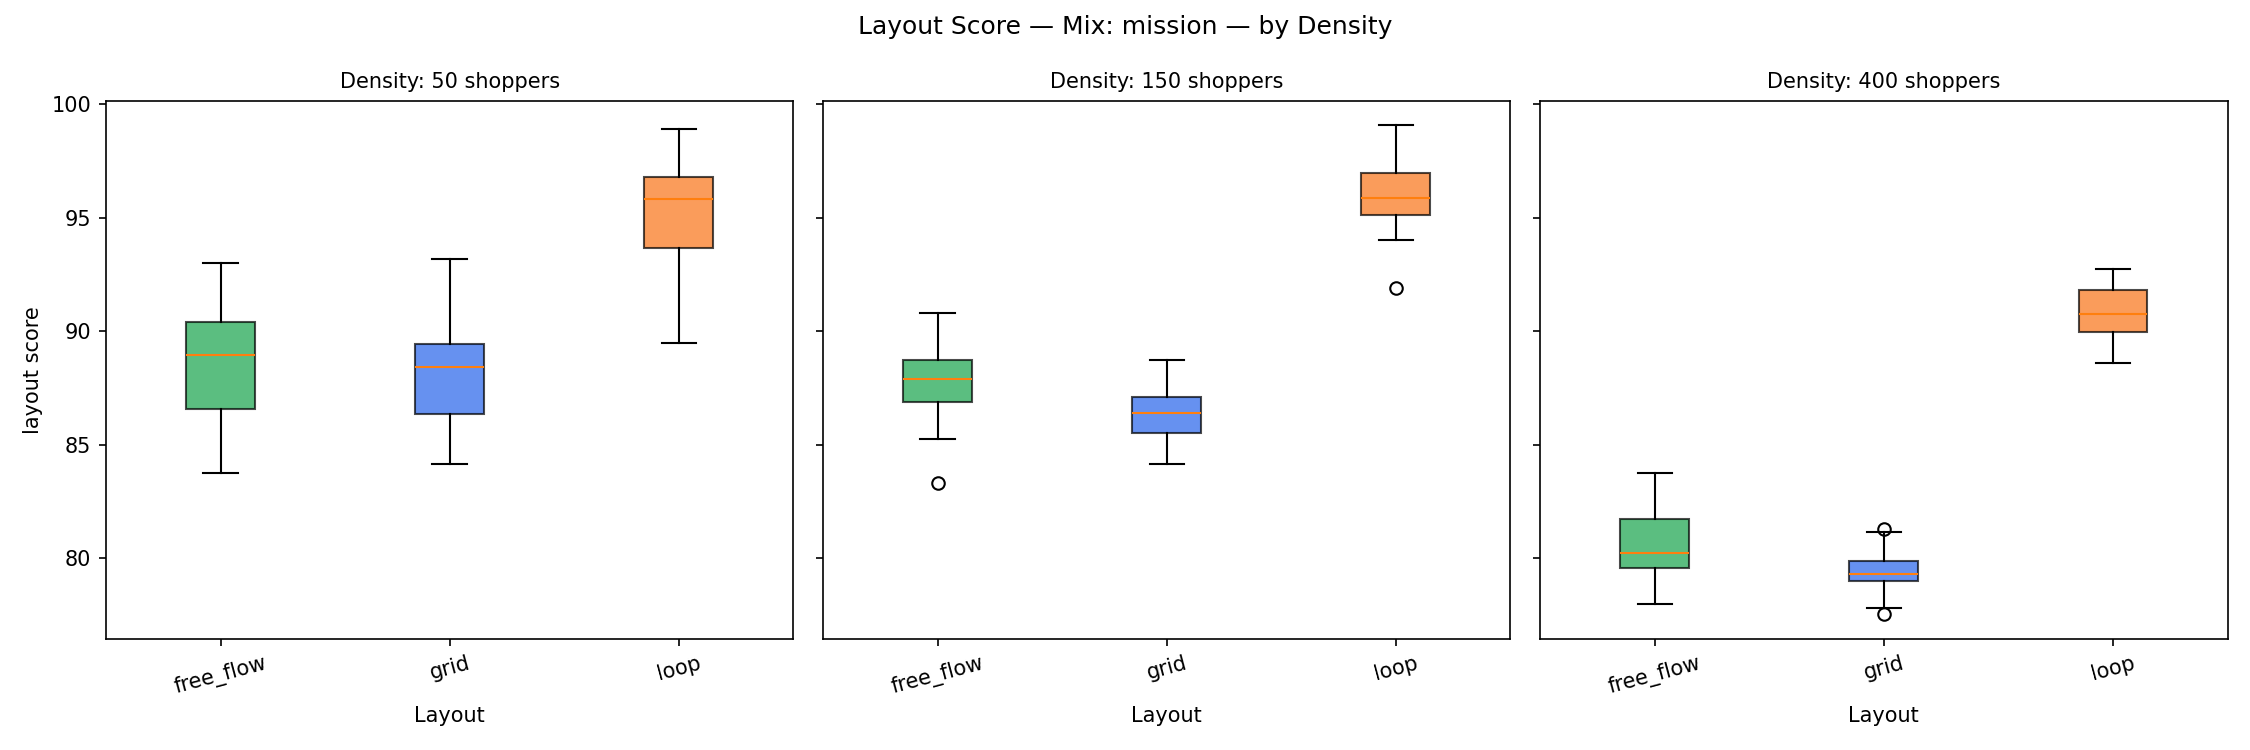
\includegraphics[width=\linewidth]{boxplot_density_layout_score_mission.png}
\end{minipage}
\vspace{0.08in}
\begin{minipage}{0.48\columnwidth}
    \centering
    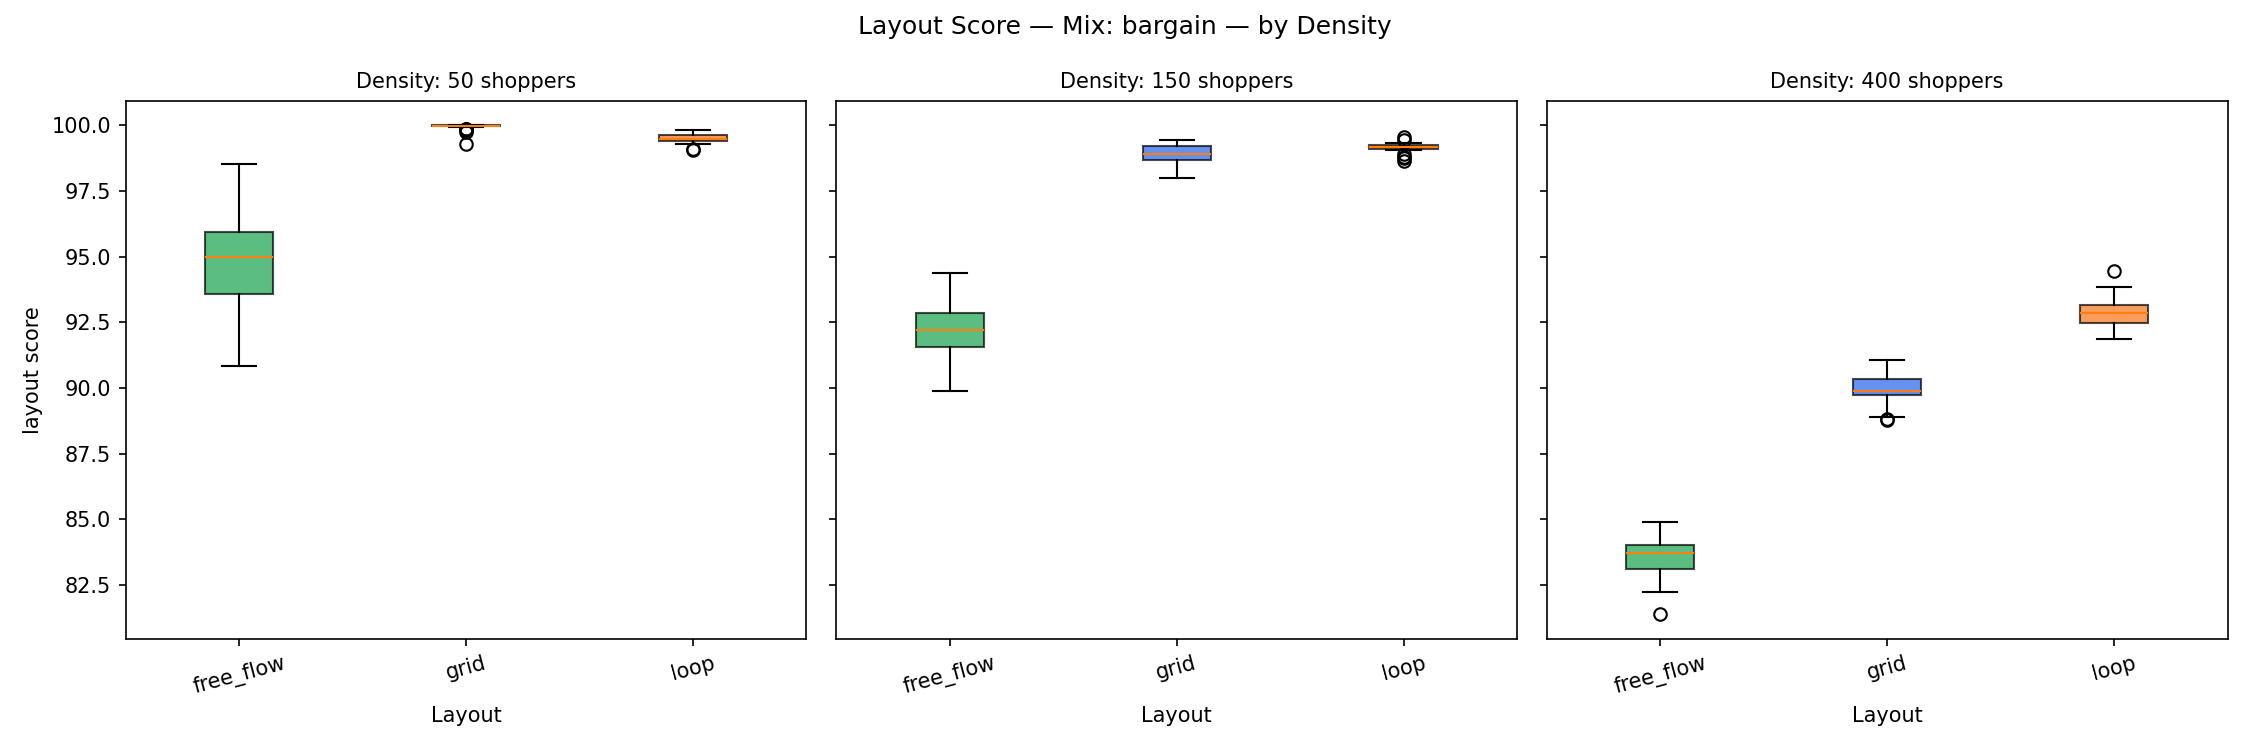
\includegraphics[width=\linewidth]{boxplot_density_layout_score_bargain.png}
\end{minipage}
\hfill
\begin{minipage}{0.48\columnwidth}
    \centering
    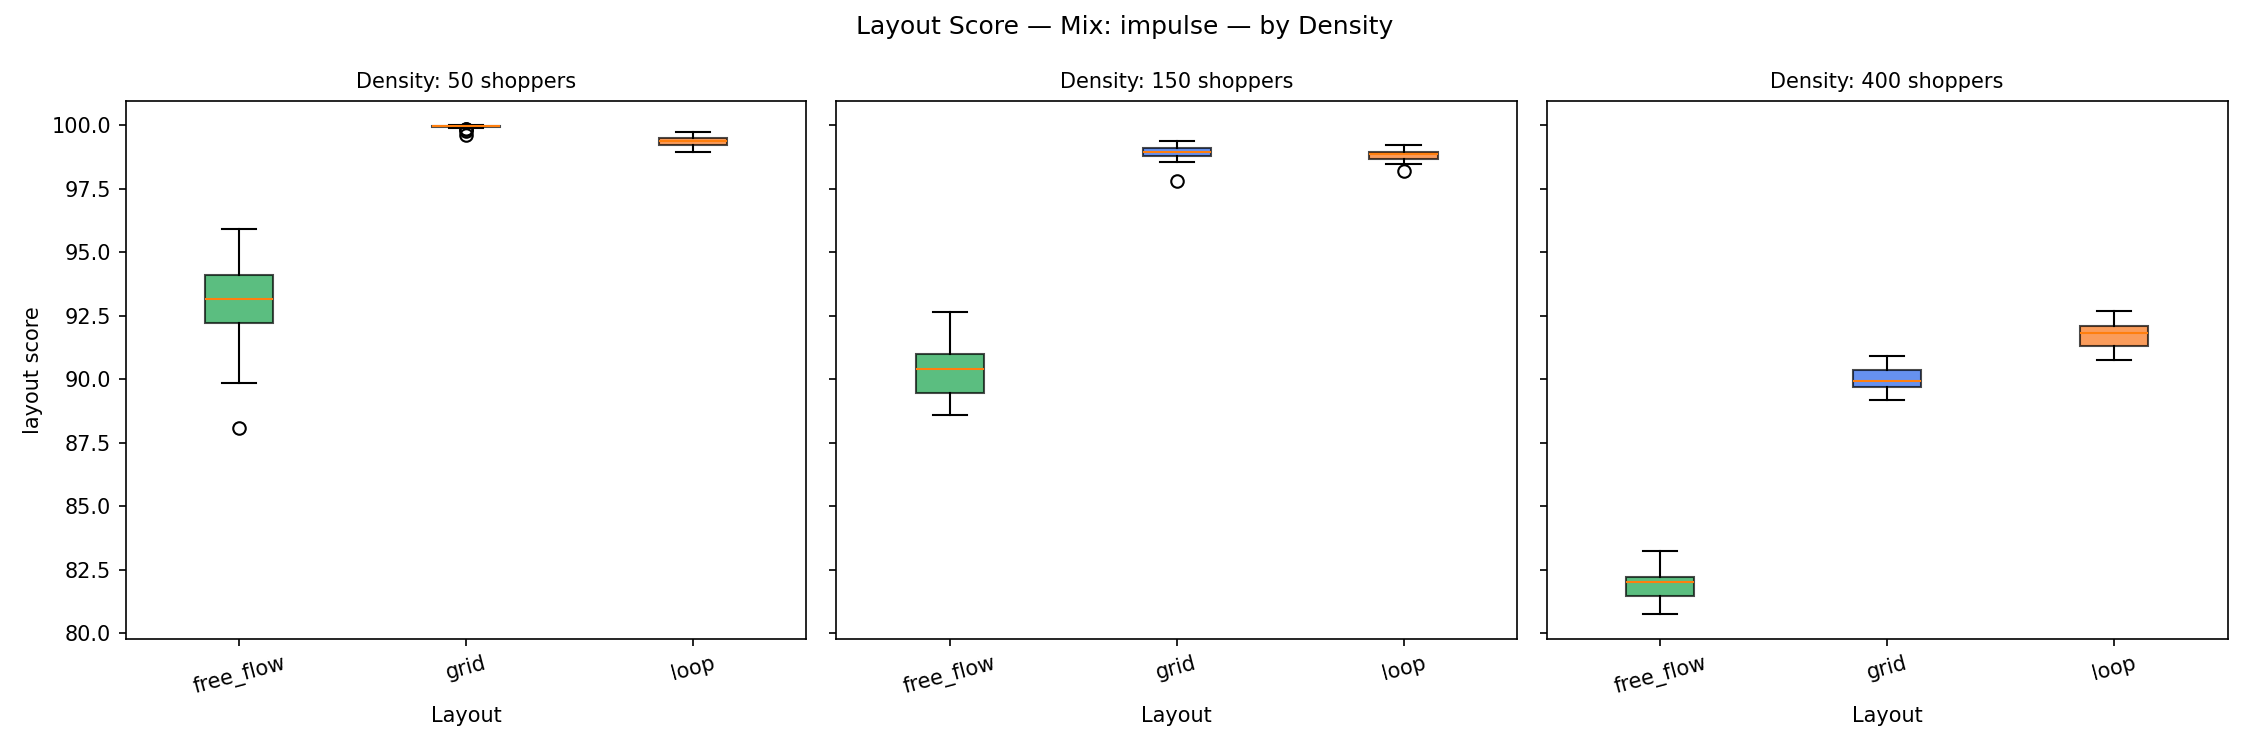
\includegraphics[width=\linewidth]{boxplot_density_layout_score_impulse.png}
\end{minipage}
\vspace{0.08in}
\begin{minipage}{0.48\columnwidth}
    \centering
    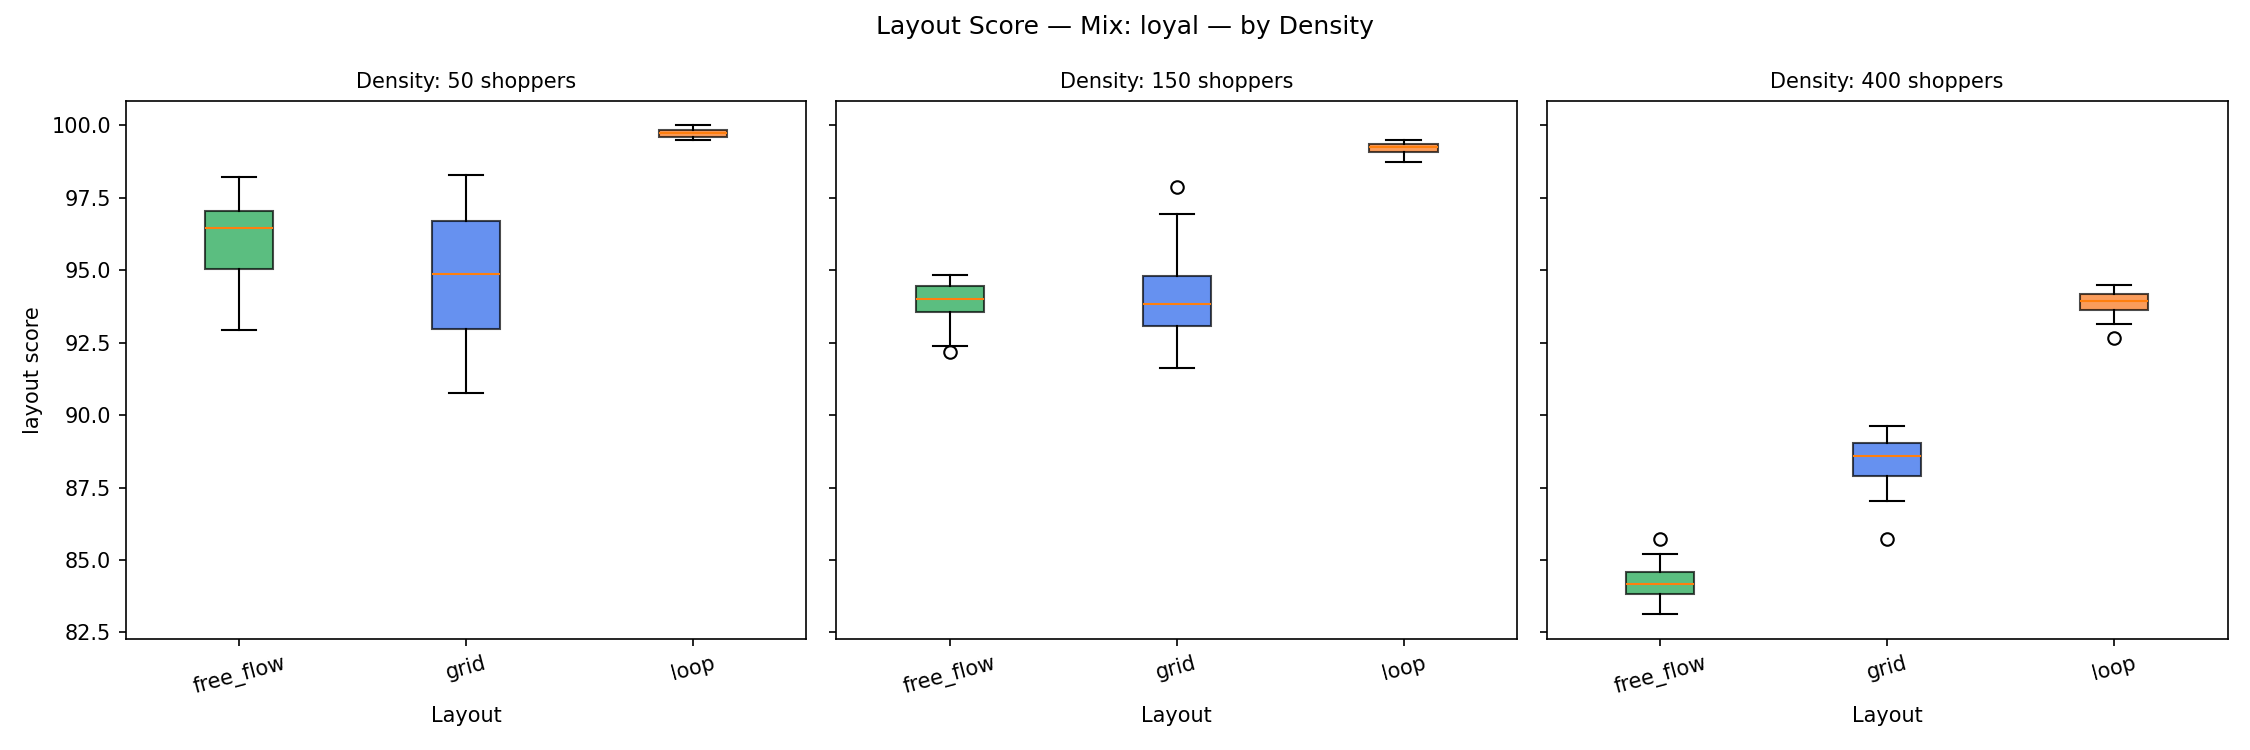
\includegraphics[width=\linewidth]{boxplot_density_layout_score_loyal.png}
\end{minipage}
\hfill
\begin{minipage}{0.48\columnwidth}
    \centering
    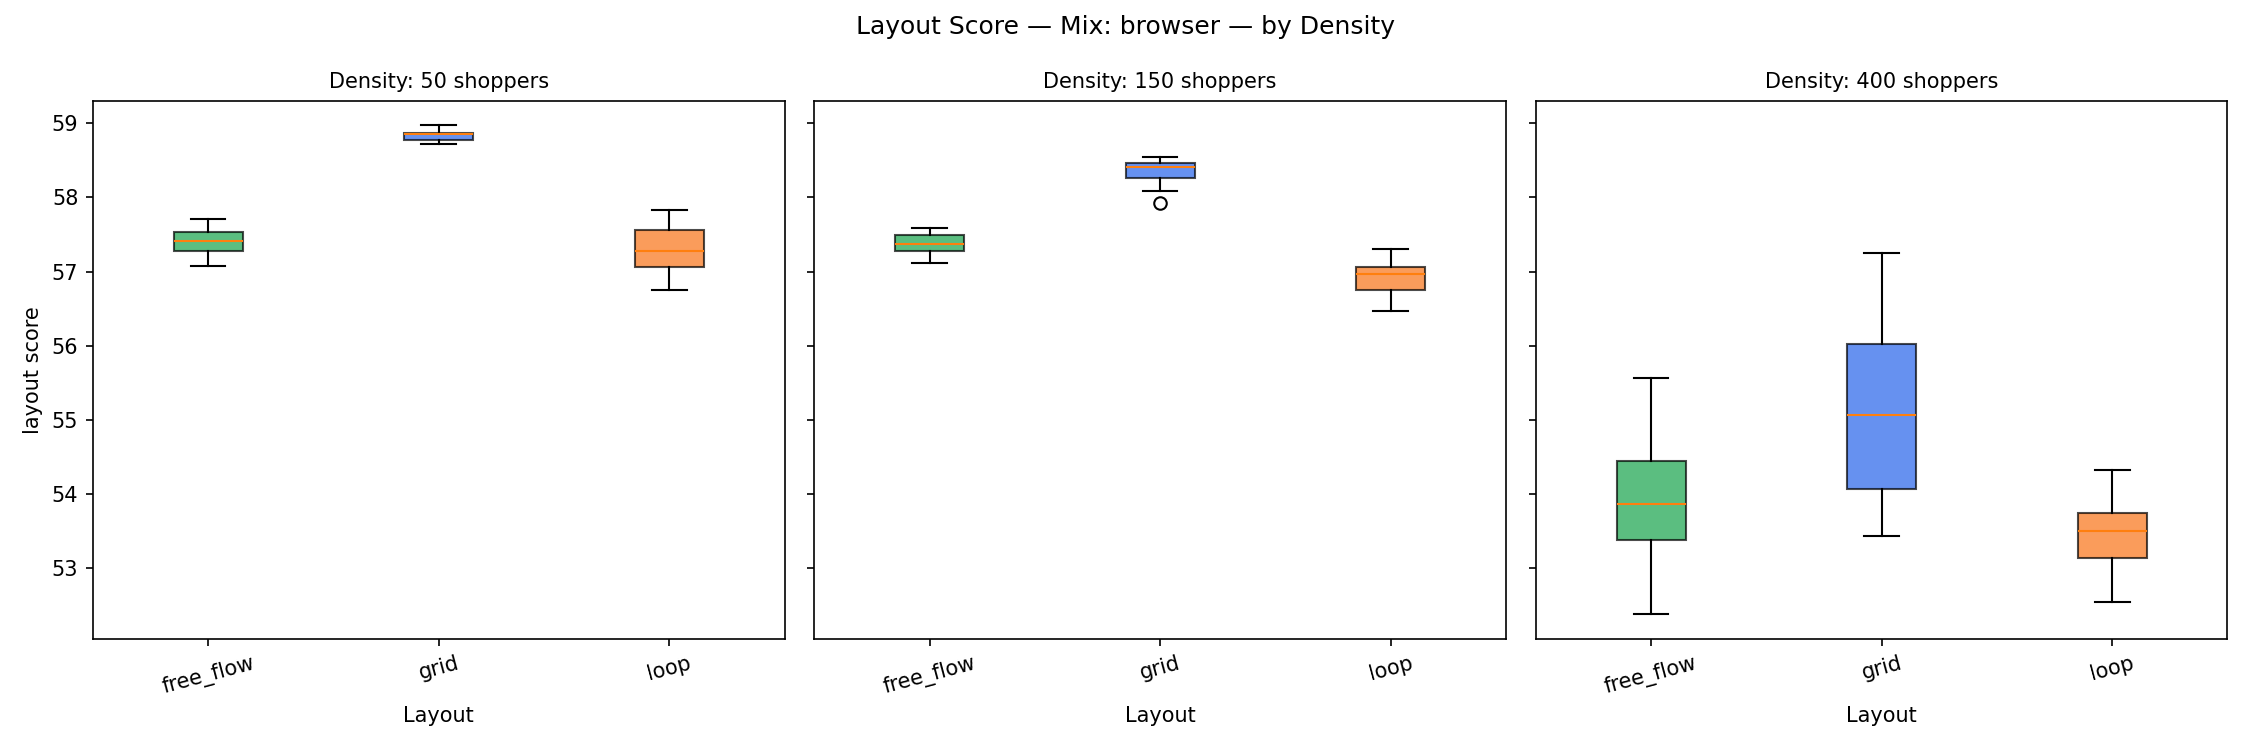
\includegraphics[width=\linewidth]{boxplot_density_layout_score_browser.png}
\end{minipage}
\caption{Density-stratified layout-score boxplots for all six shopper mixes. Each panel isolates one shopper mix and compares layout-score distributions across the three density levels.}
\Description{Six density-stratified layout-score boxplots for equal, mission-driven, bargain-hunter, impulse-buyer, loyal-shopper, and browser mixes.}
\label{fig:density-layout-score}
\end{figure}

Figure~\ref{fig:density-layout-score} explains why the paper emphasizes the 400-shopper scenario. At 50 and 150 shoppers, the layouts are often closer because most agents can move and complete trips without severe competition for space. At 400 shoppers, the distributions separate more clearly: loop leads most list-carrying mixes, while grid remains strongest for browsers. This supports density-aware layout evaluation \citep{pantano2021} and crowding research showing that store density affects customer outcomes \citep{blut2020,aydinli2021}.

\subsection{Overall Layout Effect Sizes}

The overall effect-size plot summarizes how strongly layout separates each outcome. This is different from the line charts and boxplots because it focuses on magnitude of statistical difference rather than only central tendency or visual distribution. Large effects indicate that the layout variable has a meaningful impact on the outcome being measured.

\begin{figure}[t]
\centering
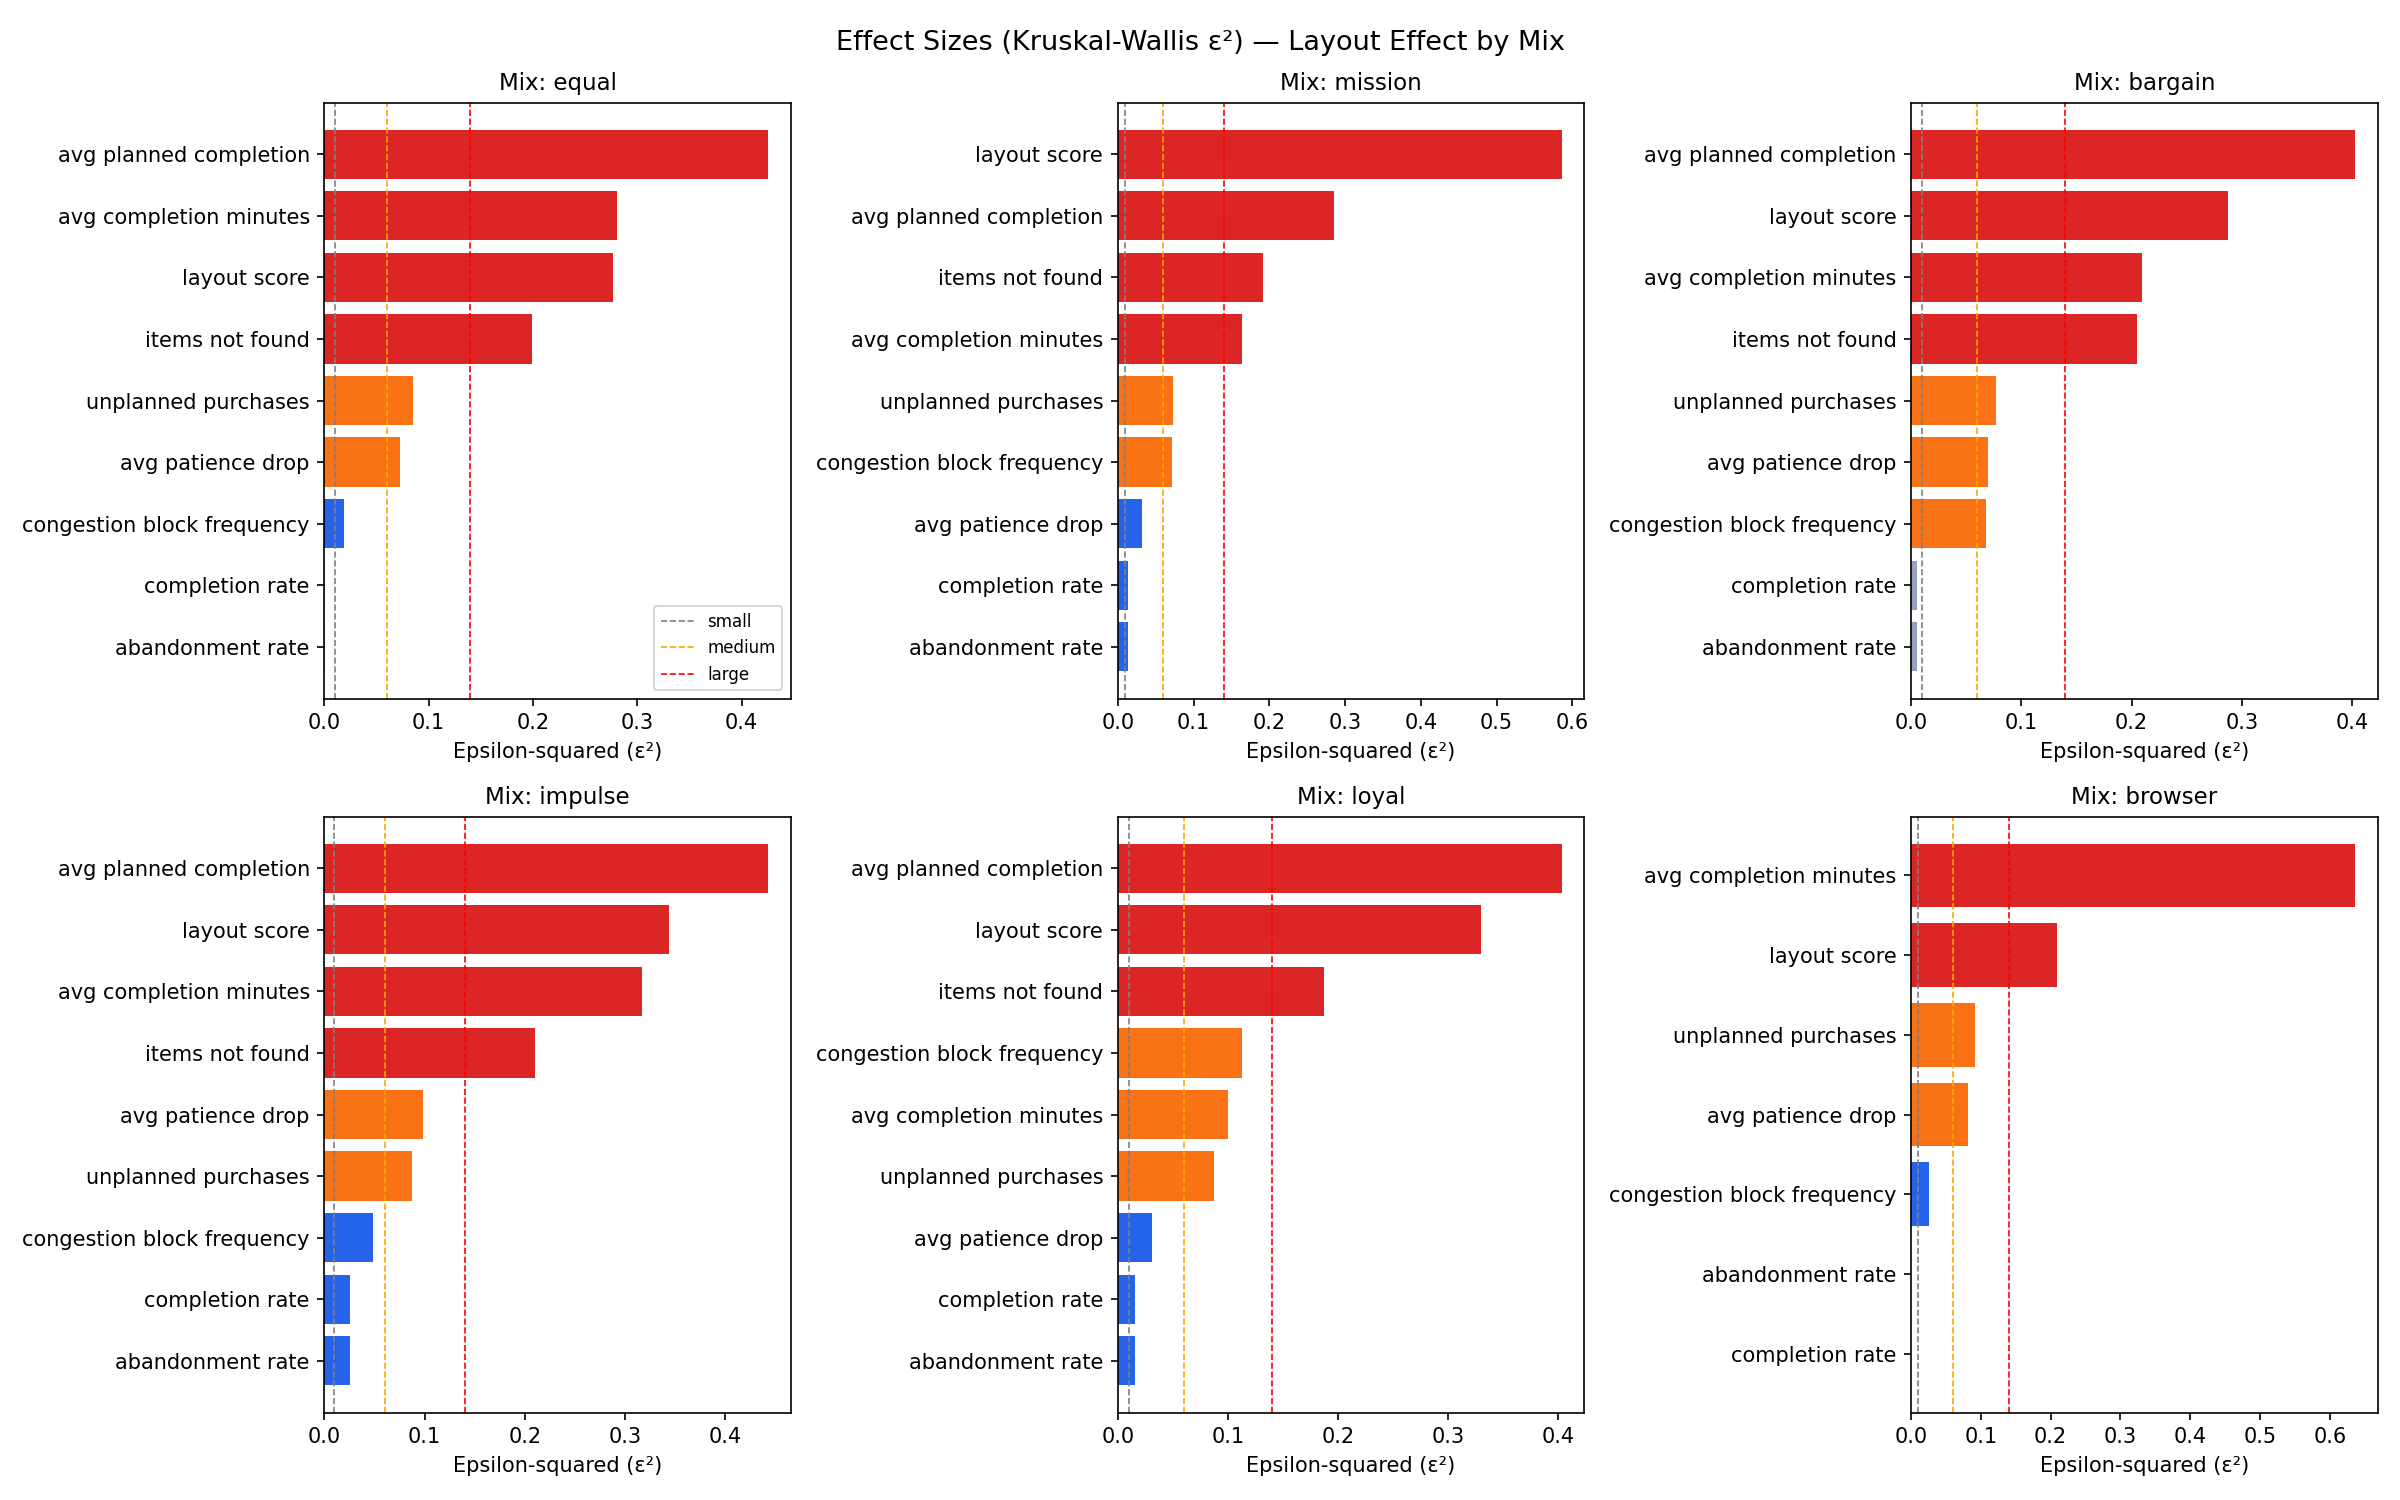
\includegraphics[width=\columnwidth]{effect_sizes.png}
\caption{Overall layout effect sizes across final simulation outcomes. Larger values indicate stronger layout effects for the corresponding metric.}
\Description{Effect-size plot summarizing the magnitude of layout effects across simulation outcomes.}
\label{fig:overall-effect-sizes}
\end{figure}

Figure~\ref{fig:overall-effect-sizes} shows that the strongest layout effects occur for outcomes directly tied to route structure and product discovery. This supports the claim that layout is not a superficial design choice; it changes the behavioral conditions under which shoppers search, move, complete lists, encounter products, and decide whether to finish the trip. The interpretation is consistent with research treating store layout and atmospherics as behavior-shaping retail conditions \citep{mari2013,spence2014,hwangbo2017}.

\subsection{Density-Stratified Effect Sizes}

The density-stratified effect-size heatmap separates layout effect magnitude by shopper mix, density level, and outcome. This diagnostic is useful because some layout effects appear small when averaged across all densities but become stronger under high-density conditions.

\begin{figure}[t]
\centering
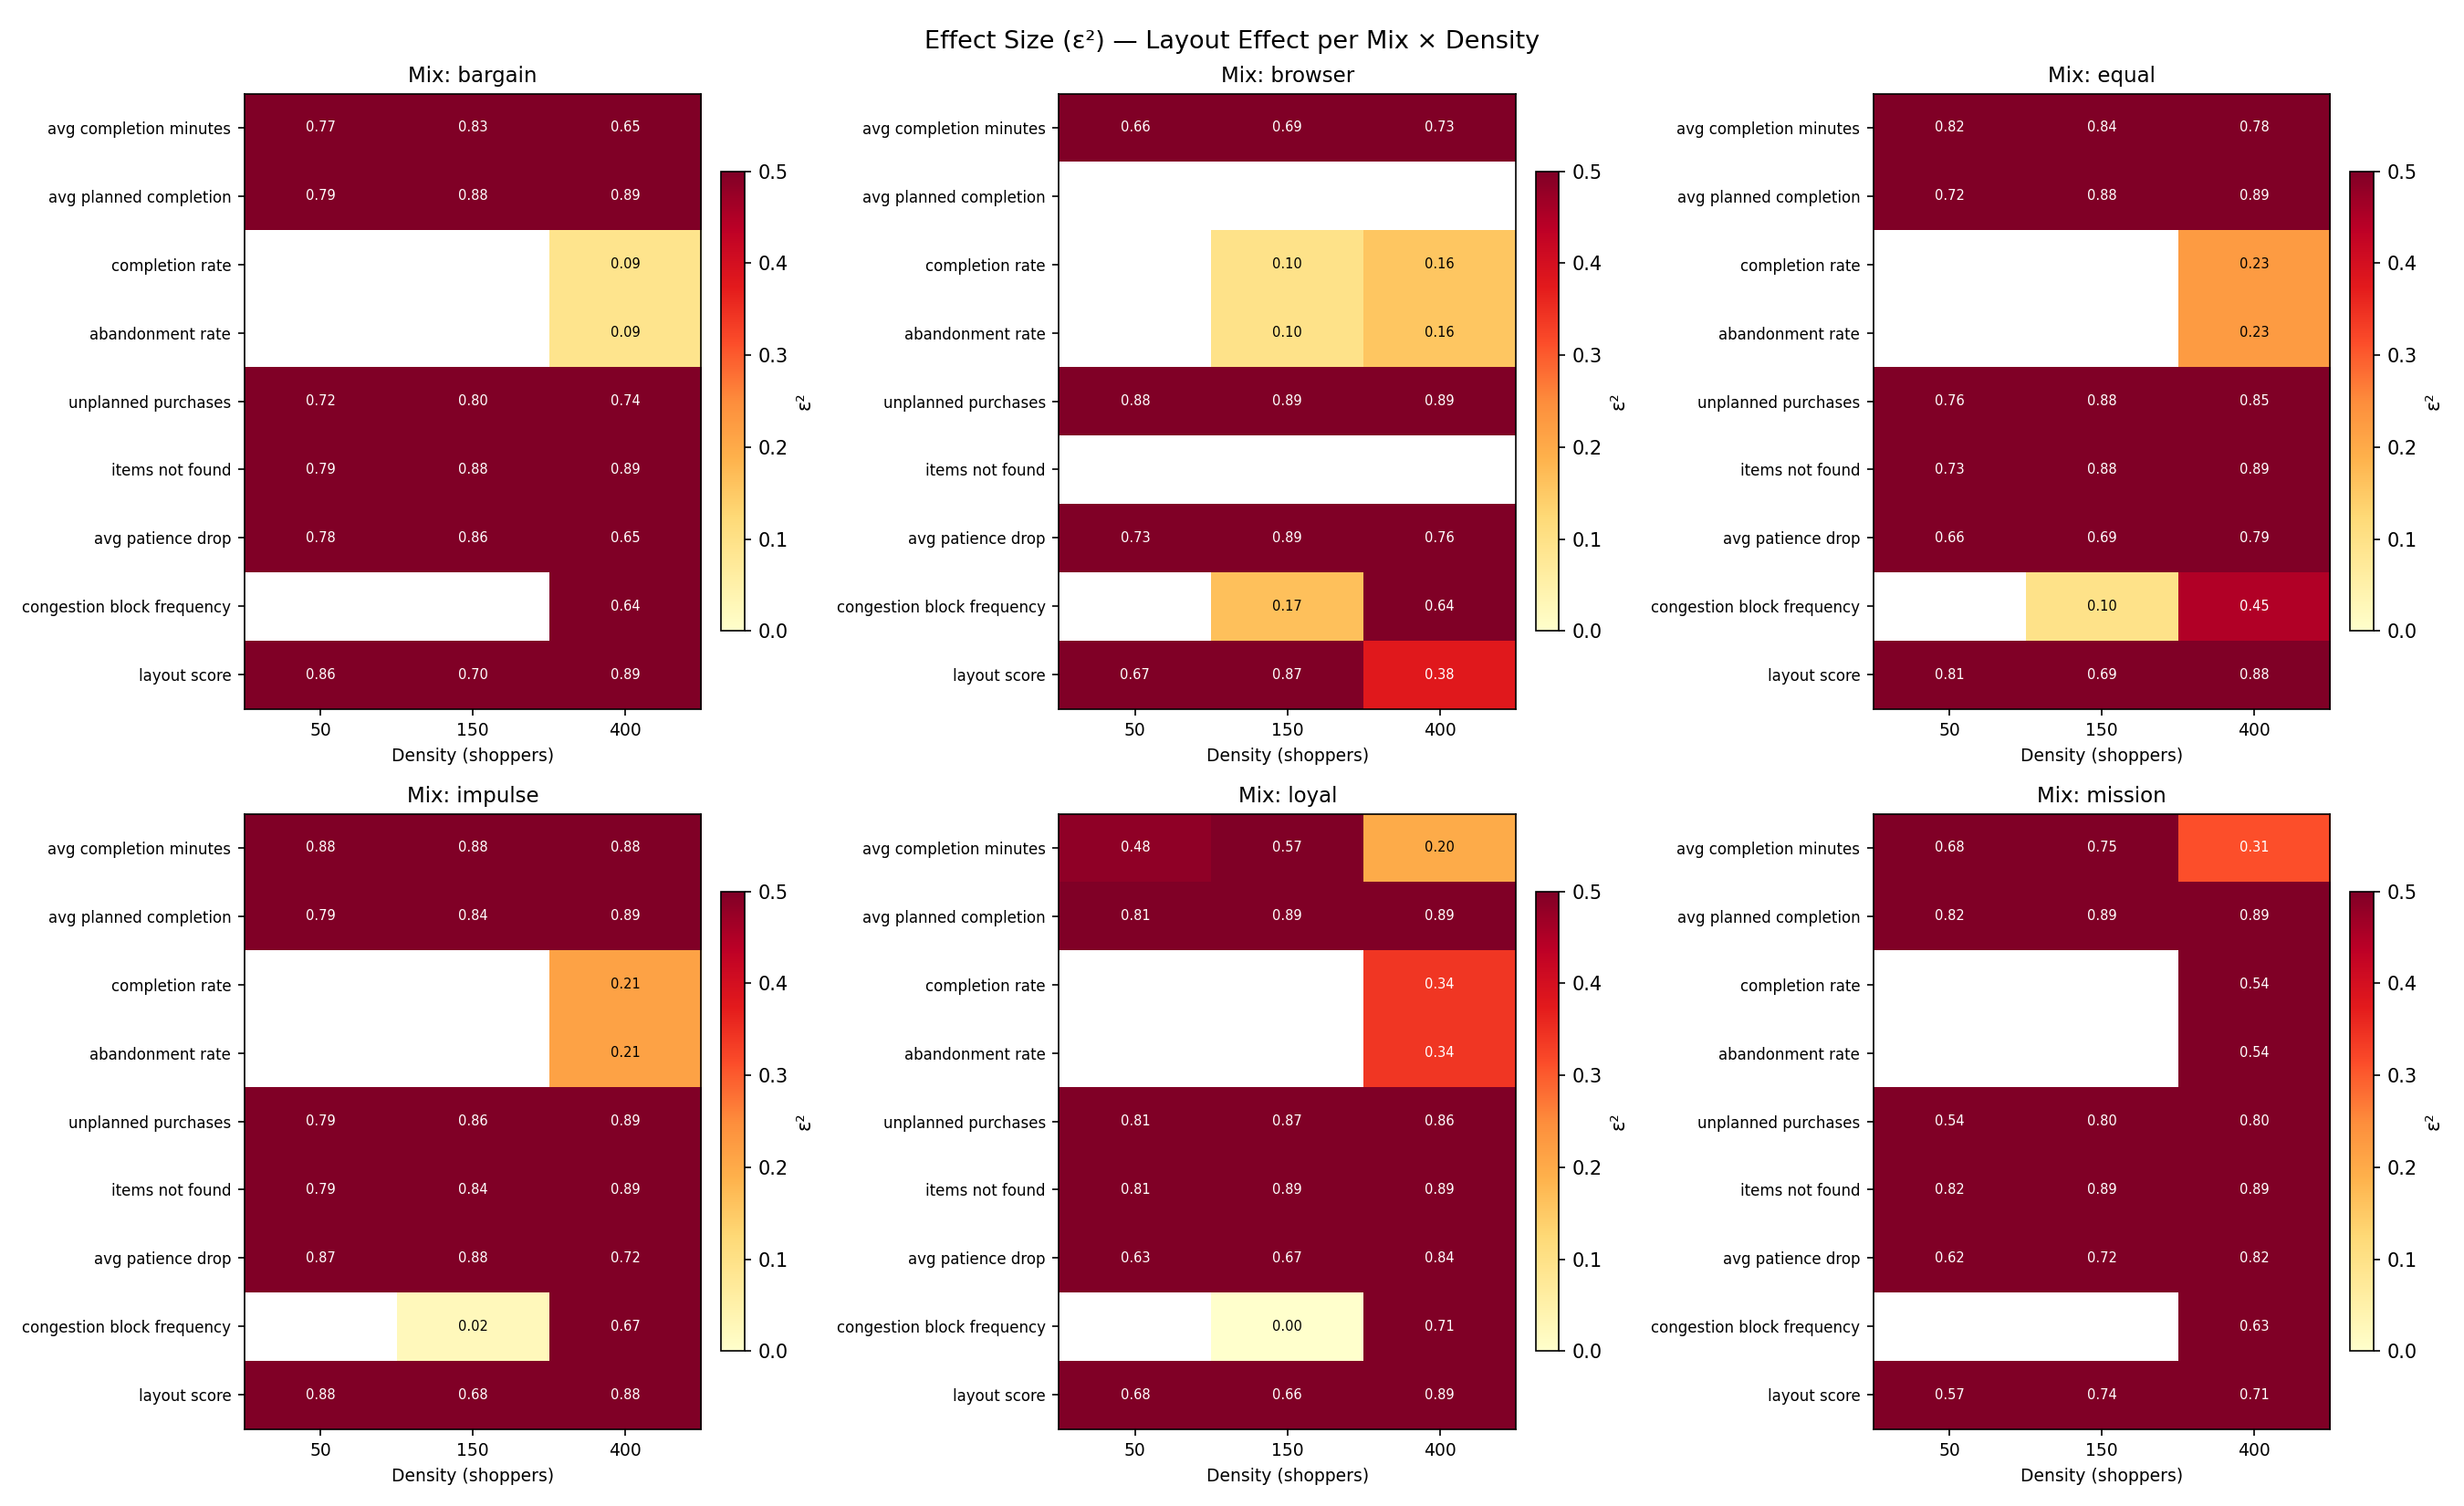
\includegraphics[width=\columnwidth]{effect_size_heatmap_by_density.png}
\caption{Density-stratified effect-size heatmap. Stronger color intensity indicates stronger layout effects within a shopper mix, density level, and outcome.}
\Description{Heatmap of effect sizes for layout effects by density, shopper mix, and outcome.}
\label{fig:density-effect-sizes}
\end{figure}

Figure~\ref{fig:density-effect-sizes} shows that layout effects concentrate in planned completion, items not found, completion time, and layout score, especially at higher density. This strengthens the main result because it shows that layout effects are not uniform across all scenarios. They become more important when traffic pressure increases, which is consistent with agent-based store-density research \citep{pantano2021} and retail-crowding evidence \citep{blut2020,aydinli2021}.

\subsection{High-Density Layout Leaders}

Table~\ref{tab:high-density-results} summarizes the high-density leaders for the major outcome categories. The table is useful because it makes the layout trade-off explicit: grid leads efficiency, loop leads list completion and unplanned purchasing, and the highest composite score depends on whether the shopper mix is list-carrying or browser-dominant.

\begin{table*}[t]
\caption{High-density (400 shoppers) layout leaders from final simulation outputs}
\label{tab:high-density-results}
\small
\begin{tabular}{@{}lllll@{}}
\toprule
\textbf{Mix} & \textbf{Fastest completion} & \textbf{Best list completion} & \textbf{Most unplanned purchases} & \textbf{Highest score} \\
\midrule
Equal & Grid 211.2 & Loop 0.886 & Loop 1,725.6 & Loop 91.1 \\
Mission-driven & Loop 201.0 & Loop 0.894 & Loop 401.6 & Loop 90.8 \\
Bargain-hunter & Grid 209.9 & Loop 0.901 & Loop 1,430.4 & Loop 92.9 \\
Impulse-buyer & Grid 202.8 & Loop 0.889 & Loop 3,615.0 & Loop 91.7 \\
Loyal-shopper & Grid 206.4 & Loop 0.938 & Loop 725.6 & Loop 93.9 \\
Browser & Grid 245.2 & N/A & Loop 2,243.2 & Grid 55.1 \\
\bottomrule
\end{tabular}
\end{table*}

The high-density summary confirms that no single layout dominates every metric. Grid is the strongest efficiency layout, loop is the strongest exposure and list-coverage layout, and free-flow is not the best high-density grocery layout in the final experiments. This conditional pattern is important for the Discussion because it means that the recommended layout depends on the store objective rather than on a universal ranking.

\clearpage

\section{Discussion}

The final six-mix result set rejects the null hypothesis for the primary outcomes. Layout changed movement efficiency, planned-list completion, unplanned purchases, patience loss, congestion, abandonment, and the composite layout score. This conclusion is stronger than a visual comparison of averages because it is supported by nonparametric layout tests, density-stratified tests, chi-square tests, correlation analysis, traffic heatmaps, and the metric-specific visual diagnostics in Figures~\ref{fig:grid-traffic-heatmap}--\ref{fig:density-effect-sizes}. It is also consistent with newer retail research showing that physical store environments, atmospherics, customer movement, and consumer density can shape shopping behavior and layout performance \citep{mari2013,spence2014,hwangbo2017,pantano2021}.

The grid layout should be interpreted as the efficiency-focused layout. It was fastest in five of the six high-density mixes and produced the lowest patience drop in all six. This does not mean grid is always the highest-value layout, but it does mean grid is the safest choice when the store objective is fast completion, low friction, and lower abandonment risk. The finding is supported by indoor-positioning research showing that in-store movement patterns can be connected to sales and layout optimization \citep{hwangbo2017}; if a layout creates more predictable paths, it can reduce the search and congestion costs produced by many simultaneous shoppers. This also fits agent-based store-density work arguing that layout decisions should be tested under crowding rather than evaluated only in isolation \citep{pantano2021}.

The loop layout should be interpreted as a layout for exposure and coverage. It produced the highest unplanned-purchase count in every high-density mix and gave the best planned-list completion for every list-carrying mix. This two-sided result is important: loop did not only push impulse purchases; it also helped shoppers encounter planned product zones. The unplanned-purchase pattern is strongly supported by Hui et al. \citeyearpar{hui2013}, who found that in-store travel distance can increase unplanned spending. It is also supported by impulse-buying research showing that store stimuli, product characteristics, promotions, and shopper impulse tendency influence unplanned purchases \citep{bellini2017,kacen2012,stilley2010}. The planned-completion pattern is supported by grocery product-arrangement and store-layout research showing that product grouping, shelf organization, aisle space, and product availability affect how shoppers find items \citep{seva2019,andrada2020}.

The free-flow layout is the weakest grocery layout in the final experiments, especially at high density. It encouraged exploration and often generated more unplanned purchases than grid, but it also produced the weakest list completion, the most items not found, and higher patience loss. This suggests that exploration without enough route structure is risky for grocery shopping, where customers often expect to locate staple categories efficiently. The result is consistent with grocery product-arrangement research showing that shoppers expect meaningful relationships among categories \citep{seva2019}, and with newer servicescape research arguing that physical environments influence whether customers can accomplish their goals \citep{mari2013,spence2014}. In this simulation, free-flow did not provide enough systematic coverage to compensate for its search cost.

Shopper mix changes which layout is most defensible. Impulse buyers and bargain hunters reward exposure because additional product contact can become additional purchasing, which is consistent with impulse-buying, travel-distance, and merchandising research \citep{hui2013,bellini2017,kacen2012}. Loyal shoppers reward loop because familiarity lowers the cost of guided circulation while preserving high list completion; this matches product-arrangement research showing that expected product relationships can guide grocery search \citep{seva2019}. Mission-driven shoppers remain efficient in both grid and loop, but loop improves list coverage. Browsers create the clearest warning: they generate many unplanned purchases in loop, but the same exposure increases time, patience loss, and abandonment. Their result supports newer crowding studies showing that density can reduce perceived control, affect basket composition, and change behavior near shelves \citep{blut2020,aydinli2021,luck2015}.

The practical implication is that layout choice should be tied to the store's dominant problem. If the store suffers from crowding, long trips, or high checkout abandonment, grid is the most defensible option. If the store wants stronger product exposure while still helping list-carrying shoppers pass more categories, loop is the best balanced option. If the store is a specialty or browsing-oriented shop, free-flow may be useful, but the final results do not support it as the best choice for a high-density grocery environment. In short, the simulation supports a conditional recommendation rather than a single universal answer: grid for efficiency and congestion control, loop for exposure and guided coverage, and free-flow only when exploration is more important than reliable grocery completion.

\section{Limitations}

The model is a simplified representation of grocery shopping. Product arrangement is predetermined, so the experiment changes layout type but does not optimize item placement inside each layout. Travel time may also be unrealistic in some cases because every step represents a simplified one-tile movement rather than a calibrated human walking speed. In addition, the number of shelf cells differs across layouts, which may create a correlation between layout structure and product availability. This is defensible as a fixed-footprint modeling choice, but future work should separate layout geometry from assortment size.

The final result set covers six shopper mixes, which gives broader support than the earlier presentation runs. However, each mix is still a scenario design rather than a direct sample from an observed grocery population. Future work should estimate shopper-mix proportions from real transaction data, entrance counts, or in-store tracking so that simulated traffic more closely matches a specific store.

The numerical parameters for patience thresholds, impulse multipliers, exposure radius, tile capacity, and layout-score weights are calibrated scenario settings. The literature supports the behavioral mechanisms, but it does not prove one exact threshold for every store. Future experiments should run sensitivity analysis on these parameters and test whether the same layout ranking holds under alternative assumptions.

\section{Conclusion}

The agent-based simulation demonstrates that grocery store layout has a meaningful effect on consumer movement, shopping efficiency, and purchasing behavior across the six final shopper-mix experiments. The null hypothesis is rejected: layout significantly changed completion time, planned-list completion, unplanned purchases, missed items, patience loss, congestion, abandonment, and layout score. This conclusion is consistent with 2010-and-newer retail-layout, servicescape, and store-atmosphere research showing that the physical retail environment influences shopper behavior \citep{mari2013,spence2014,hwangbo2017,ozgormus2020,pantano2021}.

The strongest finding is the trade-off between efficiency and exposure. Grid protected the shopping experience by reducing completion time and patience loss, which makes it the best layout when the priority is fast, reliable shopping and congestion control. Loop produced the strongest unplanned-purchase outcomes and the best high-density planned-list completion for list-carrying shoppers, making it the best balanced layout when the store wants both exposure and product-zone coverage. These findings are supported by research on product arrangement and grocery search \citep{seva2019,andrada2020}, in-store travel distance and unplanned spending \citep{hui2013}, impulse buying \citep{bellini2017,kacen2012,stilley2010}, and retail crowding \citep{blut2020,aydinli2021}.

Free-flow encouraged exploration but performed poorly under high density because it increased missed items and patience loss. Therefore, the final recommendation is conditional: use grid when the store's main problem is speed, crowding, or abandonment; use loop when the goal is stronger exposure and guided category coverage; and use free-flow only when browsing experience is more important than reliable grocery completion. The right layout depends on who is shopping, how crowded the store is, and whether the retailer prioritizes operational efficiency, revenue-oriented exposure, or a weighted balance of both.

\section*{Acknowledgments}

The authors thank PAULA E. MAYOL for her guidance, instruction, and feedback throughout CMSC 176. This paper was prepared from the project's Mesa implementation, final simulation CSV outputs, \texttt{stats\_analysis.py}, research notes, and final presentation slides.

\begin{thebibliography}{99}

\bibitem[Andrada et~al.(2020)]{andrada2020}
Andrada, M. F., Prudenciano, H. L., \& Reyes, J. B. (2020). Layout design model for independent grocery stores in the Philippines. In \emph{Proceedings of the International Conference on Industrial Engineering and Operations Management} (pp. 1719--1729). IEOM Society International. \url{https://www.ieomsociety.org/ieom2020/papers/272.pdf}

\bibitem[Angeles-Agdeppa et~al.(2019)]{angeles2019}
Angeles-Agdeppa, I., Sun, Y., Denney, L., Tanda, K. V., Octavio, R. A. D., Carriquiry, A., \& Capanzana, M. V. (2019). Food sources, energy and nutrient intakes of adults: 2013 Philippines National Nutrition Survey. \emph{Nutrition Journal, 18}, Article 59. \url{https://doi.org/10.1186/s12937-019-0481-z}

\bibitem[Aydinli et~al.(2021)]{aydinli2021}
Aydinli, A., Lamey, L., Millet, K., ter Braak, A., \& Vuegen, M. (2021). How do customers alter their basket composition when they perceive the retail store to be crowded? An empirical study. \emph{Journal of Retailing, 97}(2), 207--216. \url{https://doi.org/10.1016/j.jretai.2020.05.004}

\bibitem[Bellini et~al.(2017)]{bellini2017}
Bellini, S., Cardinali, M. G., \& Grandi, B. (2017). A structural equation model of impulse buying behaviour in grocery retailing. \emph{Journal of Retailing and Consumer Services, 36}, 164--171. \url{https://doi.org/10.1016/j.jretconser.2017.02.001}

\bibitem[Blut and Iyer(2020)]{blut2020}
Blut, M., \& Iyer, G. R. (2020). Consequences of perceived crowding: A meta-analytical perspective. \emph{Journal of Retailing, 96}(3), 362--382. \url{https://doi.org/10.1016/j.jretai.2019.11.007}

\bibitem[Chandra Chan et~al.(2023)]{chandra2023}
Chandra Chan, I. C. B., Paendong, M. S., \& Manurung, T. (2023). Analisis antrian pada ``Supermarket Cool'' Tomohon menggunakan teori antrian untuk menentukan pelayanan yang optimal. \emph{D'Cartesian, 12}(1), 26--34. \url{https://doi.org/10.35799/dc.12.1.2023.48046}

\bibitem[Dai and He(2013)]{dai2013}
Dai, J. G., \& He, S. (2013). Many-server queues with customer abandonment: Numerical analysis of their diffusion model. \emph{Stochastic Systems, 3}(1), 96--146. \url{https://doi.org/10.1287/11-SSY029}

\bibitem[Hui et~al.(2013)]{hui2013}
Hui, S. K., Inman, J. J., Huang, Y., \& Suher, J. (2013). The effect of in-store travel distance on unplanned spending: Applications to mobile promotion strategies. \emph{Journal of Marketing, 77}(2), 1--16. \url{https://doi.org/10.1509/jm.11.0436}

\bibitem[Hwangbo et~al.(2017)]{hwangbo2017}
Hwangbo, H., Kim, J., Lee, Z., \& Kim, S. (2017). Store layout optimization using indoor positioning system. \emph{International Journal of Distributed Sensor Networks, 13}(2). \url{https://doi.org/10.1177/1550147717692585}

\bibitem[Kacen et~al.(2012)]{kacen2012}
Kacen, J. J., Hess, J. D., \& Walker, D. (2012). Spontaneous selection: The influence of product and retailing factors on consumer impulse purchases. \emph{Journal of Retailing and Consumer Services, 19}(6), 578--588. \url{https://doi.org/10.1016/j.jretconser.2012.07.003}

\bibitem[Luck and Benkenstein(2015)]{luck2015}
Luck, M., \& Benkenstein, M. (2015). Consumers between supermarket shelves: The influence of inter-personal distance on consumer behavior. \emph{Journal of Retailing and Consumer Services, 26}, 104--114. \url{https://doi.org/10.1016/j.jretconser.2015.06.002}

\bibitem[Mari and Poggesi(2013)]{mari2013}
Mari, M., \& Poggesi, S. (2013). Servicescape cues and customer behavior: A systematic literature review and research agenda. \emph{The Service Industries Journal, 33}(2), 171--199. \url{https://doi.org/10.1080/02642069.2011.613934}

\bibitem[Mohamad Safuri and Kamardan(2022)]{mohamad2022}
Mohamad Safuri, A. A., \& Kamardan, M. G. (2022). Queue management and application in supermarket. \emph{Enhanced Knowledge in Sciences and Technology, 2}(1), 352--360. \url{https://publisher.uthm.edu.my/periodicals/index.php/ekst/article/view/5281}

\bibitem[Ozgormus and Smith(2020)]{ozgormus2020}
Ozgormus, E., \& Smith, A. E. (2020). A data-driven approach to grocery store block layout. \emph{Computers \& Industrial Engineering, 139}, Article 105562. \url{https://doi.org/10.1016/j.cie.2018.12.009}

\bibitem[Pantano et~al.(2021)]{pantano2021}
Pantano, E., Pizzi, G., Bilotta, E., \& Pantano, P. (2021). Enhancing store layout decision with agent-based simulations of consumers' density. \emph{Expert Systems with Applications, 182}, Article 115231. \url{https://doi.org/10.1016/j.eswa.2021.115231}

\bibitem[Seva et~al.(2019)]{seva2019}
Seva, R. R., Carandang, C., Lim, K., Khoo, J. M. A., Gutierrez, A. M. J. A., \& Tangsoc, J. C. (2019). Grocery product arrangement using cluster analysis. \emph{Lecture Notes in Engineering and Computer Science, 2239}, 459--463. \url{https://animorepository.dlsu.edu.ph/faculty_research/2512/}

\bibitem[Spence et~al.(2014)]{spence2014}
Spence, C., Puccinelli, N. M., Grewal, D., \& Roggeveen, A. L. (2014). Store atmospherics: A multisensory perspective. \emph{Psychology \& Marketing, 31}(7), 472--488. \url{https://doi.org/10.1002/mar.20709}

\bibitem[Stilley et~al.(2010)]{stilley2010}
Stilley, K. M., Inman, J. J., \& Wakefield, K. L. (2010). Spending on the fly: Mental budgets, promotions, and spending behavior. \emph{Journal of Marketing, 74}(3), 34--47. \url{https://doi.org/10.1509/jmkg.74.3.034}

\end{thebibliography}

\end{document}
